% !TeX spellcheck = en_GB
\documentclass{article}
\usepackage{graphicx}
\usepackage{titlesec}
\usepackage{array}
\usepackage[table]{xcolor}
\usepackage{color, colortbl}
\usepackage{stackengine}
\usepackage{fancyhdr}
\usepackage{longtable}
\usepackage{changepage}
\usepackage{tikz, graphicx}
\usepackage{hyperref}
\usepackage{listings}
\usepackage{float}
\usepackage{comment}

\newcommand\xrowht[2][0]
{\addstackgap[.5\dimexpr#2\relax]{\vphantom{#1}}}

\setlength{\arrayrulewidth}{0.4mm}
\setlength{\tabcolsep}{20pt}
\renewcommand{\arraystretch}{1.6}
\setcounter{tocdepth}{4}
\setcounter{secnumdepth}{4}

\pagestyle{fancy}
\renewcommand{\headrulewidth}{2pt}
\renewcommand{\footrulewidth}{1pt}

\begin{document}
\begin{titlepage}
	\begin{center}
		\begin{figure}
			\centering
			
\includegraphics[scale=0.3]{LogoPolimi.PNG} \\
			[0.3cm]
		\end{figure}
		\Huge{\bfseries - DD -} \\
		[0.5cm]
		\huge{Design Document} \\
		[1mm]
		\rule{300pt}{3pt} \\
		[1.0cm]
		\textsc{\Large Computer Science and Engineering} \\ 
		\textsc{\Huge Software Engineering II} \\
		\textsc{\Large A.A. 2020/2021} \\
		[1cm]
		\textsc{\LARGE Daniele Mammone - 10625264} \\
		\textsc{\LARGE Gianmarco Naro - 10610374} \\
		\textsc{\LARGE Massimo Parisi - 10583470} \\
	\end{center}
\end{titlepage}

\newpage

\renewcommand\contentsname{Contents}
\tableofcontents

\newpage

\section{Introduction}

	\subsection{Purpose}
	The main target of this document is to describe the {\bfseries Customer Line-Up} (\emph{CLup}) design from a more detailed point of view. This document follows faithfully what was defined in the Requirement Analysis and Specification Document and must be read carefully before starting the software implementation in order to understand the software design in detail. Moreover, we tried to maintain independence between \emph{DD} document and \emph{RASD} document in order to allow greater flexibility in case you want to reuse the design model.
	
	\subsection{Scope}
	\emph{CLup} is a booking application and nowadays this type of applications are more and more widespread in people's everyday life and are becoming more and more indispensable. For this reason, intelligent design choices have been made that extrapolate the positive aspects of existing booking apps, in order to make \emph{CLup} really “achievable” in real life.
	
	The main purpose of \emph{CLup} is to facilitate customers to access at a store in {\bfseries security}, both allowing them to reserve a spot on the queue for entering the store through the app and to book a visit at the store at a determined time of a certain day, selected by the customer. Thanks to this, store managers can manage the {\bfseries affluence} in their store more easily, and moreover can reduce the crowd in front of the store, that is one of the main purposes of the application. Another important feature deals with obtaining statistics from customers and generic information from stores in order to help customers during their reservation. For this, the system has to store a very large amount of data. This data are mined and used later, which is why it is very important to identify the user's role so that we can provide him with more accurate and suitable information. Indeed a customer wants to provide information about the stores while, for example, a store manager is more interested in information about customer permanence in the store.
	
	\subsection{Definitions, Acronyms, Abbreviations}
	\bigskip
		\subsubsection{Definitions}
			\begin{center}
				\rowcolors{2}{}{gray!20}
				\rowcolors{1}{gray!20}{white}
				\renewcommand{\arraystretch}{2.5}
				
				\begin{adjustwidth}{-2.3cm}{}
					\begin{tabular}[h!]{|m{8em}|m{31em}|}
						\hline
						\xrowht{5pt}
						QR Code & Bi dimensional bar code that allows the user to check-in/check-out at the store entries/exits \\
						\xrowht{5pt}
						Reservation & Indicates both booked visits and spots on the queue to enter the store as soon as possible \\
						\xrowht{5pt}
						Customer & The clients of the store, that uses the system to get a reservation to access the store \\
						\xrowht{5pt}
						Store manager & The app user that access to stores’ bookings, occupancy and settings, in order to manage the flow of customers \\
						\xrowht{5pt}
						QR Code Reader & Device used to scan customers’ \emph{QR Code} \\
						\xrowht{5pt}
						Totem & Electronic device that allows customers to physically get a spot on the queue to enter the store a soon as possible; it allows to specify the same parameters that can be inserted through the app \\
						\xrowht{5pt}
						QR Code Printer & Device used by totems to print \emph{QR Code} \\
						\xrowht{5pt}
						Department & Part of the store that contains the same category of products \\
						\xrowht{5pt}
						Query & Synonym for request \\
						\hline
					\end{tabular}
				\end{adjustwidth}
			\end{center}
		\subsubsection{Acronyms}
			\begin{center}
				\rowcolors{2}{}{gray!20}
				\rowcolors{1}{gray!20}{white}
				\renewcommand{\arraystretch}{2.5}
				
				\begin{adjustwidth}{-2.3cm}{}
					\begin{tabular}[h!]{|m{4em}|m{35em}|}	
						\hline
						\xrowht{5pt}
						\centering RASD & Requirement Analysis and Specification Document \\
						\xrowht{5pt}
						\centering DD & Design Document \\
						\xrowht{5pt}
						\centering ETA & Estimated Time of Arrival \\
						\xrowht{5pt}
						\centering GPS & Global Positioning System \\
						\xrowht{5pt}
						\centering API & Application Programming Interface \\
						\xrowht{5pt}
						\centering UML & Unified Modeling Language \\
						\xrowht{5pt}
						\centering DBMS & DataBase Management Service \\
						\xrowht{5pt}
						\centering OS & Operative System \\
						\xrowht{5pt}
						\centering HTTPS & HyperText Transfer Protocol over Secure Socket Layer \\
						\xrowht{5pt}
						\centering TCP & Trasmission Control Protocol \\
						\xrowht{5pt}
						\centering IP & Internet Protocol \\
						\hline	
					\end{tabular}
				\end{adjustwidth}
			\end{center}
		\newpage
		\subsubsection{Abbreviations}
			\begin{center}
				\rowcolors{2}{}{gray!20}
				\rowcolors{1}{gray!20}{white}
				\renewcommand{\arraystretch}{2.5}
				
				\begin{adjustwidth}{-2.3cm}{}
					\begin{tabular}[h!]{|m{4em}|m{35em}|}
						\hline
						\xrowht{5pt}
						\centering IIT & Implementation, Integration and Testing \\
						\xrowht{5pt}
						\centering Rn & Requirement number n \\
						\xrowht{5pt}
						\centering ASAP & As soon as possible \\
						\xrowht{5pt}
						\centering POV & Point of view \\
						\hline
					\end{tabular}
				\end{adjustwidth}
			\end{center}
	\subsection{Revision History}
		\begin{center}
			
			\renewcommand{\arraystretch}{1.5}
			\begin{adjustwidth}{-2.3cm}{}
				\begin{tabular}[h!]{|m{4em}|m{5em}|m{26em}|}	
					\hline
					\rowcolor{gray!20}
					\xrowht{5pt}
					\centering Version & \centering Date & Changelog \\
					\hline
					\xrowht{5pt}
					\centering 1.0 & 24/12/2020 & First version \\
					\hline	
				\end{tabular}
			\end{adjustwidth}
			
		\end{center}
	\subsection{Software and Tools}
		\begin{itemize}
			\item {\LaTeX} as software system for document preparation
			\item UMLet for the UML diagrams and other diagrams
			\item Photoshop for the mockups
			\item Git \& Github as work space. The repository is \href{https://github.com/danmaam/MammoneNaroParisi}{here}.
		\end{itemize}
	\subsection{Reference Documents}
		\begin{itemize}
		\item Specification Document
		\item Slides of the lectures
		\end{itemize} 
	\newpage
	\subsection{Document Structure}
		The structure of the document is thought with the intention of allowing simple navigation through it. Also, various abbreviations, highlighted in Abbreviations section, have been used to make the content smoother.
		Hence, the structure of the document is the following one:
		\begin{itemize}
			\item {\bfseries Introduction}: this section gives a general view of the problem and describes the scope and purpose of the \emph{DD}, including a set of definitions, acronyms and abbreviations used.
			
			\item {\bfseries Architectural Design}: this section starts with a high level description of the architecture of the system and continues going into details, specifying the components and interfaces used.
			
			\item {\bfseries User Interface Design}: this section presents the mockups of the application, describing how the clients can navigate the application, highlighting the actions they can do.
			
			\item {\bfseries Requirements Traceability}: this section describes the connection between the \emph{RASD} and the \emph{DD}, identifying the relation between goals and requirements described previously and the components that allow to realize them.
			
			\item {\bfseries Implementation, Integration and Test Plan}: this section establishes a plan for the development of components, identifying the conditions needed to be met before starting the development process and then maximizing the efficiency of the developer teams with a precise schedule.
			
			\item {\bfseries Effort Spent}: the main focus of this section is to track the time spent to complete this project. In particular, is highlighted the subdivision of the working hours of the various sections.
			
			\item {\bfseries References}: this section is dedicated to all references used in this project.
		\end{itemize}
	\newpage
\section{Architectural Design}
	The aim of this section is to give a look to the architectural aspect of the analyzed system. In doing this, a top-down approach will be followed, starting from a very general view of the system, then going into more detail through {\bfseries Component Diagrams}, more and more detailed. This allows us to precisely describe each component of \emph{CLup}, so that who will develop the system would know the behaviour of each component.
	
	\subsection{Overview}
	A first high level overview can be done through the system's \textbf{Composition Diagram}. In fact, here there is a first subdivision of the system's component, each one with a different task.
	\begin{itemize}
		\item \textbf{Communication Interfaces}: to work properly, the system needs to interface over the network with both remote applications, and external services. Because of this, there are some components devoted to interact with remote devices:
		\begin{itemize}
			\item{\bfseries UserHandler}: to interact with users, both managers and customers, the latter both at \emph{totems}, and on app.
			\item{\bfseries EntranceManagement}: so that the store can process a scanned \emph{QR Code} at entry/exit.
			\item{\bfseries NumberCallingInterface}: to notify the call of a certain number.
		\end{itemize}
		and others designated to access external services, such as 
		\begin{itemize}
			\item{\bfseries Map Component}: to access an external {\bfseries Map Provider}.
			\item{\bfseries Notification Component}: to send notifications to customers through an external {\bfseries Notification Service}.
			\item{\bfseries Mail Component}: to externally sending mails, avoiding building an internal {\bfseries Mail Manager}.
		\end{itemize}
	\begin{figure}[!h]
		\begin{adjustwidth}{-0.8cm}{}
			\centering
			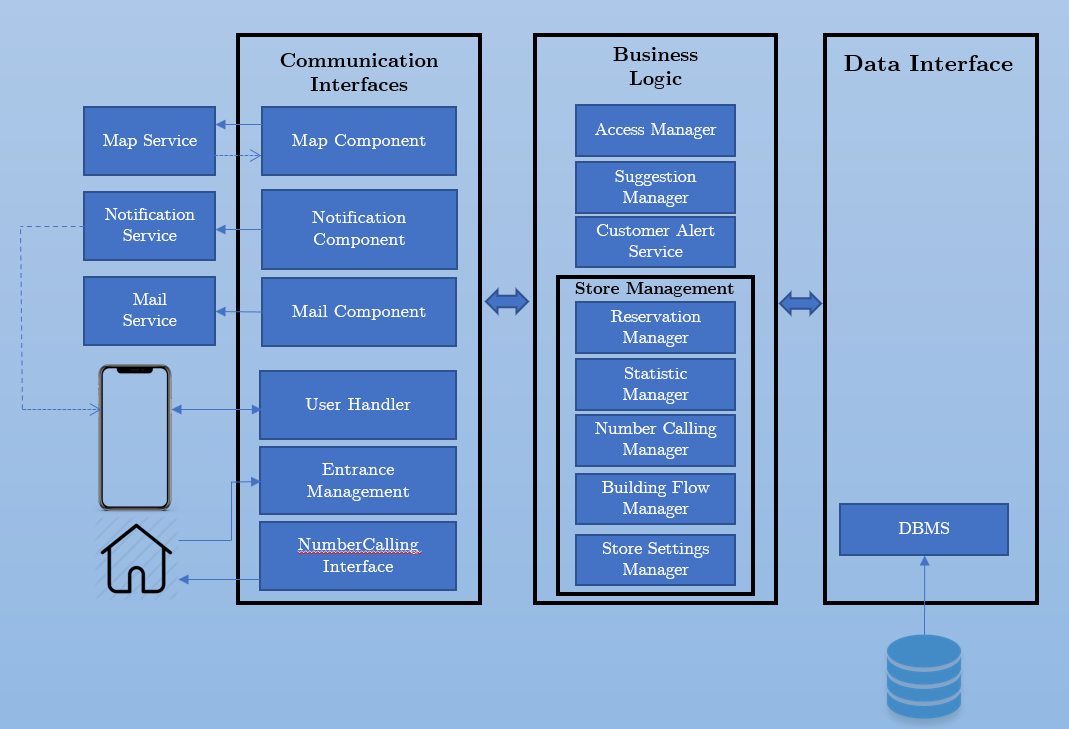
\includegraphics[scale=0.5]{../UML Diagrams/CompositionDiagram/CompositionDiagram.png} \\
		\end{adjustwidth}
		\caption{\emph{Number calling system}}
	\end{figure}
	
		\item{\bfseries Business Logic}: here there is the whole Business Logic of the system. Since each store may maintain a different logic from another, there is a Component for each store managed by the system. Each store, manages the following aspects:
		\begin{itemize}
			\item{\bfseries Reservation Manager}: manages all the things concerning reservations and their making. It's useful also to retrieve some important data, such as \emph{ETA}s and available time intervals to enter the store.
			\item{\bfseries Statistic Manager}: it's the part used for the calculation of statistics about customers' shopping time, and about the average time spent in a single department. Since each store is different from the other, the statistics are maintained unique per store. This part is also used by \textbf{Reservation Manager} to calculates \emph{ETA}s and time intervals;
			\item{\bfseries Number Calling System}: is the component dedicated to admit reserved customers inside the store.
			\item{\bfseries Building Flow Manager}: it takes care of processing scanned \emph{QR Codes} at the entry and the exit of the store.
			\item{\bfseries Store Settings Manager}: manages all the things concerning stores' settings and parameters, such as working hours and capacity (also for each department).
			
		\end{itemize} This subdivision allows to separate better the logic of each store. Moreover, there are component common to each store, so the ones designated to allow users to request services to the system.
		\begin{itemize}
			\item {\bfseries Access Manager}: manages users' registration and log-in;
			\item {\bfseries Suggestion Manager}: manages the retrieve of suggestions when required, or necessary;
			\item{\bfseries Customer Alert Service}: takes care of sending departing notifications to customers.
		\end{itemize}
	At the end, there is another block: the \textbf{Data Interface}: it represents the \emph{Data Tier} of the system and separates the Business Logic from the data. It interacts with the \emph{DBMS} to store and load informations.
	\end{itemize}

	
	\subsection{Component View}
		The aim of this section is to give a look to the architectural aspect of the analyzed system. In doing this, a top-down approach will be followed, starting from a very general view of the system, then going into more detail through {\bfseries Component Diagrams}, more and more detailed. This allows us to precisely describe each component of \emph{CLup}, so that who will develop the system would know the behaviour of each component.\\
		
		\begin{itemize}
			\item {\bfseries MobileApp}: it is the component relative to the mobile application used by store managers and customers; in order to access \emph{CLup} services. It uses three interfaces: \emph{CustomerInterface}, \emph{StoreInterface}, used to access functionalities respectively for customers and store managers, and \emph{AccessInterface}, that allows users to log-in and register. Moreover, uses \emph{MapsAPI} to access to cartographic services, and \emph{NotificationAPI} to send local notifications.
			
			\item {\bfseries CLupServer}:  it is the component designated to manage users’ access, and customers requests.
			
			\item {\bfseries StoreComponent}: it is the component that principally manages the business logic of the system, since takes care of the functionalities associated with a single store. Each store will have its own {\bfseries Store Component} deployed in a dedicated container. The aim of this is to separate the critical functionalities of each store, to reduce the risk of a complete block of the system and to make maintenance easier in case of dysfunctionality of a single store.
			
			\item {\bfseries TotemApp}: it is the component that represents the interface used by a physical totem installed at stores in order to request the issue of a ticket. The totem interface is separated from the Mobile App’s one, since a totem can request tickets only to the store where it’s installed, directly communicating with it.
			
			\item {\bfseries ScannerApp}: it is the component that represents \emph{QR Scanners}’, that asks the associated store to process the scanned \emph{QR Codes}.
			
			\item {\bfseries NumberCallingApp}: it is the component designated to notify at stores that a number has been called. It’s used by the associated store to notify that some customers are admitted to enter the store.		
		\end{itemize}
	
		Moreover, to exploit some features, \emph{CLup} relies on some external services, using them through their \emph{API}s:
		
		\begin{itemize}
			\item {\bfseries MapsAPI}: exploits the \emph{API}s of an external map services, necessary to compute percurrency times and sort stores depending on the position.
			
			\item {\bfseries NotificationAPI}: it is the interface used to send notifications to customers’ devices. Since each mobile \emph{OS} already has its own notification system, \emph{CLup} exploits this in sending notifications, without the need of building a new in-house notification service.
			
			\item {\bfseries EmailAPI}: it is the interface used to communicate with a mail provider service, to send emails to customers.
			
			\item {\bfseries DBMSAPI}: the interface used to access the Data Logic of \emph{CLup}.
		\end{itemize}
	
		It has been chosen to not develop these features, since there isn’t a real necessity of making them from scratch: the existing ones work well, are already tested and complete (for example, developing an internal map service will require inserting the whole world cartography, while a non \emph{OS}-integrated notification service must deal with aggressive \emph{OS}es’ power management). Moreover, this outsourcing allows to reduce the time for developing the system, and the maintenance costs, since it’s externally done by the service provider.
		
		

		\begin{figure}
			\begin{adjustwidth} {-3cm}{}
				\centering
				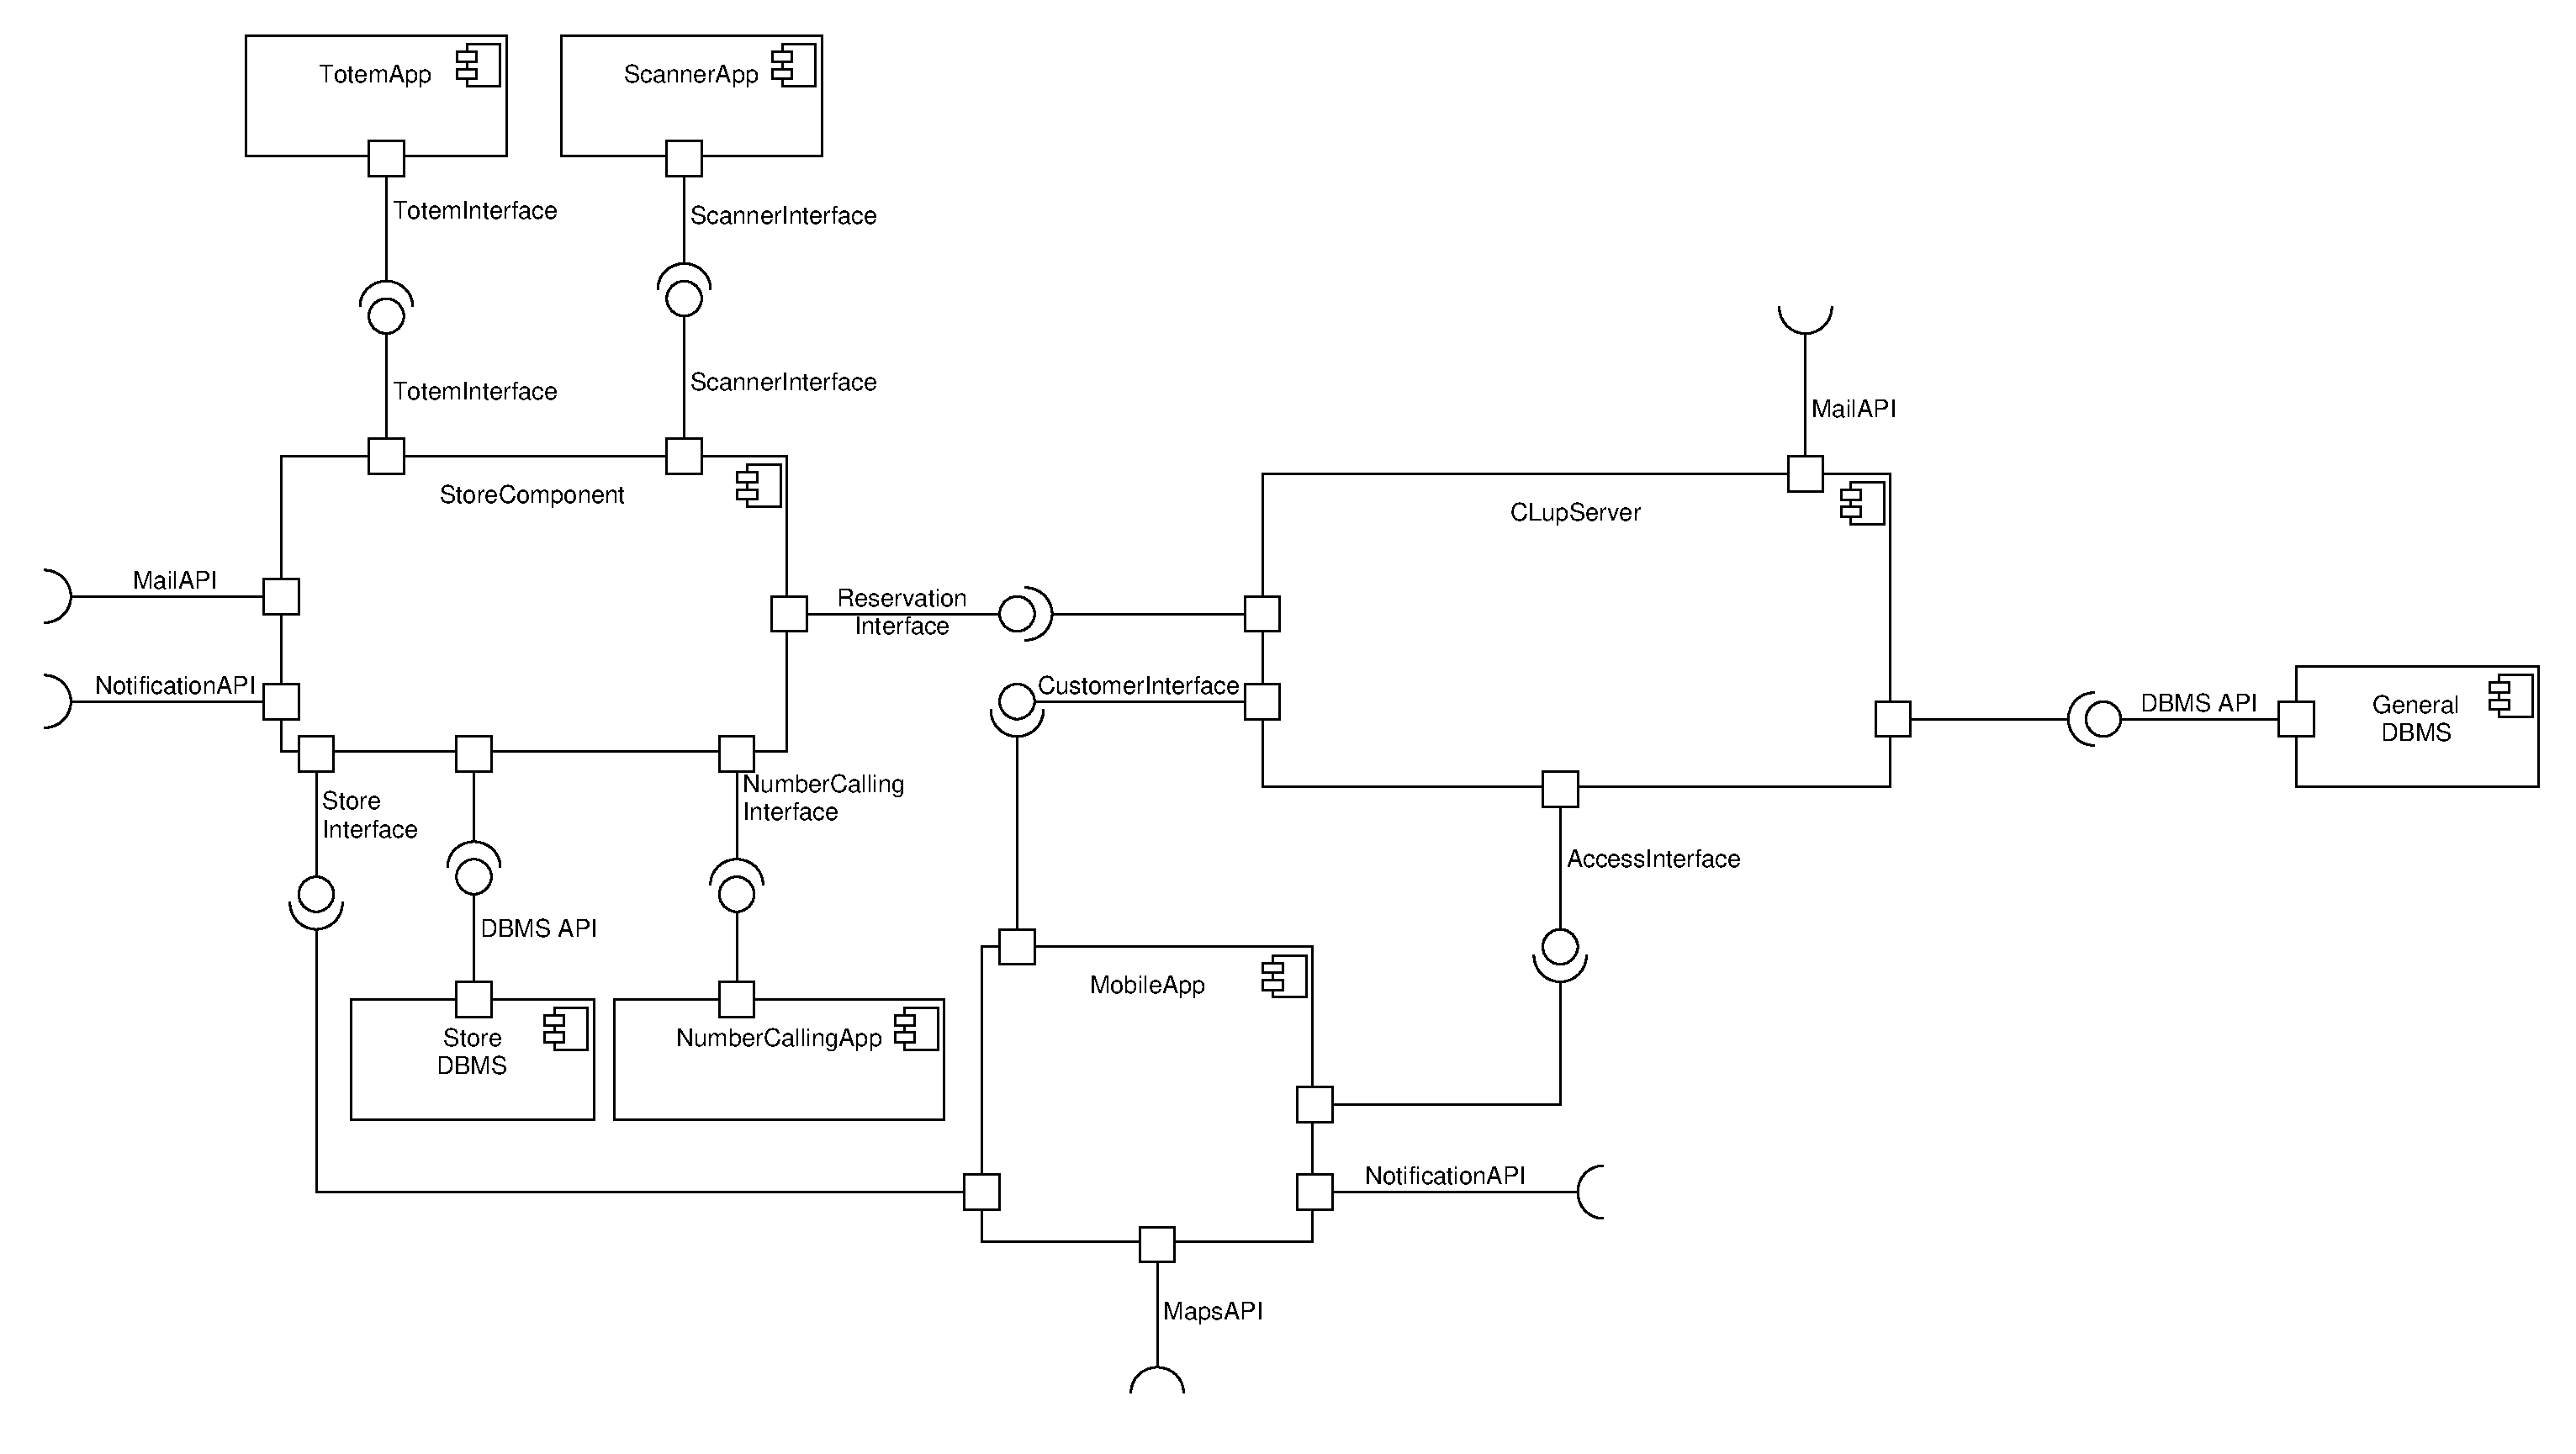
\includegraphics[scale=0.35, angle=90, trim= 0 0 0 -5cm]{Component Diagrams/HighLevelComponentDiagram.pdf}\\
			\end{adjustwidth}
			\caption{\emph{High Level Component Diagram}}
		\end{figure}
		\newpage
		
		\subsubsection{Adapters}
		The system uses some “Adapters” to access the external services; no \emph{API}s are directly exposed to any component but the adapters. So, it is sufficient to change the corresponding adapter to migrate to another service, without the need of rewriting code of other components. Moreover, if required in some circumstances, it’s possible to use different external services: it is sufficient to use the correct adapter in order to access the desired service.
		
		\begin{itemize}
			\item {\bfseries MapManager}: it is the component that takes requests from other components, and redirects them to the chosen external {\bfseries Map Service}.
			
			\item {\bfseries NotificationComponent}: since each mobile \emph{OS} uses its own notification service, this adapter takes in requests of notification sending, and redirects them to the correct service; the latter will take care of delivering the notification to the customer.
			
			\item {\bfseries MailComponent}: an adapter used to send emails; as the previous ones, allows to change the used mail service painlessly.
			
			\item {\bfseries DataManager}: probably, the most important adapter of the system, since it is the one connecting the other components to the system’s data logic. 
		\end{itemize}
		
		
		Here, there is described the adapter for \emph{DBMS}, since it’s the most articulated among those.
		
			\paragraph{Data Manager Component}
				The Data Manager is the component that manages the requests for data manipulation. The component handles two aspects:
				
				\begin{itemize}
					\item Data Manipulation
					\item Query Execution
				\end{itemize}
			
				The components’ services are requested through the \emph{DataInterface}, while it access to the \emph{DBMS} through its \emph{API}s. Data can be accessed or written to the \emph{DBMS}. This partition is very important because it allows to separate the query for obtaining data from the ones to manipulate the databse.
				
				\begin{itemize}
					\item {\bfseries DataRequestor}: it is the component that manages the data reading. Indeed if \emph{DataInterface} asks for a data, this component allows to satisfy this request.
					
					\item {\bfseries DataStorer}: it is the component that manages the data writing. Indeed if \emph{DataInterface} asks to manipulate the \emph{DBMS}, this component allows to satisfy this request.
					
					\item {\bfseries QueryExecutor}: it is the component that manages the connection with the \emph{DBMS}. It uses the \emph{DBMSAPI} and both \emph{DataRequestor} and \emph{DataStorer} rely on him to interface directly with the database.
					
				\end{itemize}
			
				\begin{figure}
					\begin{adjustwidth} {-1cm}{}
						\centering
						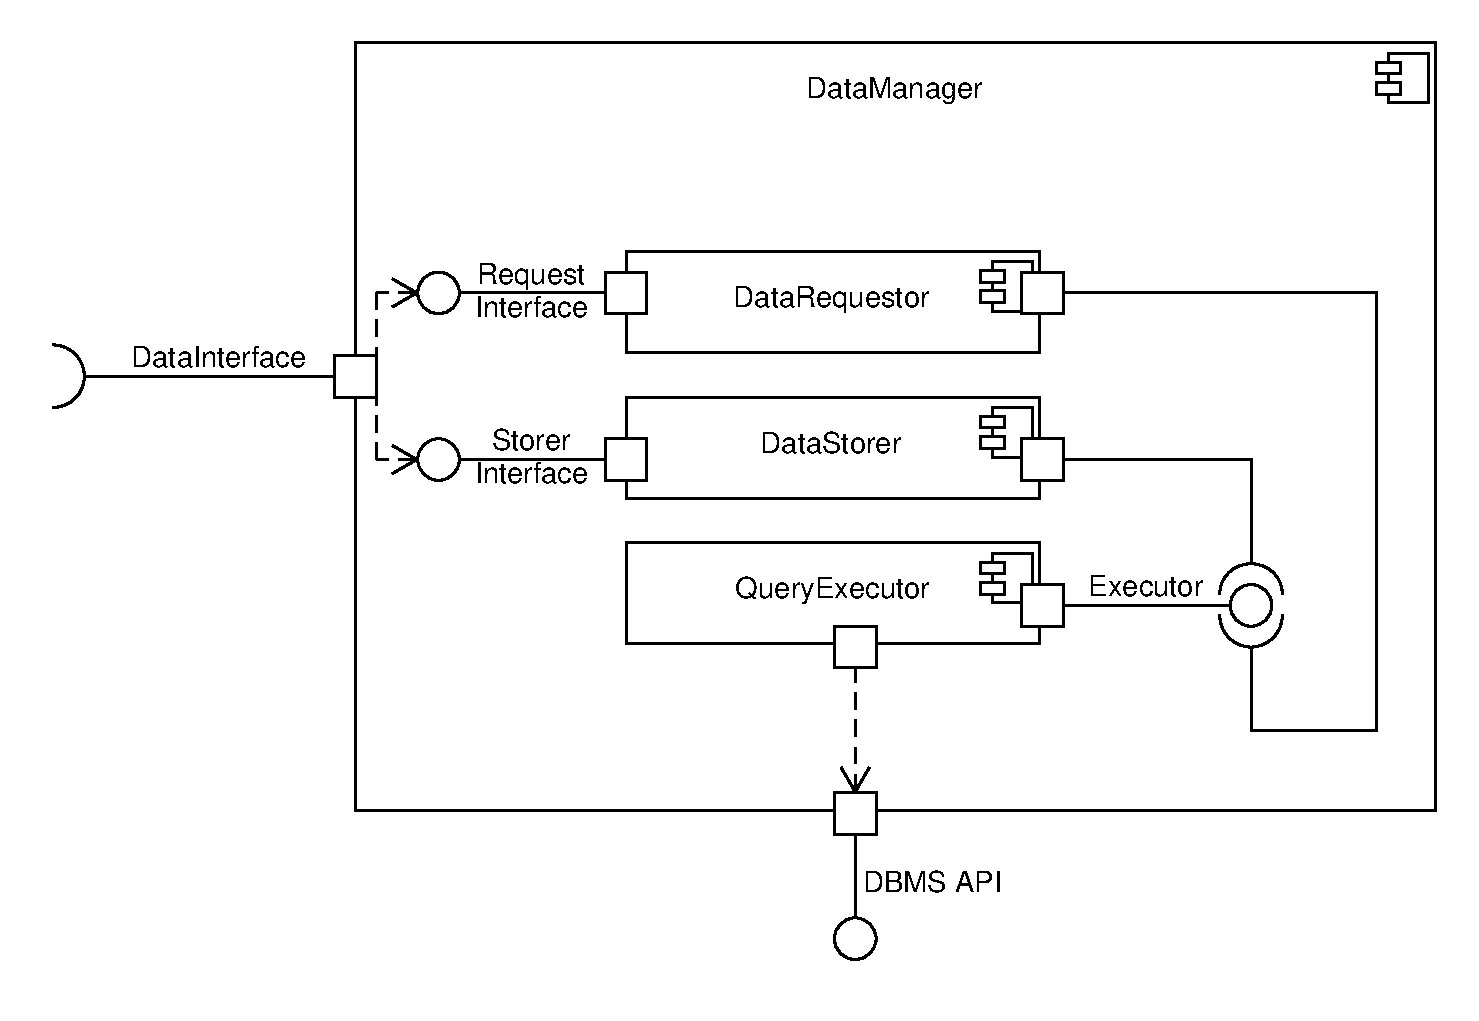
\includegraphics[scale=0.5]{Component Diagrams/DataManagerComponentView.pdf}\\
					\end{adjustwidth}
					\caption{\emph{Data Manager Component View}}
				\end{figure}
			
			\subsubsection{CLup Server}
			As said before, it manages customers’ requests and access operations, through the two interfaces it expose:
			
			\begin{itemize}
				\item {\bfseries CustomerInterface}: expose all the methods relative to services a customer can access, such as making a reservation and retrieving already made reservations.
				
				\item {\bfseries AccessManager}: the interface designated to manage login and registration of users. After a login, will send to the user the correct set of operations the user can do, depending on their role: customers or store managers.
			\end{itemize}
			
			In the following paragraphs, there is a description of the most relevant component contained in {\bfseries \emph{CLup} Server}.
			\begin{figure}
				\begin{adjustwidth} {0cm}{}
					\centering
					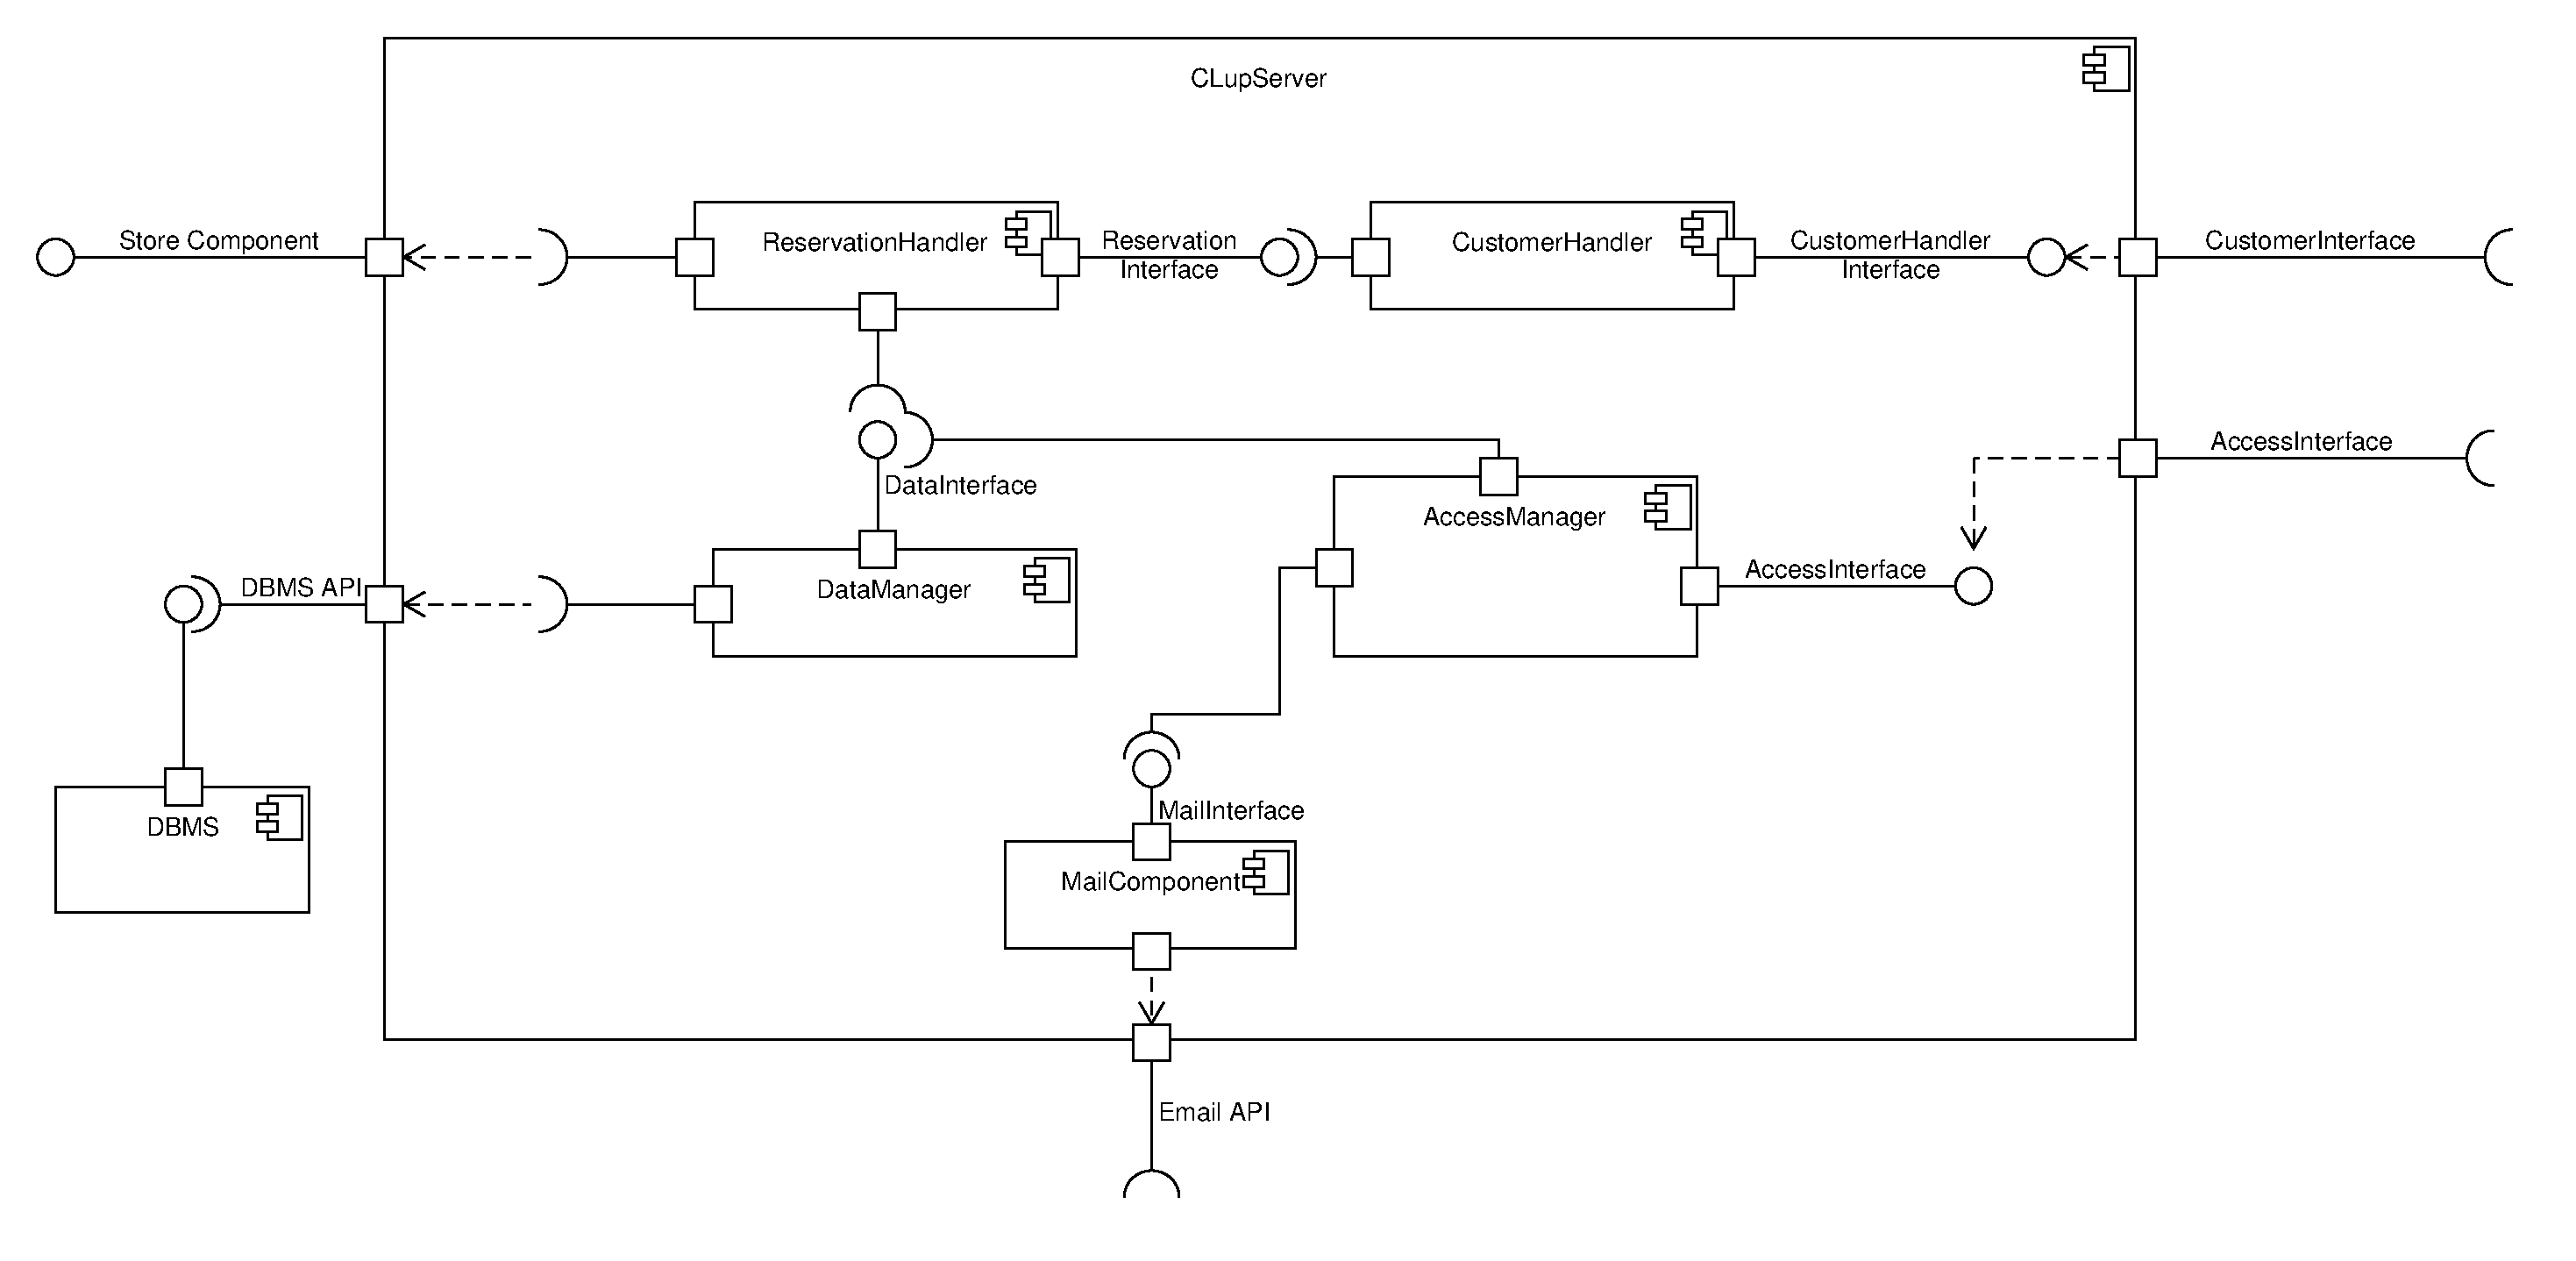
\includegraphics[scale=0.37, angle=90, trim= 0 0 0 -5cm]{Component Diagrams/ServerComponentView.pdf}\\
				\end{adjustwidth}
				\caption{\emph{Server Component View}}
			\end{figure}
			\newpage
				\paragraph{Customer Handler Component}
					The CustomerHandler is the component that manages all the actions that a customer can make within the application. The component analyzes the aspects concerning reservations.
					
					This component is used by invoking methods on the \emph{CustomerHandlerInterface}. This component is divided in some subcomponents:
					
					\begin{itemize}
						\item {\bfseries ASAPManager}: it is the component that manages the \emph{ASAP} reservations and it is formed from two sub-component: {\bfseries DeleteRes} and {\bfseries AddRes}. The first one deals with deleting an \emph{ASAP} reservation while the second one deals with creating a new \emph{ASAP} reservation.
						
						\item {\bfseries BookingManager}: it is the component that manages the booking via app and it is formed from three sub-component: {\bfseries DeleteRes}, {\bfseries ModifyRes} and {\bfseries AddRes}. The first one deals with deleting a reservation, the second one deals with modifying a reservation while the third one deals with adding new reservations. 
						
						\item {\bfseries RetrieveReservation}: it is the component that is used to retrieve and update all user’s reservations.
					\end{itemize}
				
					All of these components uses the \emph{ReservationInterface} to complete their tasks.
					\bigskip
					\begin{figure}[h]
						\begin{adjustwidth} {-4cm}{}
							\centering
							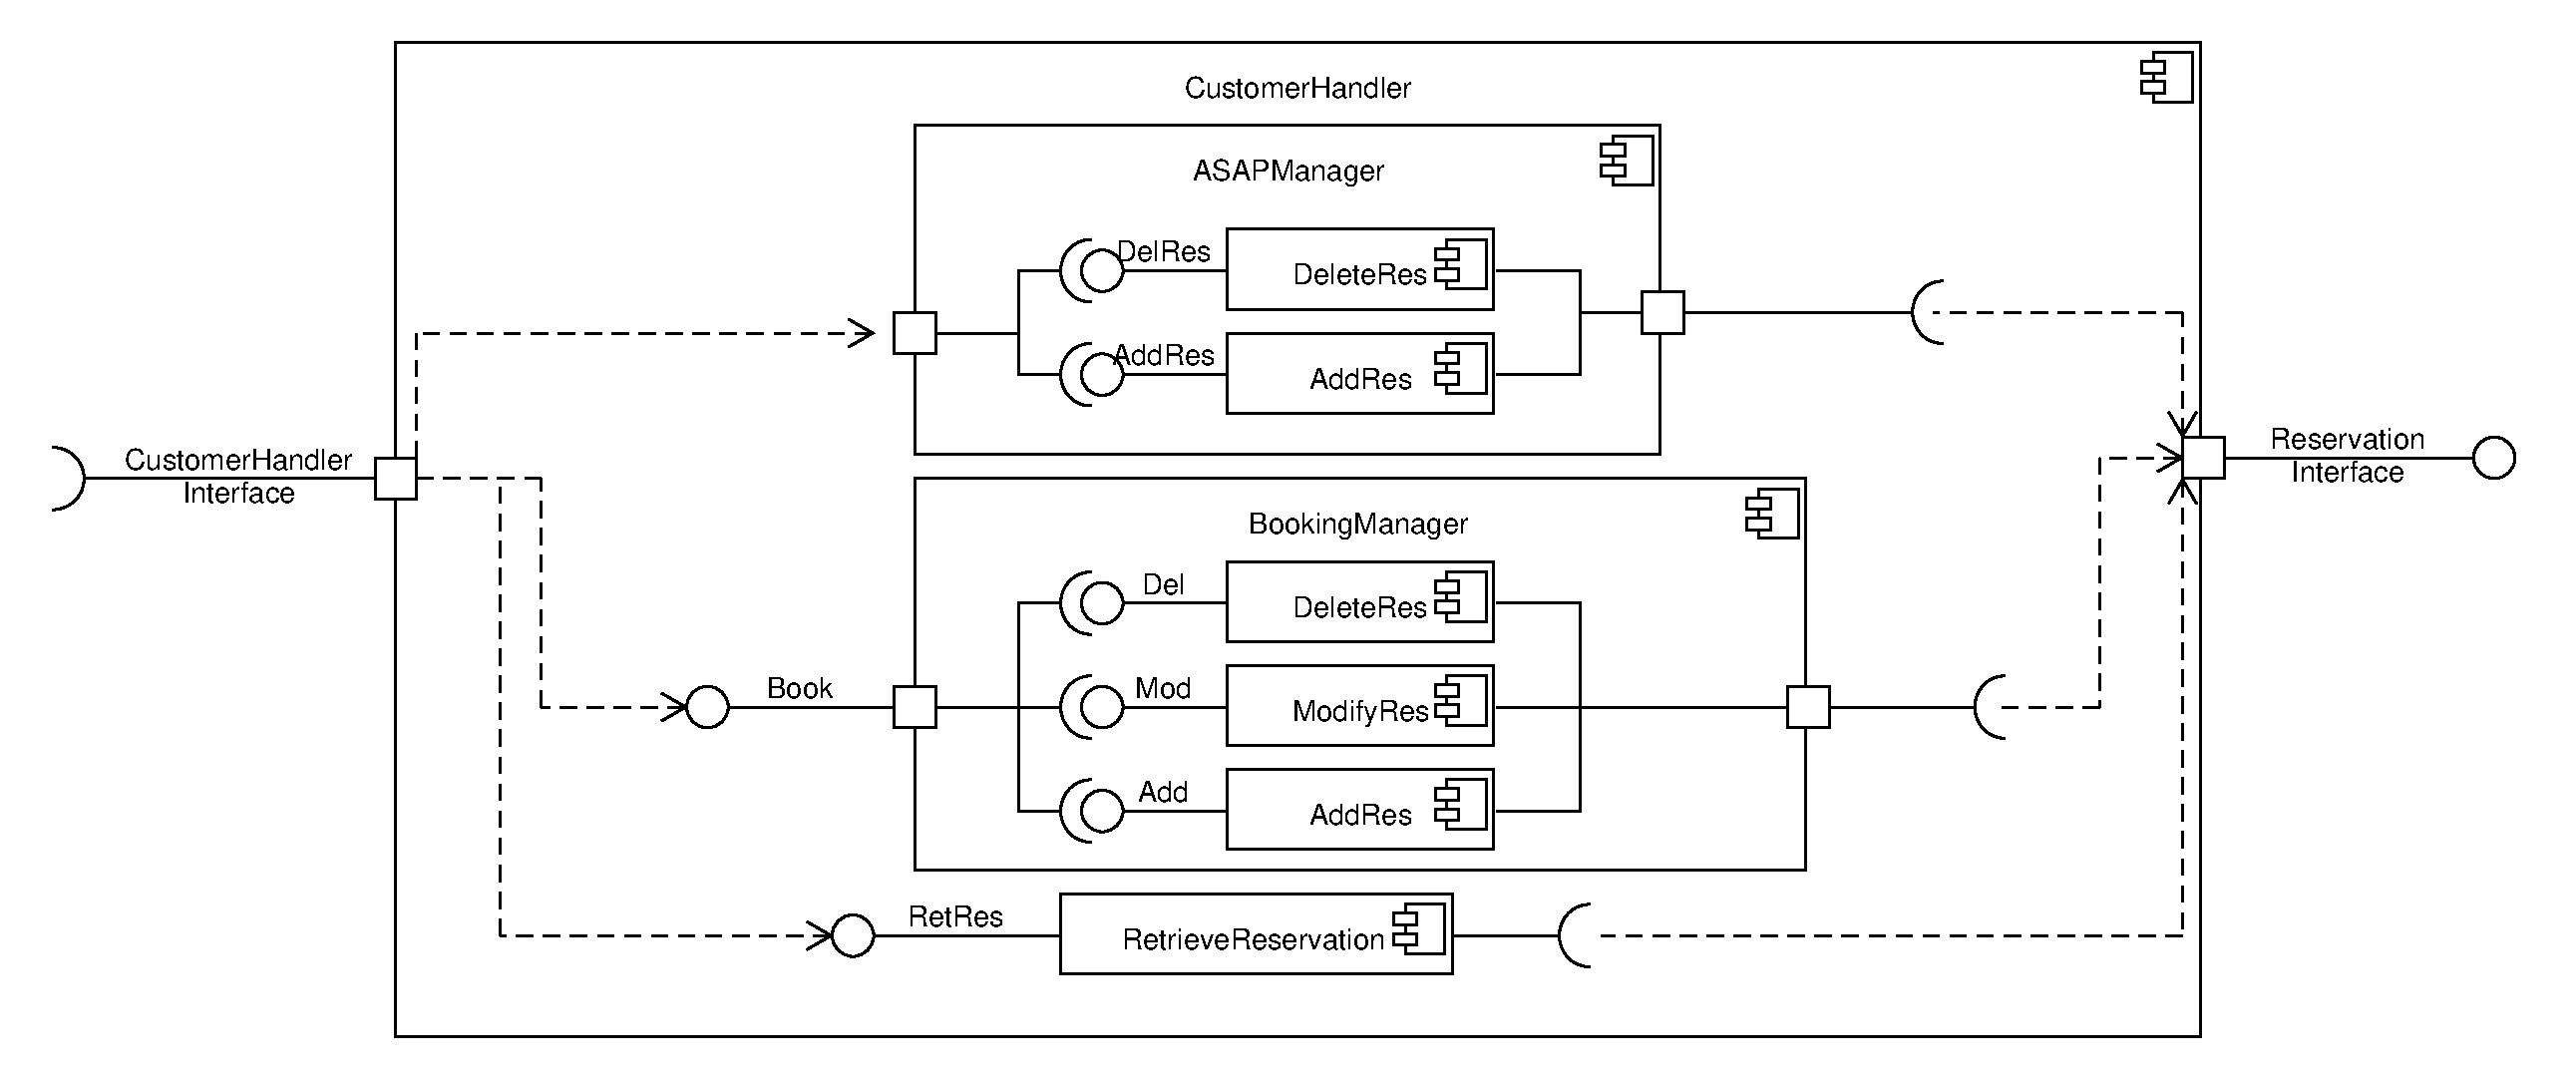
\includegraphics[scale=0.45]{Component Diagrams/CustomerHandlerComponentView.pdf}\\
						\end{adjustwidth}
						\caption{\emph{Customer Handler Component View}}
					\end{figure}
				\newpage
				\paragraph{Access Manager Component}
					The Access Manager is the component that manages all the issues concerning the access of the users. Indeed, as mentioned above, it is very important to recognize the role of the users in the app in order to provide them correct information, and only the functionalities/data they are authorized to use. The component analyzes two main aspects:
					
					\begin{itemize}
						\item Login
						\item Registration
					\end{itemize}
				
					The component uses two very important interfaces: \emph{EmailAPI} and \emph{DataInterface}. The first one is used for the registration, in order to send confirmation messages, while the second one is used for storing registration data, and to check credentials for log-in operations. Furthermore, its services are requested through the \emph{AccessInterface}, that implements the interfaces exposed by {\bfseries Login Component}, and {\bfseries Registration Component}. This component is invoked by \emph{StoreManagerAccessInterface} and \emph{CustomerAccessInterface} in case an user wants to log in or register
					
					\begin{itemize}
						\item {\bfseries LoginManager}: it is the component that manages user’s login. Indeed, if a user logs in, the component checks if the credentials are correct and then allows the user to use their personal area.
						
						\item {\bfseries RegistrationManager}: it is the component that manages the user’s registration. Indeed, if a user makes a registration, this component, at the beginning, checks through \emph{DataInterface} if the data inserted by the user are valid (e.g. uniqueness of the email, or certification for store managers). Then, if the data are correct, the user’s data are stored in the \emph{DBMS}.
						
						\begin{itemize}
							\item {\bfseries RegistrationChecker}: it is the component that checks if the information is inserted during the registration, from the user, are valid. In case of customers, this component checks if the email is valid while in case of store manager checks if the store certification is valid and the registration \emph{ID} is unique.
							
							\item {\bfseries RegistrationStorer}: it is the component that stores the new data in the \emph{DBMS} after checking.
						\end{itemize}
					\end{itemize}
				
				\begin{figure}[h]
					\begin{adjustwidth} {-2.5cm}{}
						\centering
						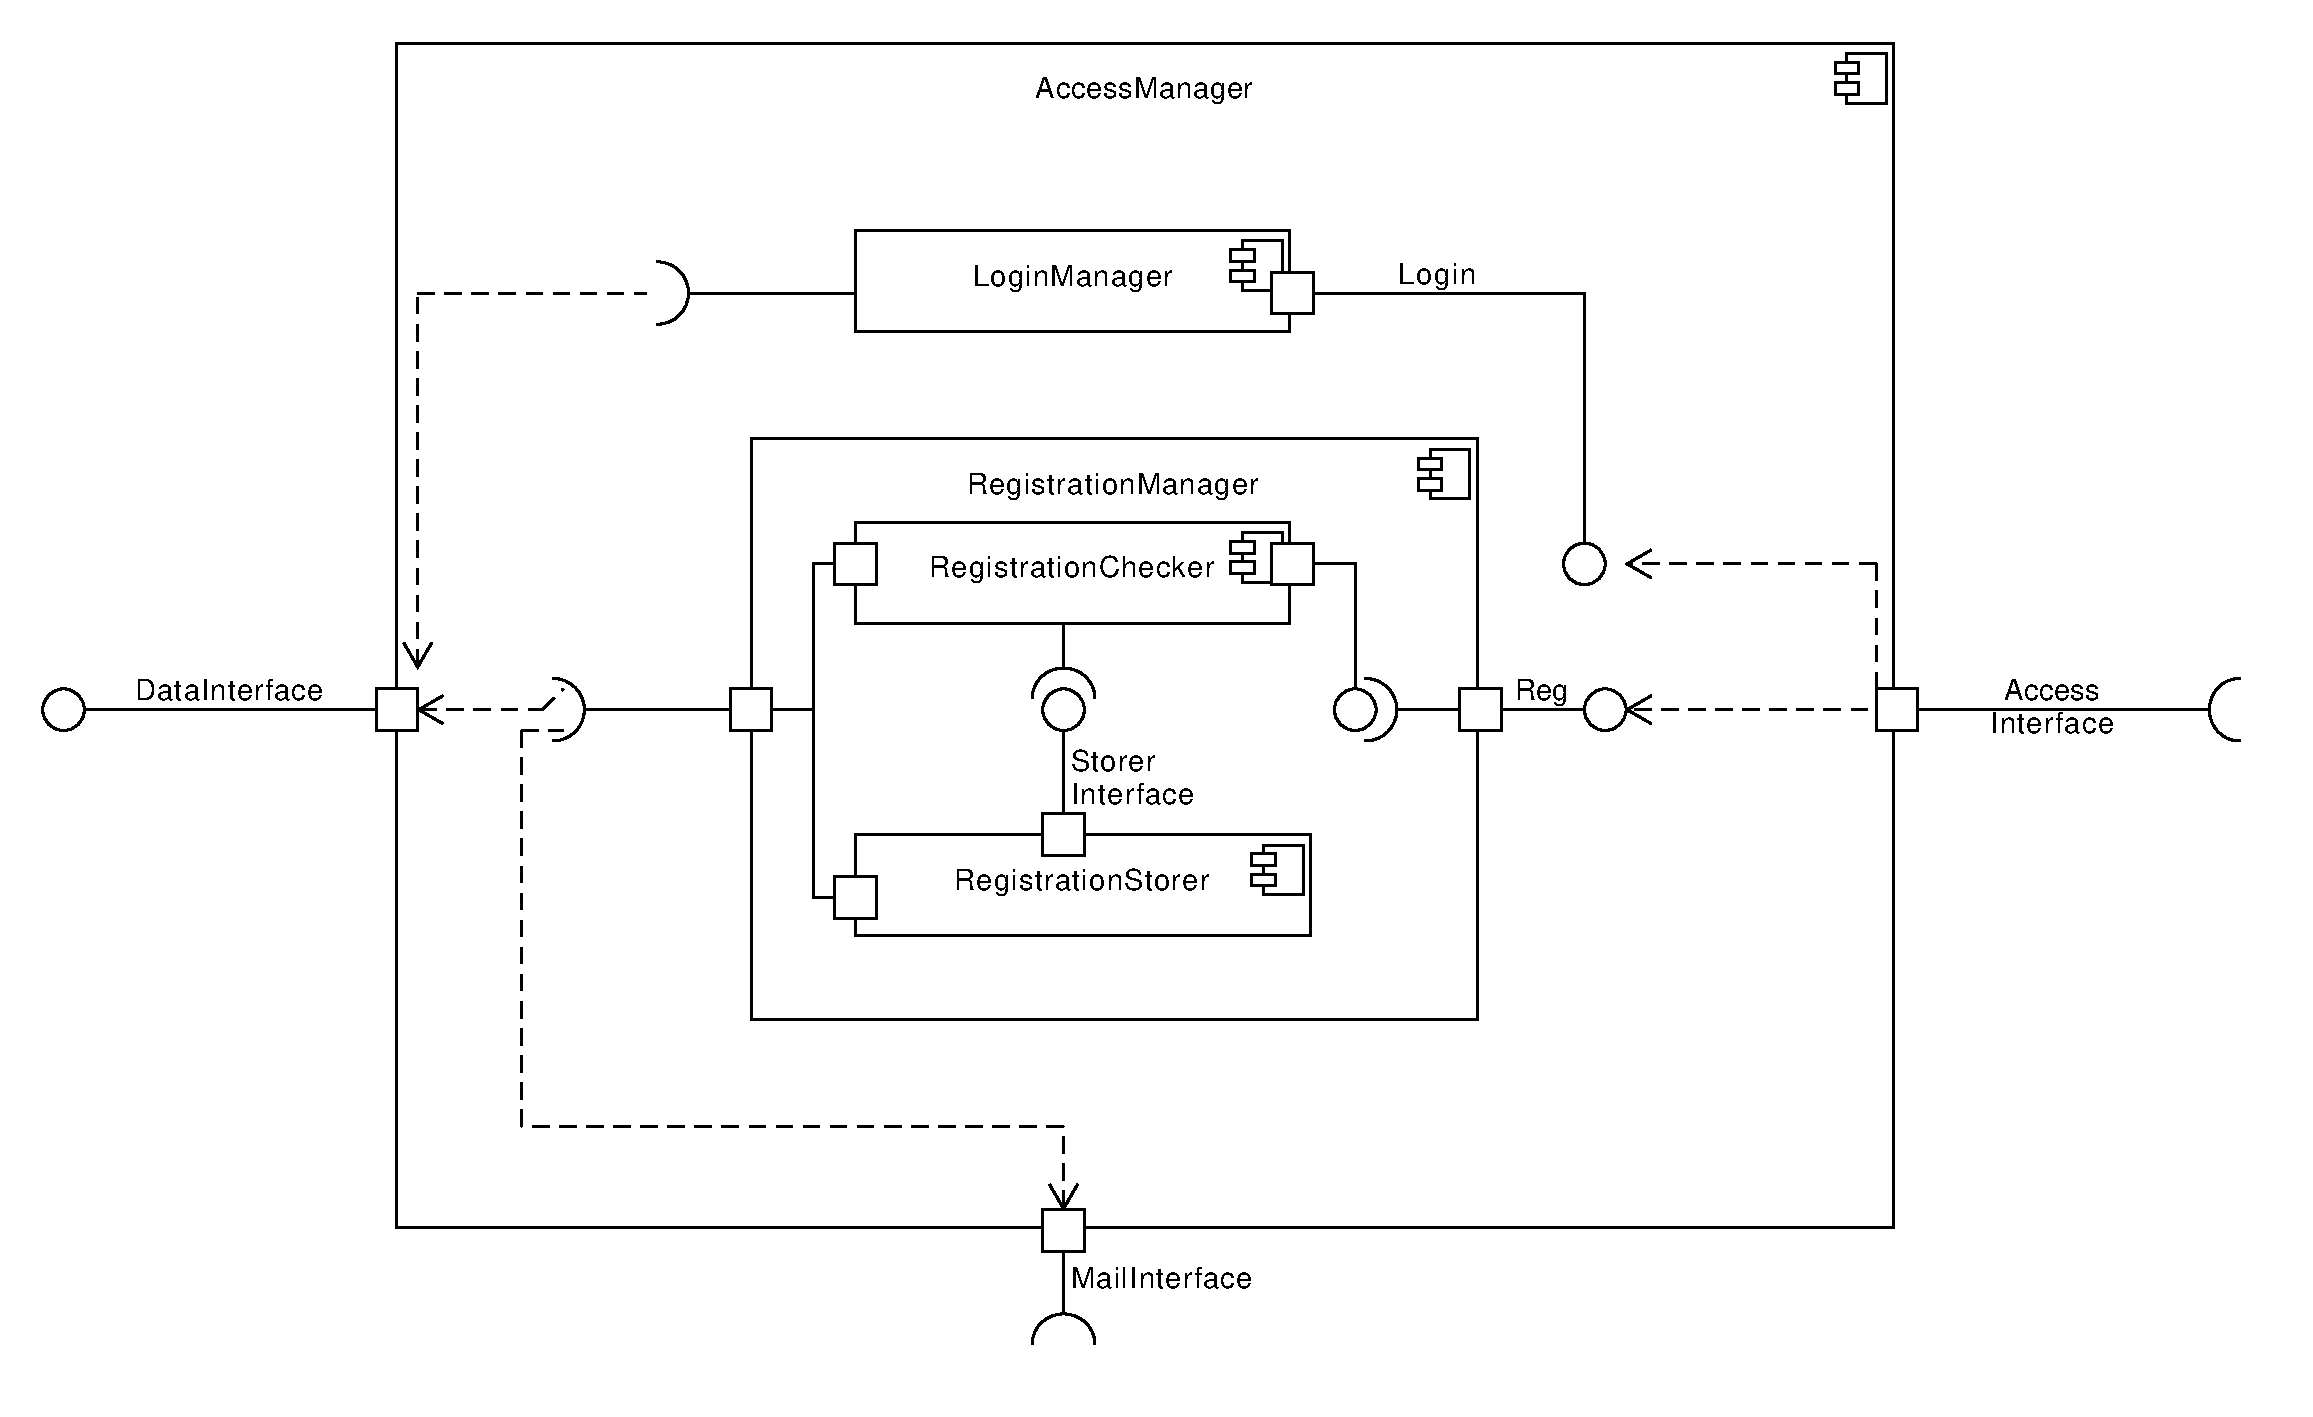
\includegraphics[scale=0.45]{Component Diagrams/AccessManagerComponentView.pdf}\\
					\end{adjustwidth}
					\caption{\emph{Access Manager Component View}}
				\end{figure}
				\newpage
				
			\paragraph{Reservation Handler Component}
				The Reservation Handler is the component that manages the customer’s reservations. The component analyzes two main aspects:
				
				\begin{itemize}
					\item Suggestions
					\item Reservation Management
				\end{itemize}
			
				The component uses \emph{ReservationInterface} (that implements \emph{QueryInterface} and \emph{SuggestionInterface}) to accept requests, and {\bfseries Store Component}, used to make requests to a specific store.
				This component is invoked when the customer tries to make or modify a reservation, or tries to retrieve his ones. Each time a reservation is retrieved, the customer will receive the updated information (such us \emph{ETA} to enter the store). Moreover, it uses the \emph{Data Interface} to access to \emph{CLup}'s general \emph{DBMS}, in order to retrieve informations on stores.
				
				\begin{itemize}
					\item {\bfseries SuggestionComponent}: it is the component that manages the suggestions that are made available to the customer at the time of reservation. It will query each store registered on the platform, to retrieve availability information, depending on the preferences inserted by the customer and the type of reservation they are making (so, the component will use the right {\bfseries Query Component}); it’s invoked by both the \emph{ReservationInterface} when a customer asks for suggestions on bookings, or by {\bfseries ASAPQueryComponent} while the \emph{ETA} for entering the store \emph{ASAP} is too high.
					
					\item {\bfseries StoreQueryComponent}: it is the component that manages the queries that are made at a particular store, indeed this component uses the {\bfseries Store Component}. The queries can be of two types:
					
					\begin{itemize}
						\item {\bfseries ASAPQueryComponent}: it is the component that manages the \emph{ASAP} reservation, asks the server for waiting times for accessing the store, notifies the store if a reservation is made and manages the deletion of \emph{ASAP} reservations.
						
						\item {\bfseries BookingQueryComponent}: it is the component that manages the booking via app, asking the server time slots to enter the store, in case a reservation is confirmed, notify the store to save it, and manages all the requests about modification and cancellation of booking reservations.		
					\end{itemize}
				\end{itemize}
				\bigskip
				\begin{figure}[h]
					\begin{adjustwidth} {-0.5cm}{}
						\centering
						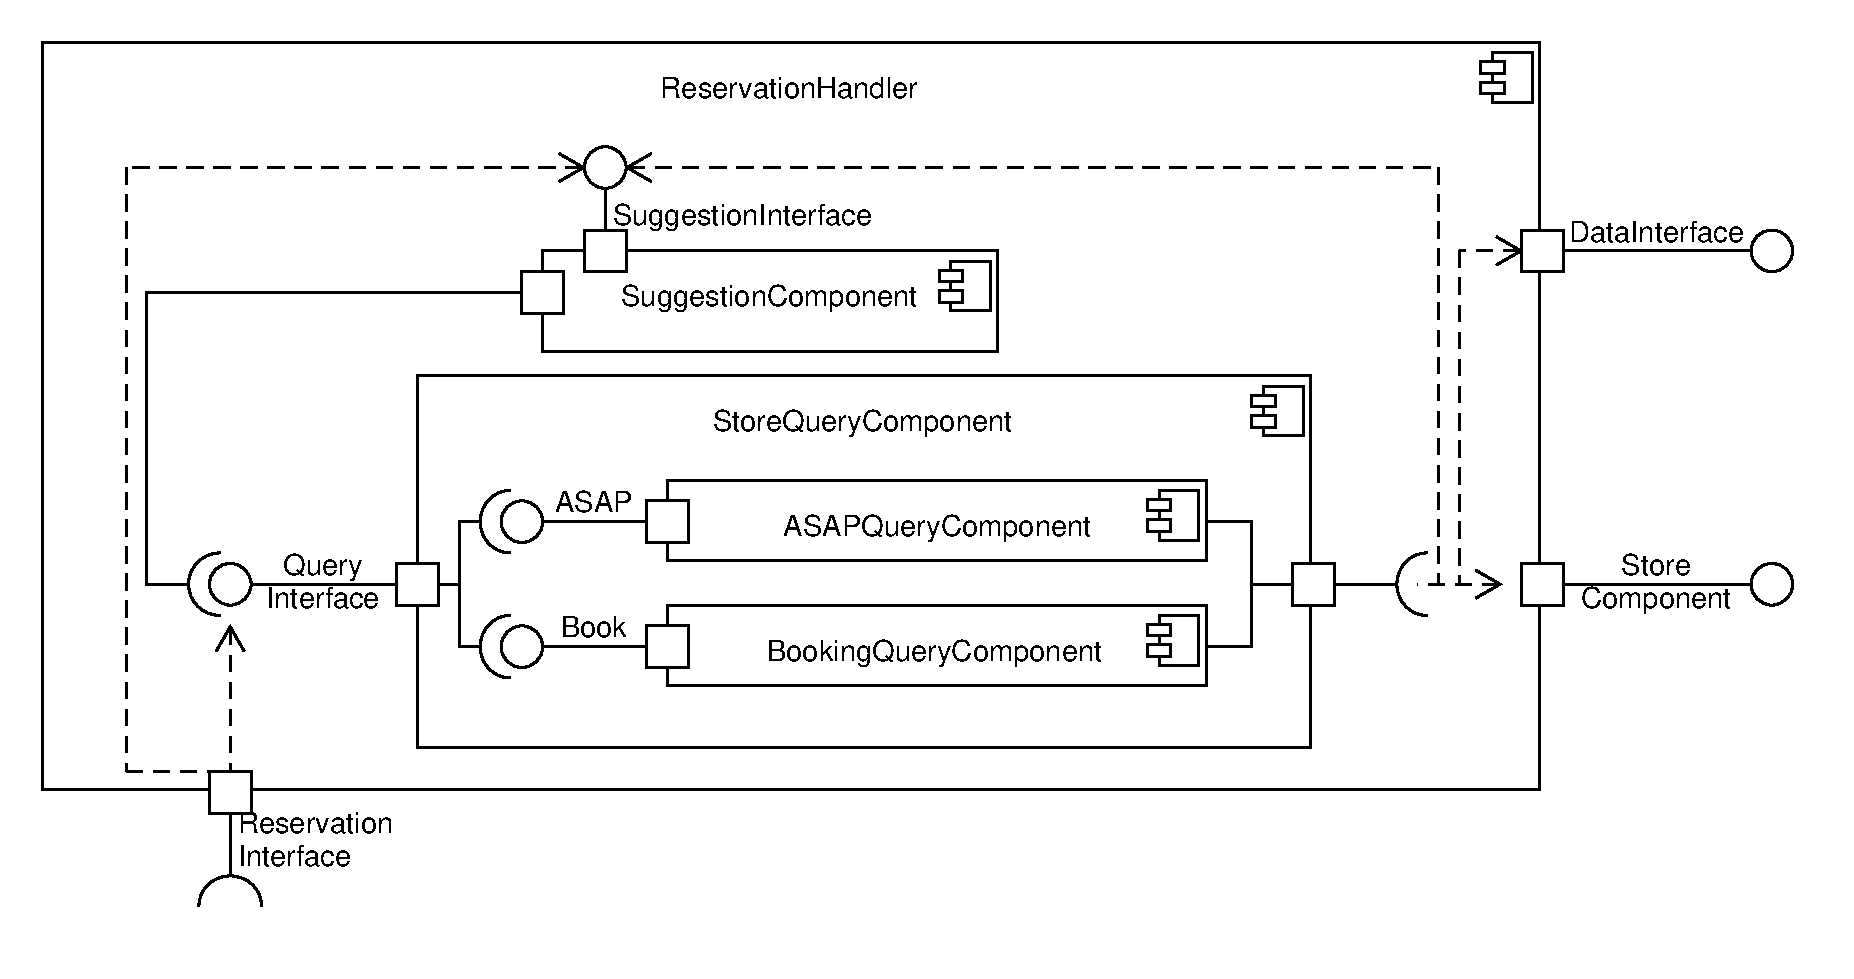
\includegraphics[scale=0.5]{Component Diagrams/ReservationHandlerComponentView.pdf}\\
					\end{adjustwidth}
					\caption{\emph{Reservation Handler Component View}}
				\end{figure}
				\newpage
			
		\subsubsection{Store Component}
			The Store is the component that manages the store from all points of view and it is the most important component of the whole architecture, since implements the whole business tier. The component analyzes many important aspects, but the most important are:
			
			\begin{itemize}
				\item Reservation
				\item Admit Reservations Inside
				\item Store Parameters
				\item Statistical Values
			\end{itemize}
		
			As said before, it’s been preferred to separate the logic governing each store by designing a component for each different store. Also here, the store component have been designed in a modular way, to separate the different features offered by a single store; these are:
			
			\begin{itemize}
				\item {\bfseries FlowComponent}: this component manages the functionalities that are requested when a \emph{QR Code} is scanned at the store entry, and uses the {\bfseries Calling Number Component} to check the scanned \emph{QR Code} status, the {\bfseries Department Component} to register the entrance/exit and the {\bfseries StatisticComponent} to update visit statistics.
				
				\item {\bfseries StatisticComponent}: it is the component dedicated to building customer statistics. It’s used by:
				
				\begin{itemize}
					\item {\bfseries EntranceComponent}: in order to update visiting statistics at customers’ exit
					\item {\bfseries ReservationComponent}: invokes the methods when, during a reservation process, it’s necessary to infer the estimation of customers’ shopping time.
				\end{itemize}
			
				\item {\bfseries RearrangeComponent}: it is the component that rearrange the reservations when a store manager modifies the capacity of some part of the store, or some reservations are changed, and the queue must be reschedules. Interacts with the {\bfseries Calling Number Component} in order to rearrange the queue. In case of delays or cancellations, the customers will receive a notification.
				
				\item {\bfseries StoreDataManager}: it is the adapter between the store and its dedicated \emph{DBMS}. The choice of dedicating a \emph{DBMS} for each store is due to efficiency and security reasons: if a \emph{DBMS} breaks, it wouldn't affect the whole system, while a store can access only its data.
				
				\item {\bfseries ParameterManager}: it is the component that manages the parameters of the store, the settings and the situation of each department of the store. It’s used by:
				
				\begin{itemize}
					\item {\bfseries FlowComponent}: is used to update Departments’ situation.
					\item {\bfseries StoreManagerHandler}: is used to update store parameters, and to access the real-time situation of the store.
					\item {\bfseries ReservationComponent}: is used to request store situation in order to make a reservation.
				\end{itemize}
			
				Moreover, uses {\bfseries RearrangeReservation} when a parameter is modified, to make coherent the store’s status
				
				\item {\bfseries ReservationComponent}: it is the component that is dedicated to the management of reservations. It’s used to retrieve reservations made in that store, to retrieve waiting times, and to store customers’ reservations. Uses the {\bfseries Calling Number Component} to notify a modification in reservations list, and it’s used by the latter to initialize the queue at store opening. It also handles modifications made by customers and store managers to reservations. Furthermore, a store manager uses it to contact customers about some specific reservation. Because of this, the components interact with {\bfseries Notification Component} and {\bfseries Mail Component} to interact with customers. 
				To logically separate the management of the two types of reservations, the component is divided in two subcomponents: {\bfseries BookingComponent}, and {\bfseries ASAPComponent}.
				
				\item {\bfseries CallingNumberComponent}: it is the component designated to call in reservations, and to notify customers they should depart for the store. It’s divided in two subcomponents, each carrying out different functionalities:
				
				\begin{itemize}
					\item {\bfseries CallableReservationComponent}: checks whenever a reservation in the queue is callable, checking the store affluence, through the {\bfseries Parameter Manager Component};
					
					\item {\bfseries CallNumberComponent}: takes a queue of reservations to be called, and when it’s possible, a reservation is called to enter. It’s alerted by the {\bfseries Entrance Component} that somebody exited the store.
				\end{itemize}
			\end{itemize}
		
			The core store functionalities are requested through the \emph{ReservationInterface} (dedicated to customers’ features) and the \emph{StoreInterfaces}, dedicated to store managers; their requests pass through an handler, here described. 
			
			\begin{figure}[H]
				\begin{adjustwidth} {-1cm}{}
					\centering
					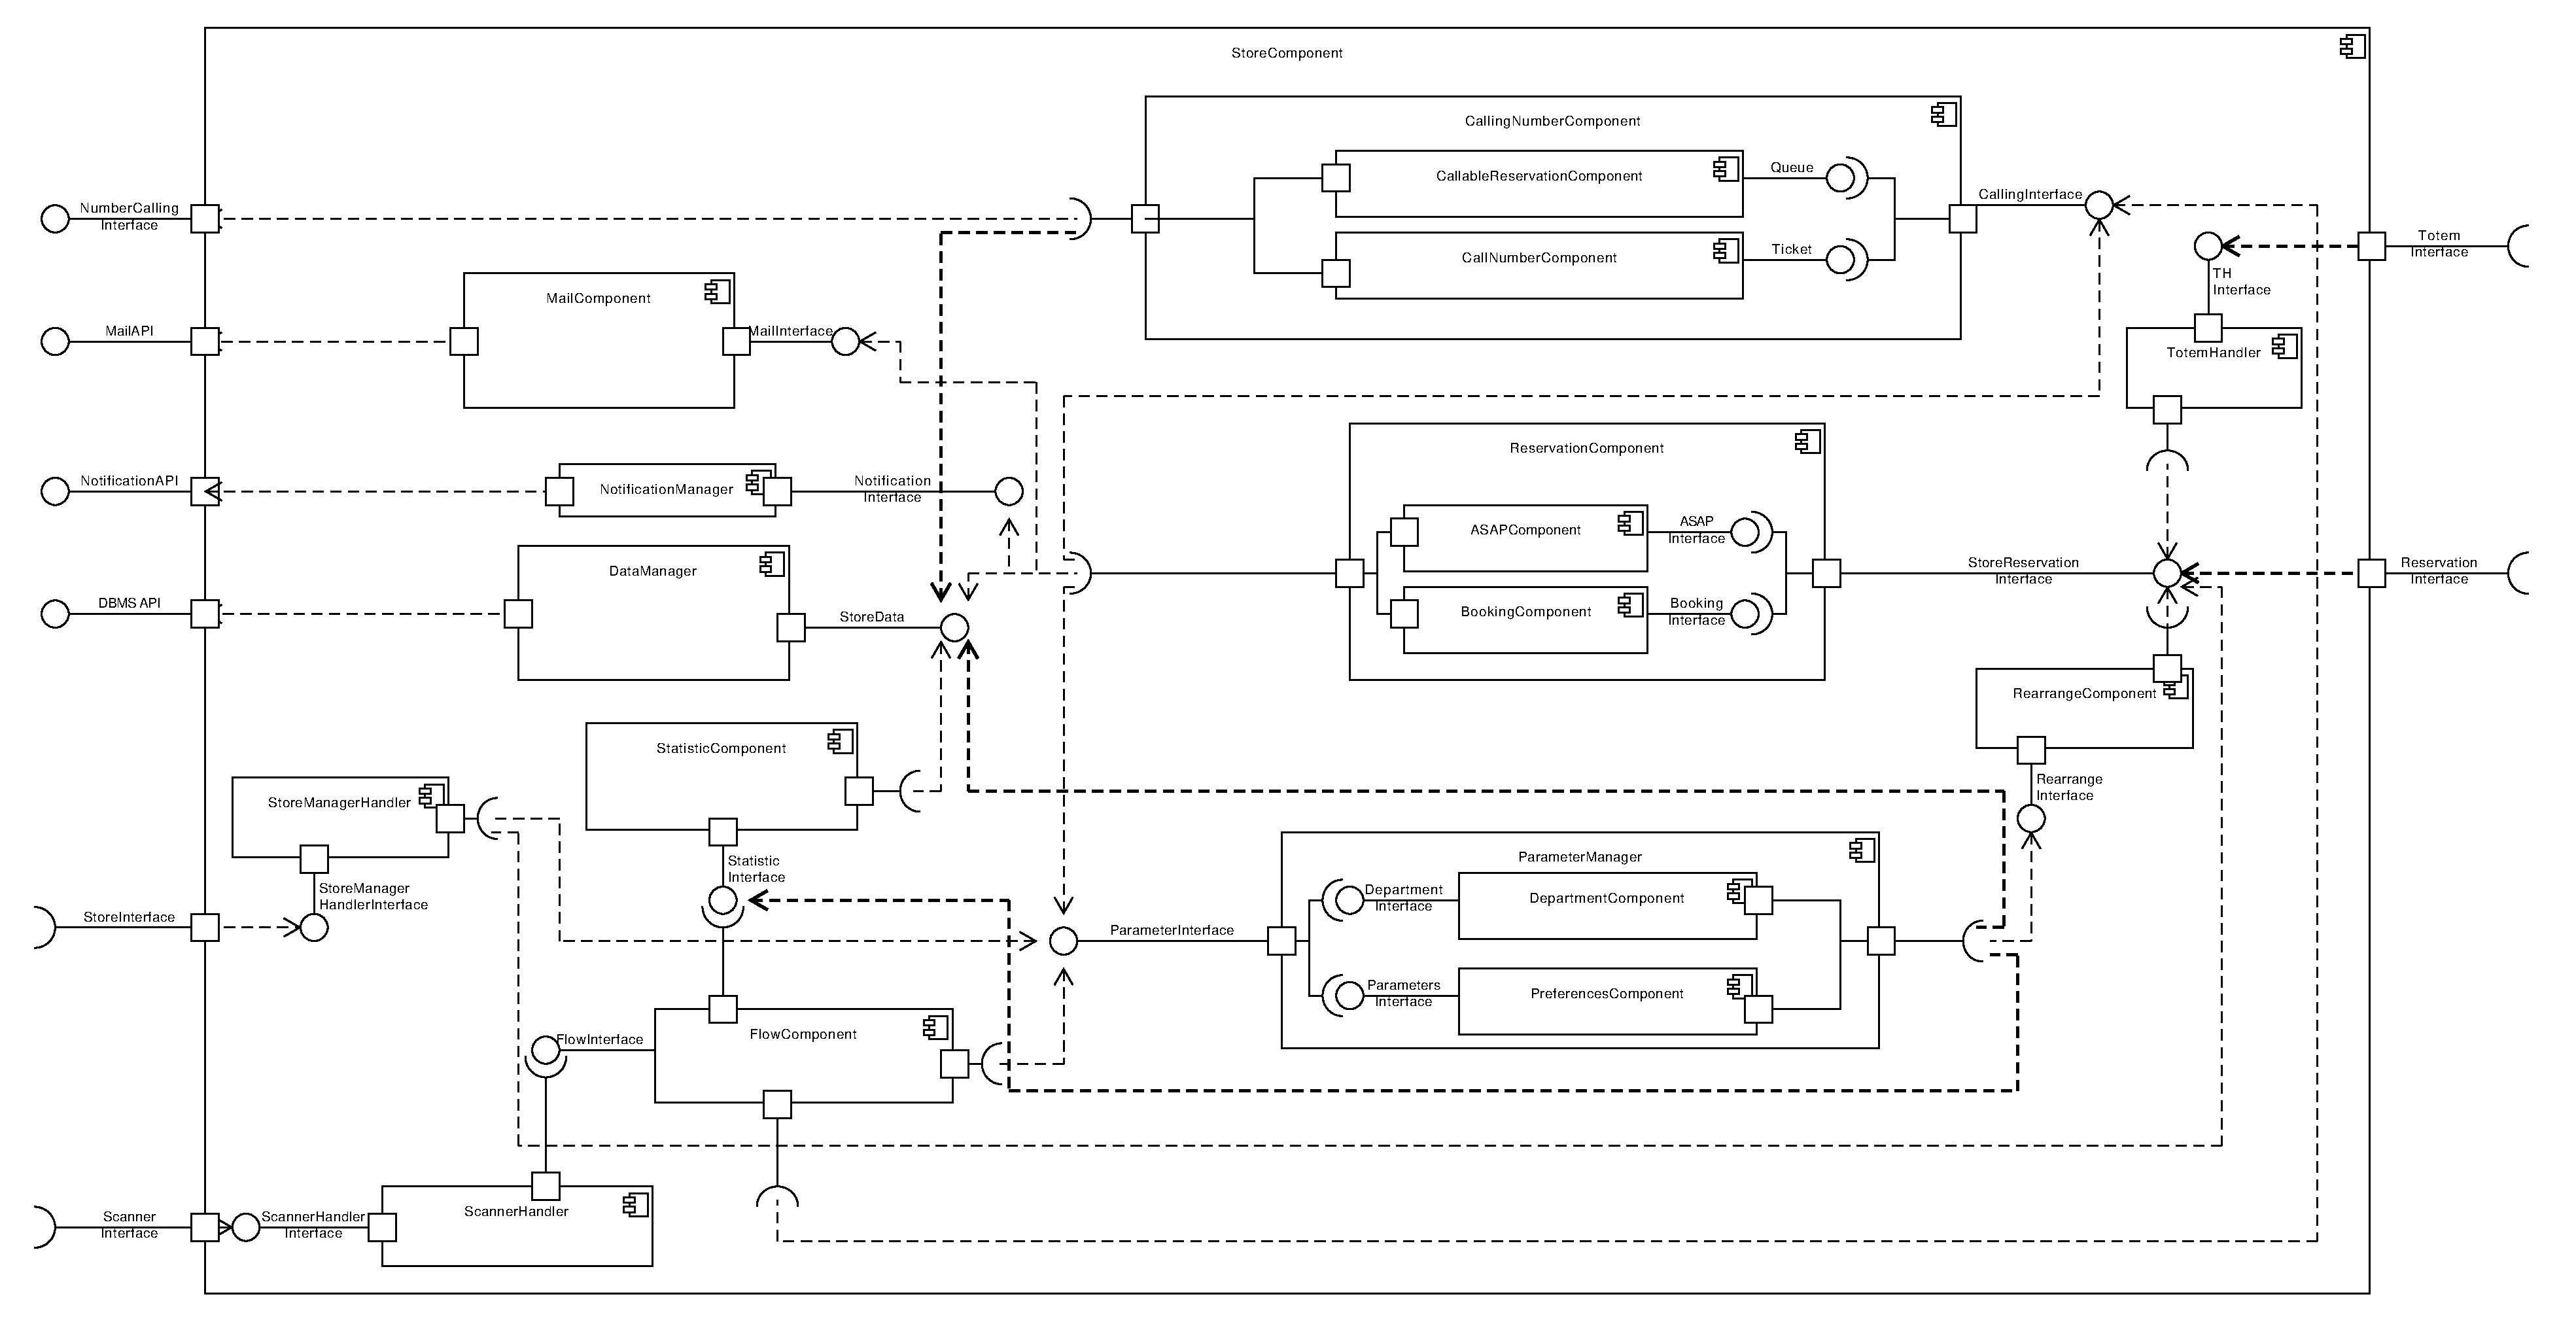
\includegraphics[scale=0.22, angle=90, trim= 0 0 0 -5cm]{Component Diagrams/ReorderedStoreComponentView.pdf}\\
				\end{adjustwidth}
				\caption{\emph{Store Component View}}
			\end{figure}
			\newpage
			
		\subsubsection{Store Manager Handler Component}
			The Store Manager Handler is the component that manages all the actions that a store manager can make within the application. The component analyzes various aspects:
			
			\begin{itemize}
				\item Reservations
				\item Modify Parameters
			\end{itemize}
		
			This component handles all the possible settable options of a store manager, it is invoked on the \emph{StoreInterface}, from the mobile application, and it interfaces with \emph{StoreComponentInterface}, that manages all information regarding parameters and reservations.
			
			\begin{itemize}
				\item {\bfseries ManagerReservationHandler}: it is the component that manages the store reservations and it is divided in two sub-component:
				
				\begin{itemize}
					\item {\bfseries DeleteRes}: it is the component that manages the elimination of the reservations.
					\item {\bfseries ModifyRes}: it is the component that manages the modification of the reservations.
				\end{itemize}
				
				\item {\bfseries ModifyParameters}: it is the component that manages the store parameter. They are of two types:
				
				\begin{itemize}
					\item {\bfseries DepartmentManager}: it is the component that manages all the parameters which concern the individual departments. Indeed, the store manager can add or delete a new department and can modify the maximum capacity of each department.
					\item {\bfseries StoreSettingManager}: it is the component that manages all the parameters which concern the entire store. Indeed, the store manager, can change the maximum capacity of the people inside the store and can modify the opening and closing hours.
				\end{itemize}
			
				\item {\bfseries RetrieveReservation}: it is the component that manages all the reservation of a specific store.
				
				\item {\bfseries SituationManager}: it is the component that manages the requests for the real time situation of the store.
			\end{itemize}
		
		\begin{figure}[H]
			\begin{adjustwidth} {-4cm}{}
				\centering
				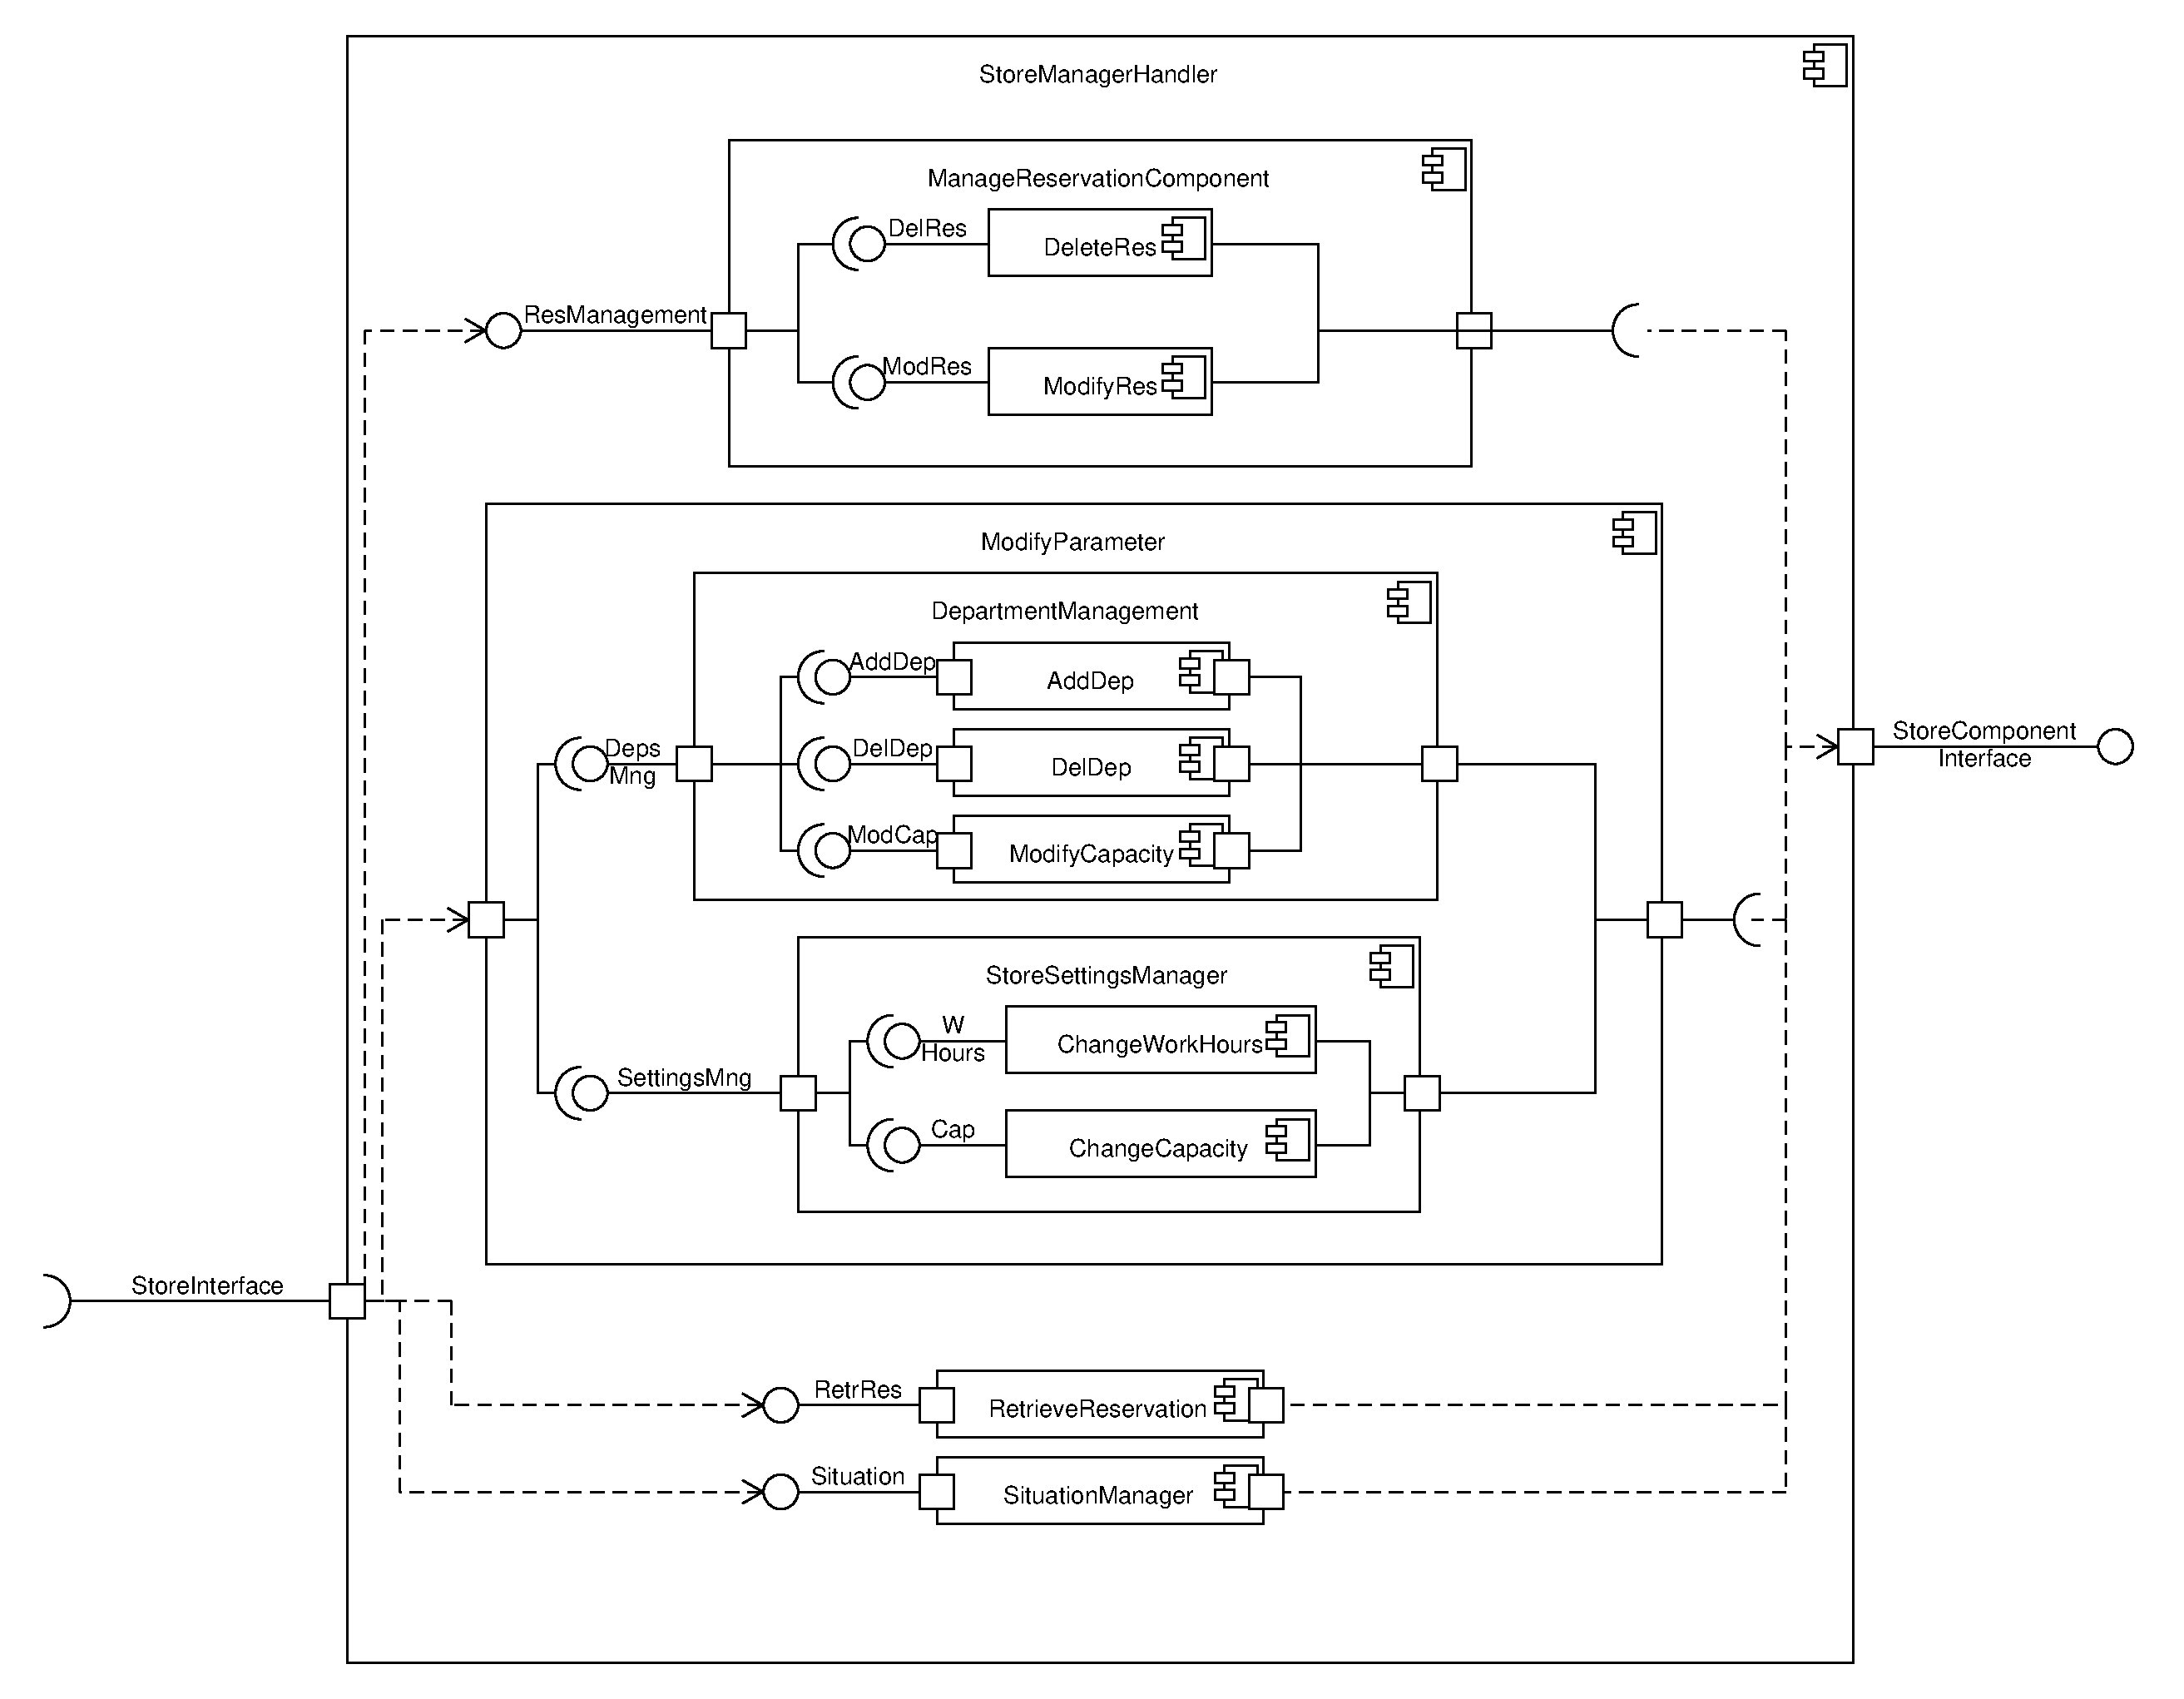
\includegraphics[scale=0.45]{Component Diagrams/StoreManagerHandlerComponentView.pdf}\\
			\end{adjustwidth}
			\caption{\emph{Store Manager Handler Component View}}
		\end{figure}
		\newpage
	\subsection{Deployment View}
	As said in the previous pages, the system have been developed in a very modular way, trying to handle all the required functionalities through dedicated components.\\
	Since the application needs to remotely communicate with various actor, the architecture which best fit for \emph{CLup} purposed is the {\bfseries client-server} one. Moreover, this architecture has been implemented through the {\bfseries three-tier} paradigm. This aims to separate the different logic part of the system: {\bfseries presentation}, {\bfseries business} and {\bfseries data}.
	\subsubsection{Client-side}
	In \emph{CLup}, there are many actors constituting the system's clients, since they are necessary for many \emph{CLup}'s features:
	\begin{itemize}
		\item {\bfseries Mobile App}: it's the mobile application used by \emph{customers} and \emph{store managers} to request services to \emph{CLup}. It also represents the {\bfseries Presentation tier} of the system, developed following the \emph{thin client} paradigm, leaving the whole business logic to the server, but for a thing: the notifications when a customer should depart for the store, and the map related functions. In fact, it's the \emph{Mobile App} that monitors when a it's time to go to the store. Even if a \emph{thin client} shouldn't handle operations, this aims to reduce the work load of the server: it's useless to remotely request the customer's position, and then send it to the \emph{Map Service}, while mobile devices can do it on their own (the same applies for distance and travel time);
		\item{\bfseries QR Code Scanner}: it's role is to send server the scanned \emph{QR Code} to process it;
		\item{\bfseries Totem}: a client needed to allow making requests at any store;
		\item{\bfseries Number Calling Device}: it's the device used to receive from the server the called reservations, so that a customer in front of the store knows when they can enter.  
	\end{itemize}
	\subsubsection{Server-side}
	\emph{CLup}'s server side implements both {\bfseries business logic} and {\bfseries data logic}.
	\begin{itemize}
		\item {\bfseries Business-logic}: it's implemented by {\bfseries CLupServer} and {\bfseries StoreComponent}. The first is needed to manage users access to \emph{CLup} services, and to manage reservations request, forwarding them to the correct store, or to generate suggestions querying all the store managed by the system. Instead, \emph{StoreComponent} manages the business logic related to each store, including reservations, ticket calling, capacity ecc. This design choice is to separate the logic of each store, and to avoid disservices to the whole \emph{CLup} system if something may fail.
		\item{\bfseries Data-logic}: it's implemented through various {\bfseries \emph{DBMS}}s: one for the general server, and one for each store. Business components can access the \emph{DBMS} though their related DataManager, the adapter between \emph{DBMS} and other components.
	\end{itemize}
	Here, follows a diagram of the subdivision of the various tiers. The clients (implementing the presentation tier) are in \textcolor{red}{red}, the components related to the business logic in \textcolor{blue}{blue}, while the data-related parts are in \textcolor{green}{green}.
	\bigskip
	\begin{figure}[H]
		\begin{adjustwidth} {-3cm}{}
			\centering
			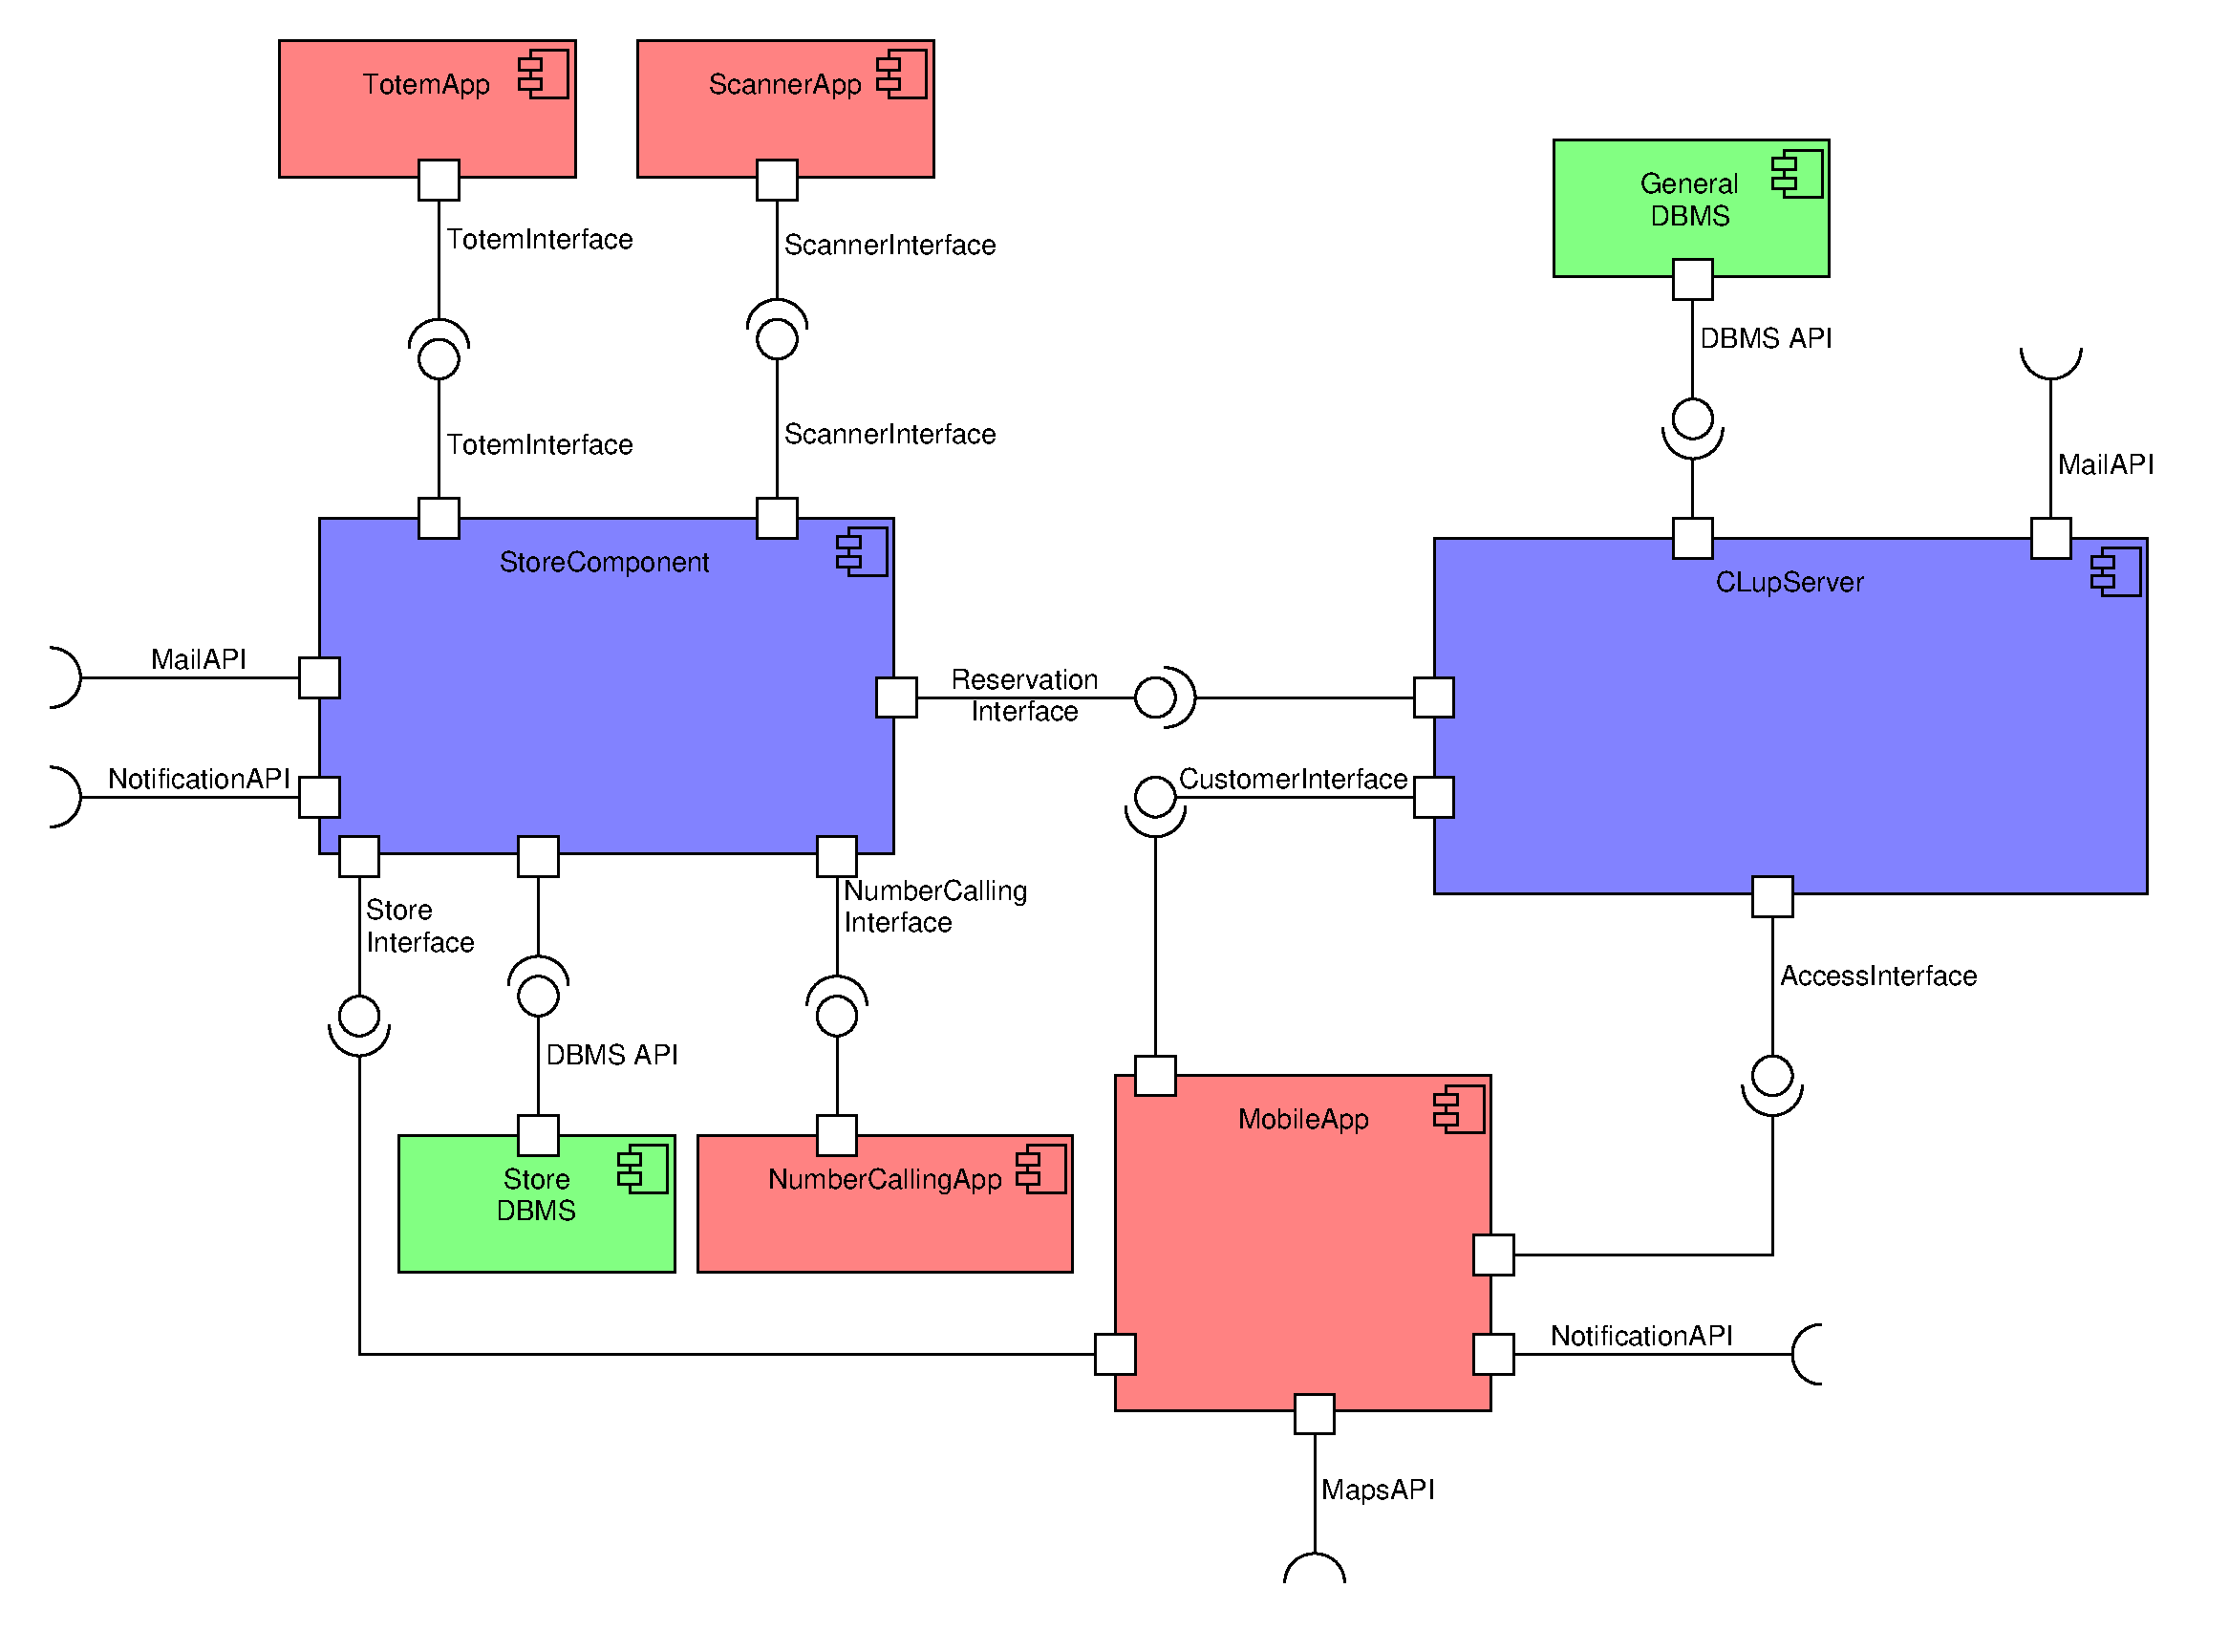
\includegraphics[scale=0.45]{Component Diagrams/ColorfulHighLevel.pdf}\\
		\end{adjustwidth}
		\caption{\emph{Component mapping with tiers}}
	\end{figure}
	\subsubsection{Deployment Diagram}
	Here there is the deployment diagram of the described system. As described in the \emph{RASD}, all the communications are routed via the \emph{TCP-IP} transmission protocol, using a secure transport protocol (such as \emph{TLS}). For example, \emph{HTTPS} may be used to connect client and server, and to access external services.
	
		\begin{figure}[H]
		\begin{adjustwidth} {-3cm}{}
			\centering
			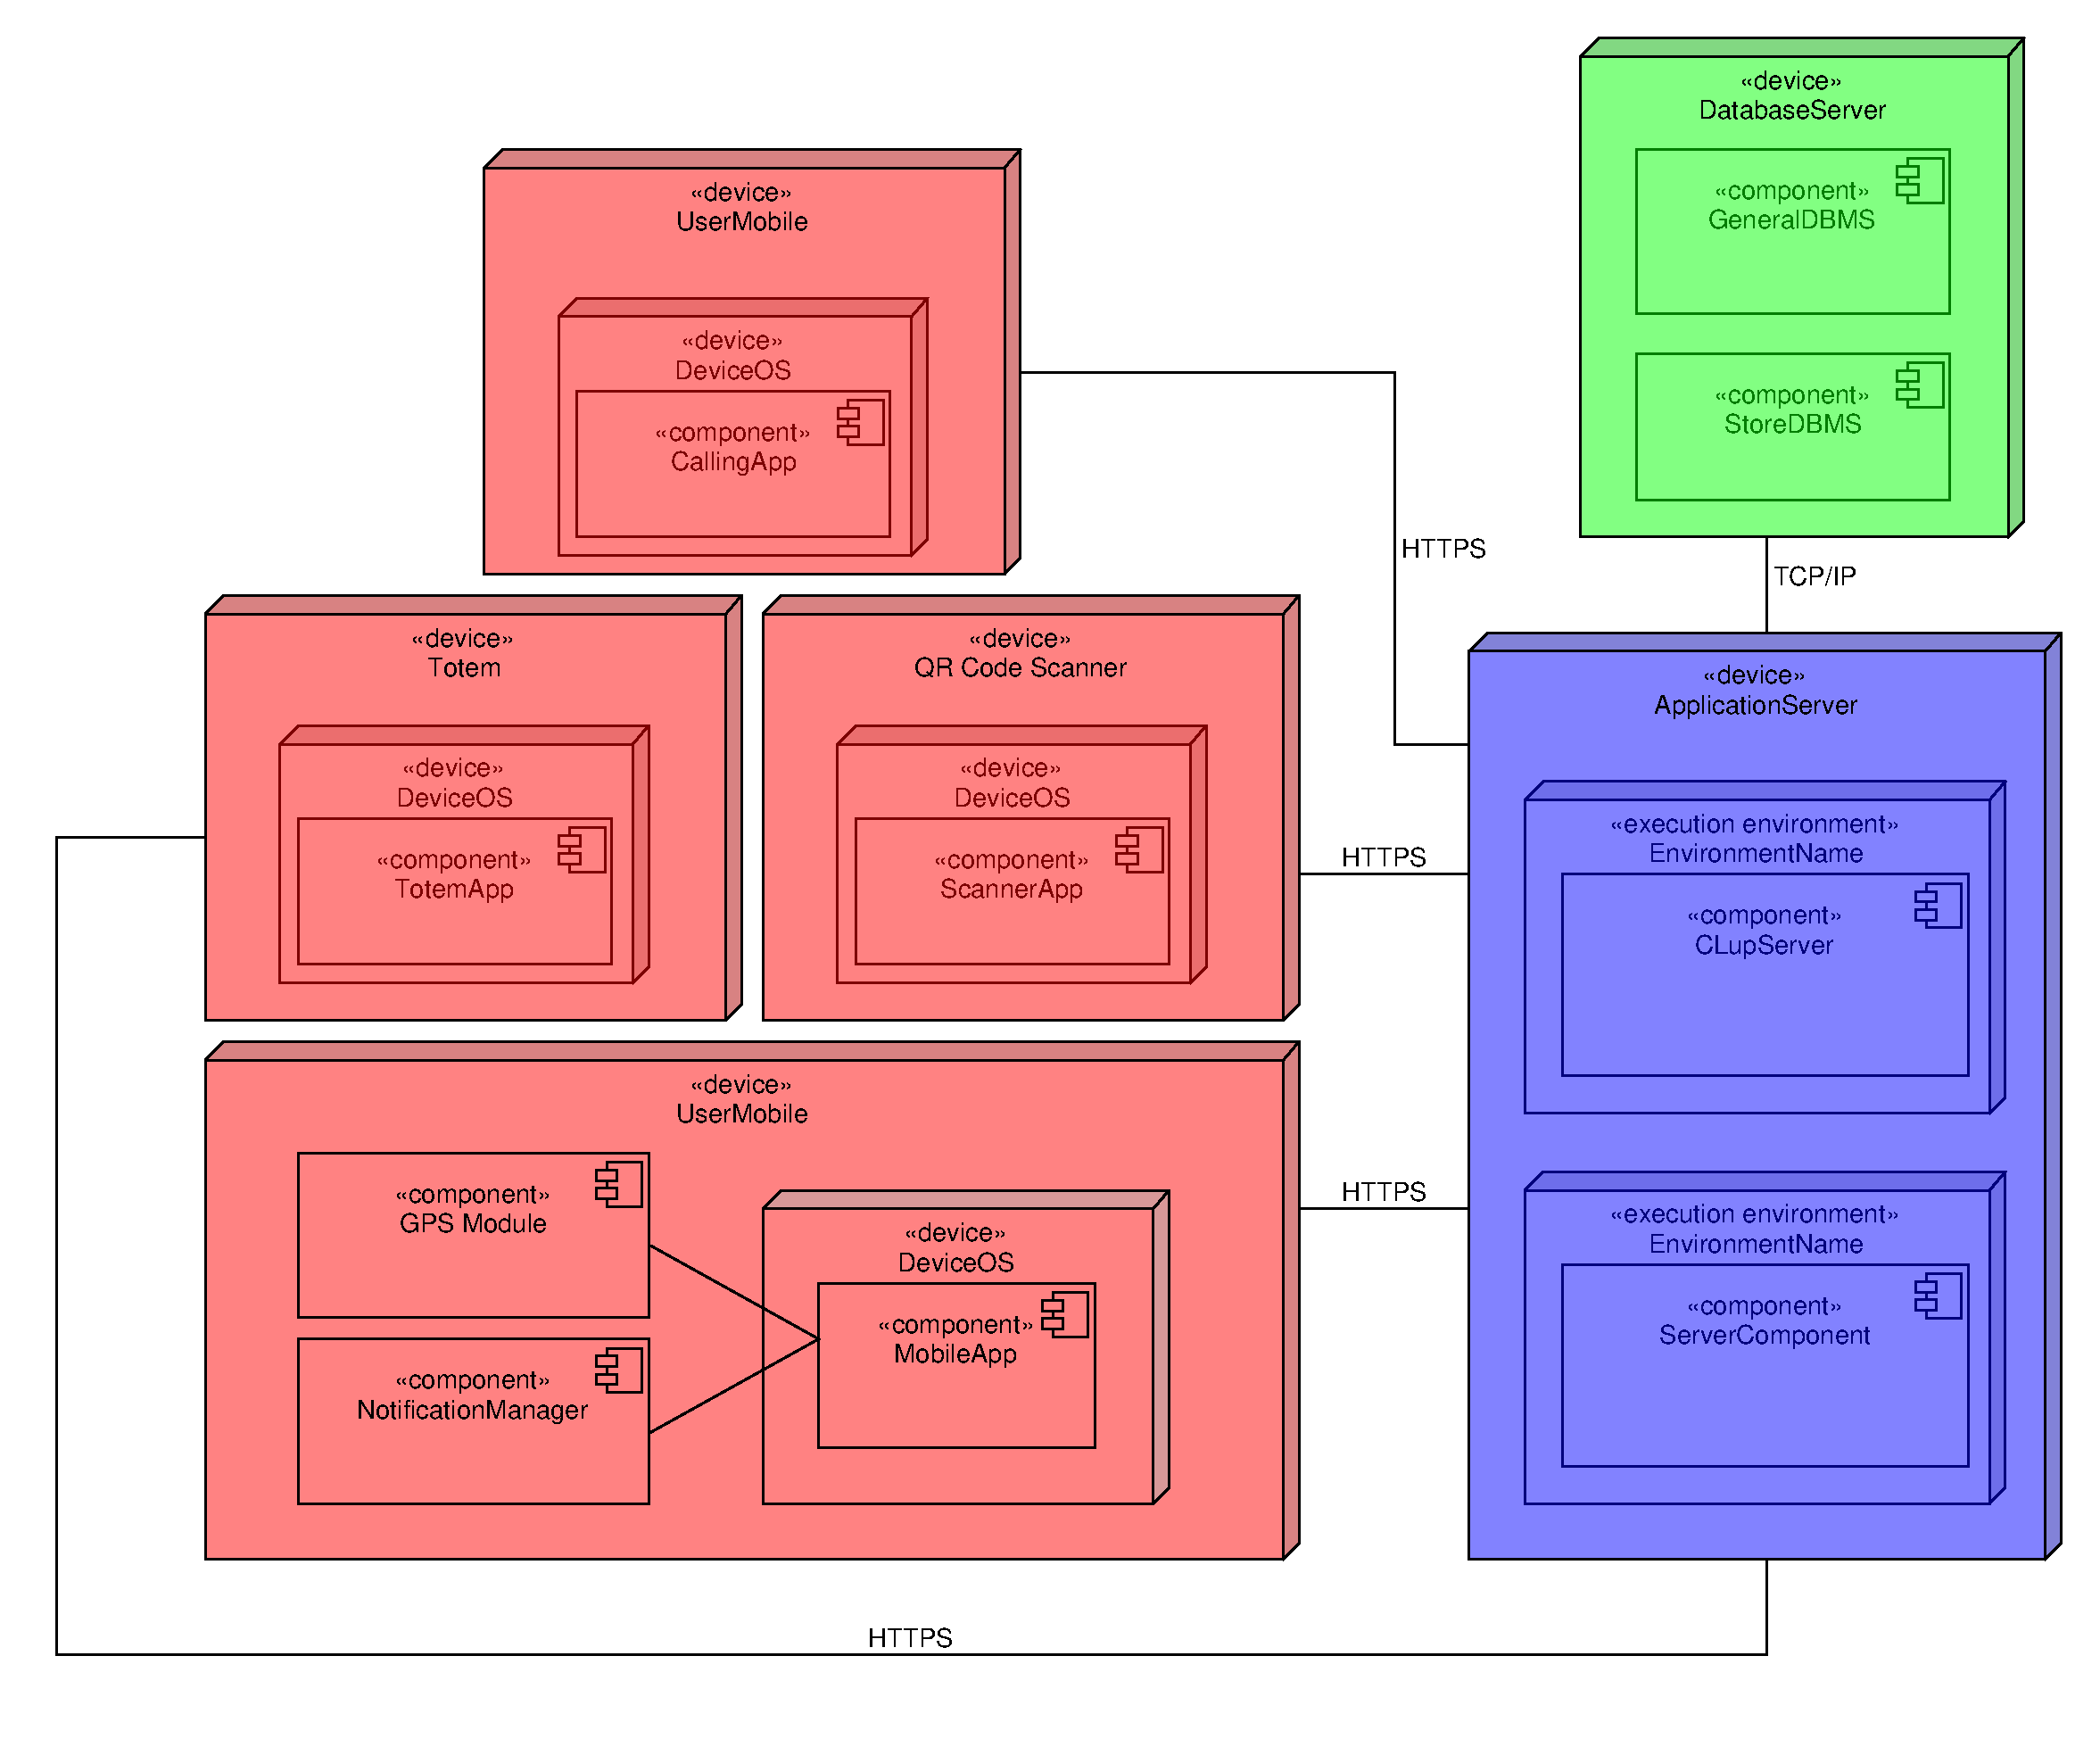
\includegraphics[scale=0.45]{Component Diagrams/DeploymentDiagram.pdf}\\
		\end{adjustwidth}
		\caption{\emph{Deployment Diagram}}
	\end{figure}
	
	
	\subsection{Runtime View}
	In this section will be analysed the runtime view of the system, through some \emph{Sequence Diagrams}. This should help to understand how the different components interact. Some aspects have been simplified to make the diagrams more readable; e.g., some interactions with the \emph{DBMS} and between adapters and external services have been omitted, some operations with identical behaviour have been collapsed in generic requests, through a generic method, just to model the interaction. The \emph{Component Interfaces diagram} will report all these methods in detail.
	\subsubsection{User login}
	 Since the interactions for both \emph{customers} and \emph{managers} log-in are the same, here there is reported only the ones relative to customers.
	
	\begin{figure}[H]
		\begin{adjustwidth} {-0.6cm}{}
			\centering
			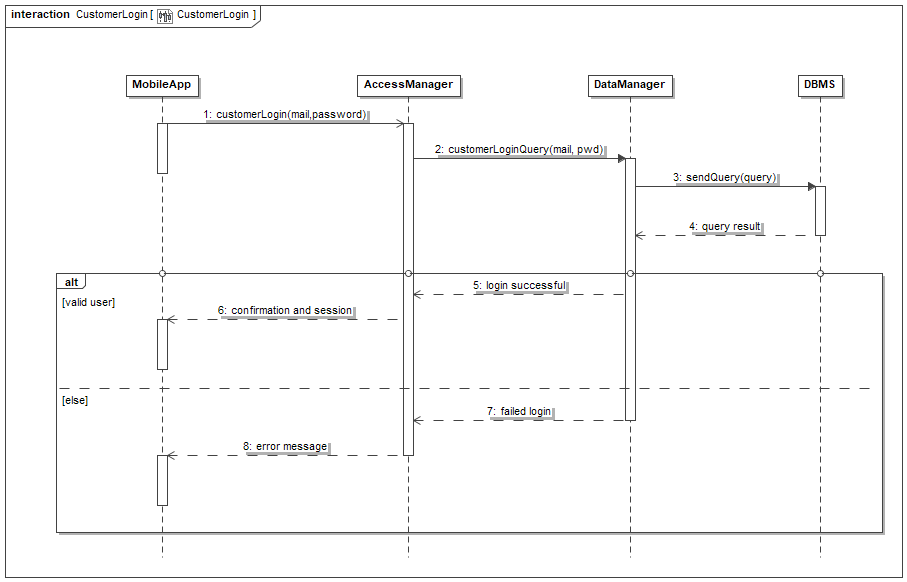
\includegraphics[scale=0.4]{Sequence Diagrams/sd__CustomerLogin__CustomerLogin.png}
		\end{adjustwidth}
		\caption{\emph{Customer Login Sequence Diagram}}
	\end{figure}

	First of all, the {\bfseries Mobile App} requests the {\bfseries Access Manager} to check the credentials. This is done by asking the {\bfseries Data Manager} to query the \emph{DBMS} for the selected credentials. Once the operations on \emph{DBMS} ended, the {\bfseries Access Manager} will send an error message if the credentials are not valid, or a confirmation. Then, in the latter case, AccessManager forwards the user's session. If it's a manager to log-in, the {\bfseries MobileApp} will use the \emph{StoreManagerLogin} method, passing as parameter the \emph{StoreID} instead of the \emph{email}.
	
	\subsubsection{Customer Registration}
		\begin{figure}[H]
		\begin{adjustwidth} {-3.5cm}{}
			\centering
			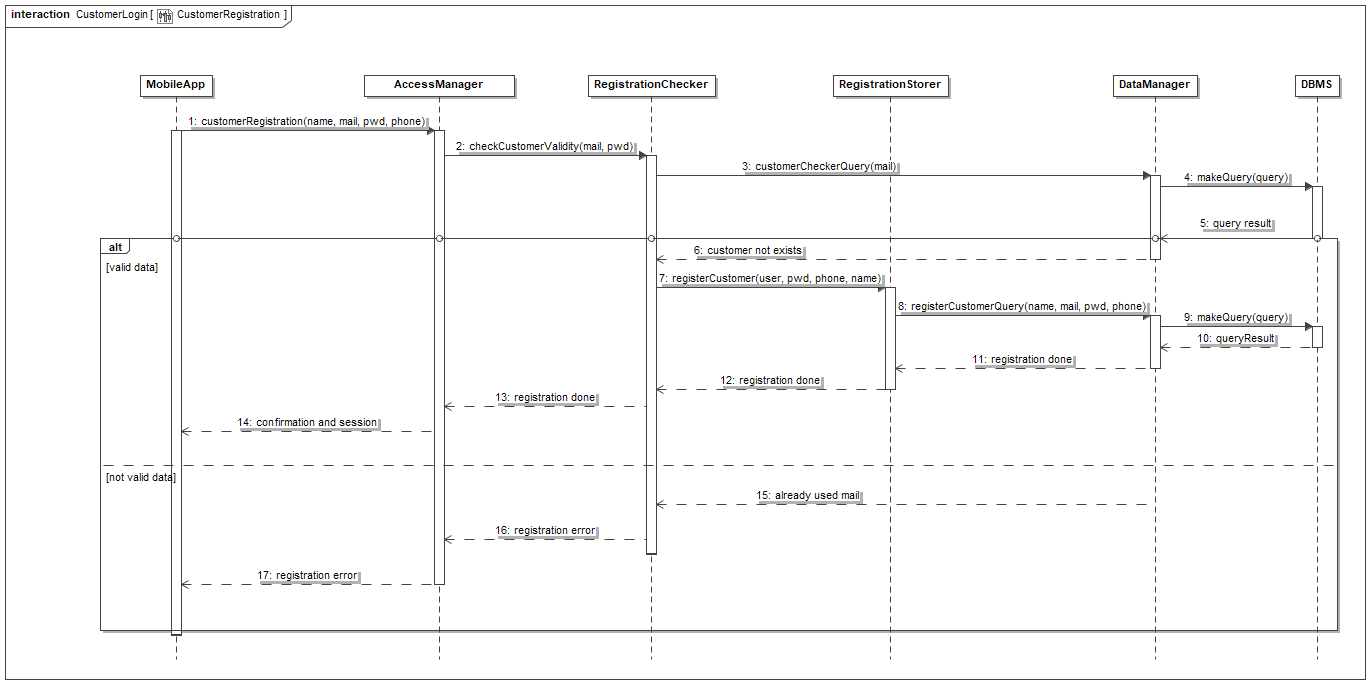
\includegraphics[scale=0.4]{Sequence Diagrams/sd__CustomerLogin__CustomerRegistration.png}
		\end{adjustwidth}
		\caption{\emph{Customer Registration Sequence Diagram}}
	\end{figure}
	
	The registration process for a customer is quite similar to the login one. In fact, the app requests the {\bfseries AccessManager} to register the customer with the inserted data. Then a request to check the selected credentials is forwarded from the {\bfseries RegistrationChecker} to the {\bfseries DataManager} . If the selected email isn't already in the system, the registration process continues, and the user is stored in the \emph{DBMS}; at the end, the \emph{MobileApp} receives the confirmation and the session. If the credentials are not valid, an error message is sent.
	
	\subsubsection{Store Manager Registration}
	The registration process for a \emph{Store Manager} is identical to \emph{customers} one, but for the intermediate step of certification check. In fact, if the credentials are valid, before registering the user, the {\bfseries RegistrationChecker} verify the validity of the uploaded certification. If valid, the process continue, else an error message is thrown to the {\bfseries MobileApp}.
	\begin{figure}[H]
		\begin{adjustwidth} {-3cm}{}
			\centering
			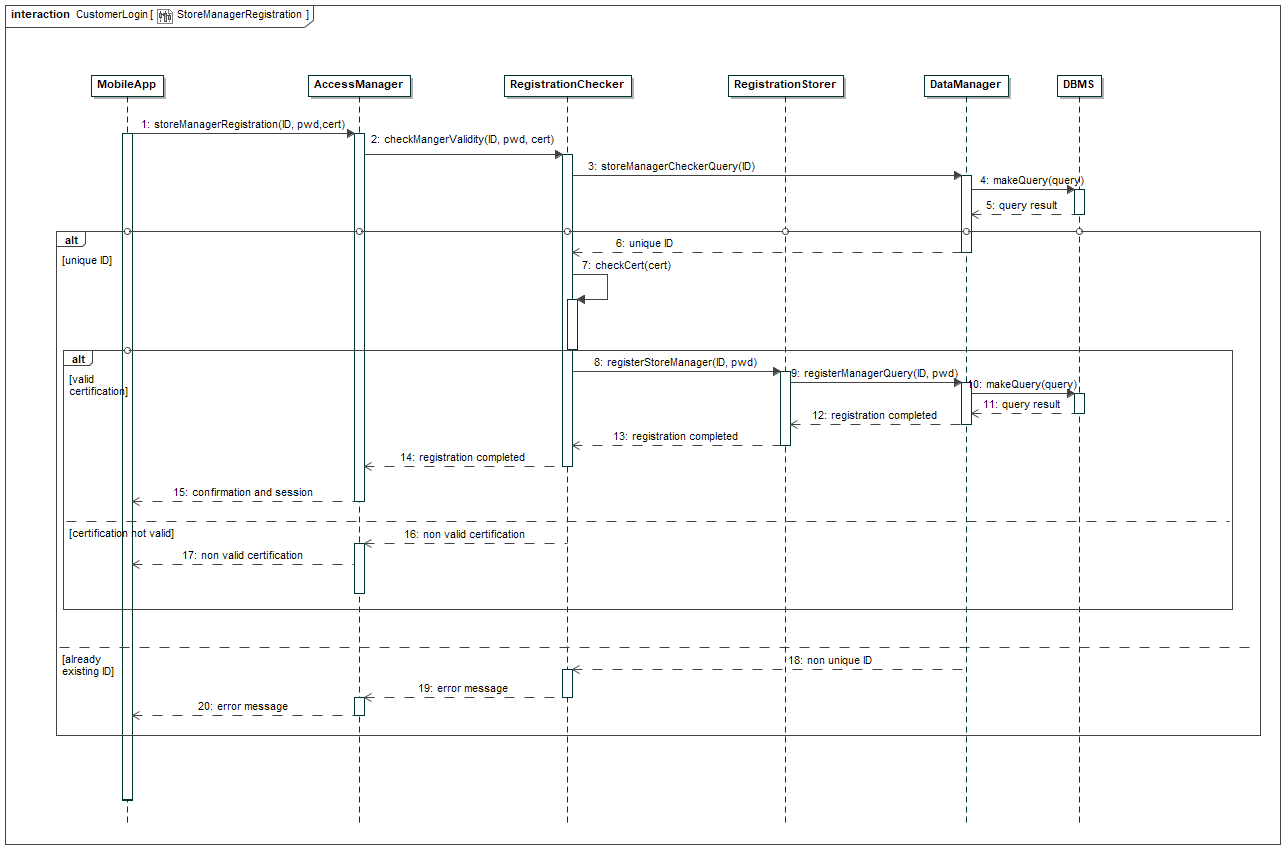
\includegraphics[scale=0.4]{Sequence Diagrams/sd__CustomerLogin__StoreManagerRegistration.png}
		\end{adjustwidth}
		\caption{\emph{Store Manager Registration Sequence Diagram}}
	\end{figure}
	
	\subsubsection{Make a reservation}
	To make a \emph{reservation}, it's necessary to retrieve the list of stores. So, through the {\bfseries CustomerHandler}, the {\bfseries MobileApp} requests to the {\bfseries ReservationHandler} the list of stores. Once retrieved from the \emph{DBMS}, this list is sent to the {\bfseries MobileApp} and sorted by distance, through the \emph{Map Service}.
	Then, after the customer select the store, the departments, and insert the shopping time estimation (here it's not treated the calculation by the \emph{CLup} for the sake of simplicity), they can both make an \emph{ASAP reservation}, or a \emph{Booking}.
	\begin{figure}[H]
		\begin{adjustwidth} {-1cm}{}
			\centering
			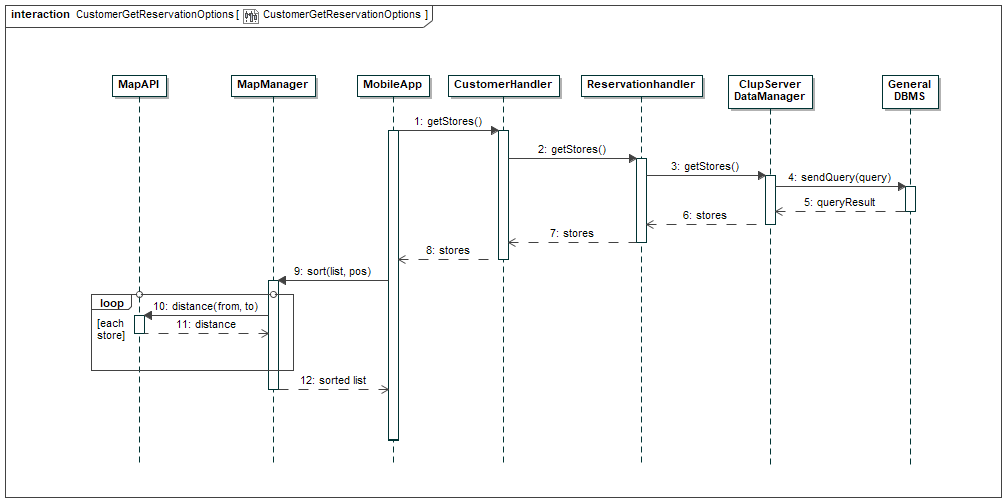
\includegraphics[scale=0.4]{Sequence Diagrams/sd__CustomerGetReservationOptions__CustomerGetReservationOptions.png}
		\end{adjustwidth}
		\caption{\emph{Reservation Options Sequence Diagram}}
	\end{figure}

	
	\begin{figure}[H]
		\begin{adjustwidth} {-1.5cm}{}
			\centering
			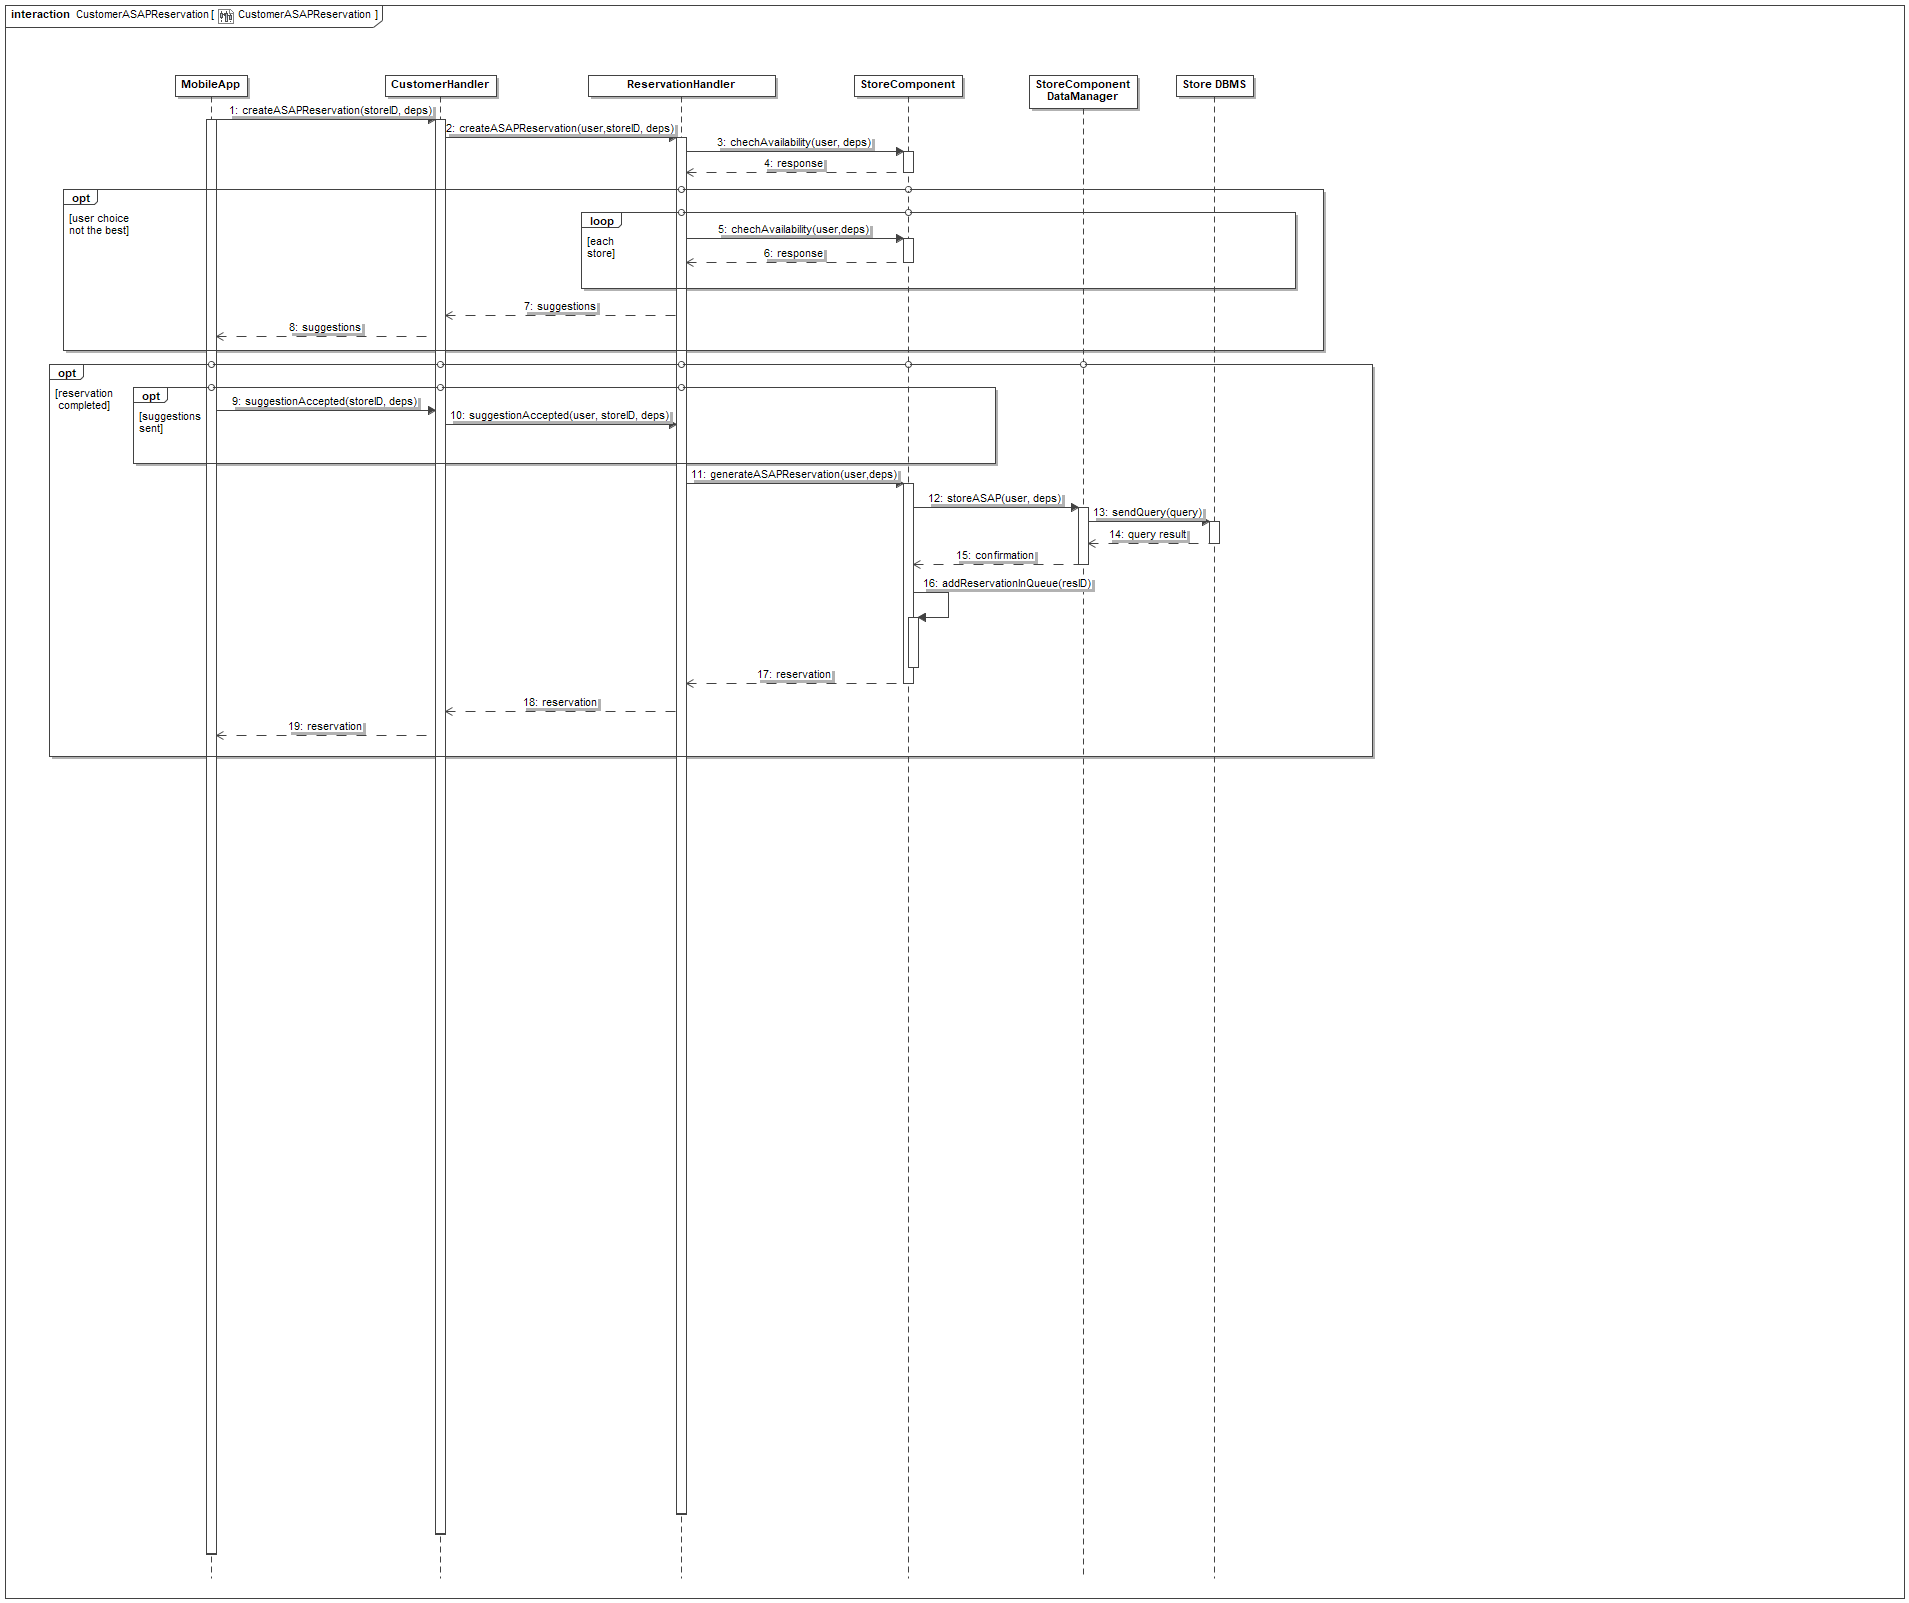
\includegraphics[scale=0.3]{Sequence Diagrams/sd__CustomerASAPReservation__CustomerASAPReservation.png}
		\end{adjustwidth}
		\caption{\emph{ASAP Reservation Sequence Diagram}}
	\end{figure}
	In the case of an ASAP reservation, a request is sent to the {\bfseries ReservationHandler}, that asks to the component of the selected store if the reservation is possible, with the eventual waiting time. In the case the user choice is ok and optimal, the {\bfseries Store Component} receives the request to save the reservation, and after queueing it, the ticket is sent to the customer; else, some \emph{suggestions} are generated and sent to the customer, who can choose among them. After an option have been selected, it starts the previously described process.\\\\
	Instead, if the customer desire to make a \emph{booking}, the {\bfseries ReservationHandler} asks the selected store's {\bfseries StoreComponent} when the customer can enter the store, and forward it to the {\bfseries MobileApp}. Then, the time intervals are shown to the customer. If they're not satisfied with the proposed options, it's possible to ask for suggestion. So, the {\bfseries ReservationHandler} queries all the stores for time intervals, and send them back to the MobileApp. So, the customer can select a store, and see its time intervals. When they are satisfied, select a time interval and confirm the selection. The request arrives at the {\bfseries StoreComponent}, that, if the selection is correct, creates the \emph{reservation}, puts it in queue and forward to the customer. If the selection is wrong, an error message is sent to the {\bfseries MobileApp} and the time interval page is reloaded.
	\bigskip
	
	\begin{figure}[H]
		\begin{adjustwidth} {-1cm}{}
			\centering
			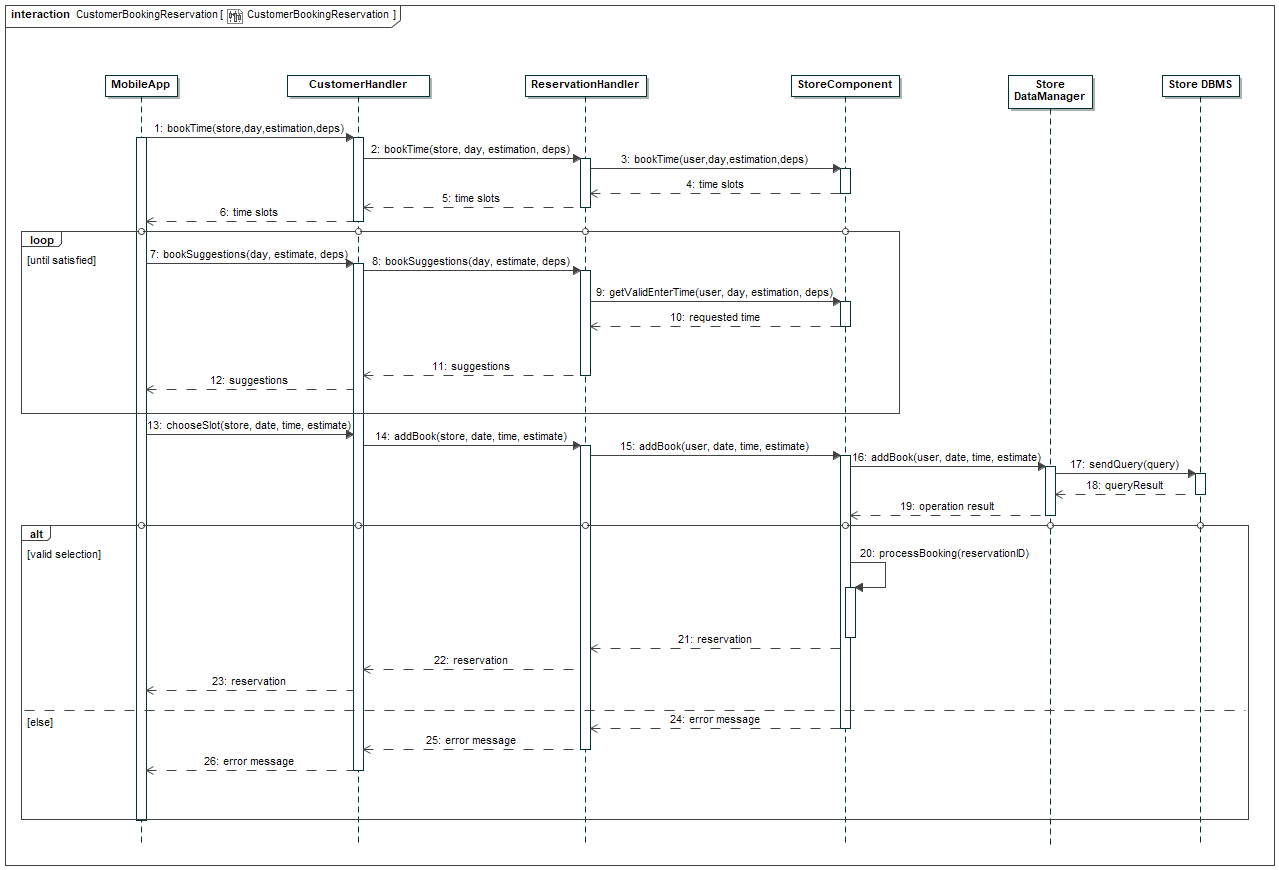
\includegraphics[scale=0.3]{Sequence Diagrams/sd__CustomerBookingReservation__CustomerBookingReservation.png}
		\end{adjustwidth}
		\caption{\emph{Book Reservation Sequence Diagram}}
	\end{figure}

	\subsubsection{Customer Reservations Handling}
	\emph{CLup} allows customers to retrieve and manage their reservations from the \emph{Mobile App}. When a reservation is opened from the personal area on the app, its details (such as \emph{ETA} to enter the store and the needed time to get physically at the building) are updated.
	\begin{figure}[H]
		\begin{adjustwidth} {-1cm}{}
			\centering
			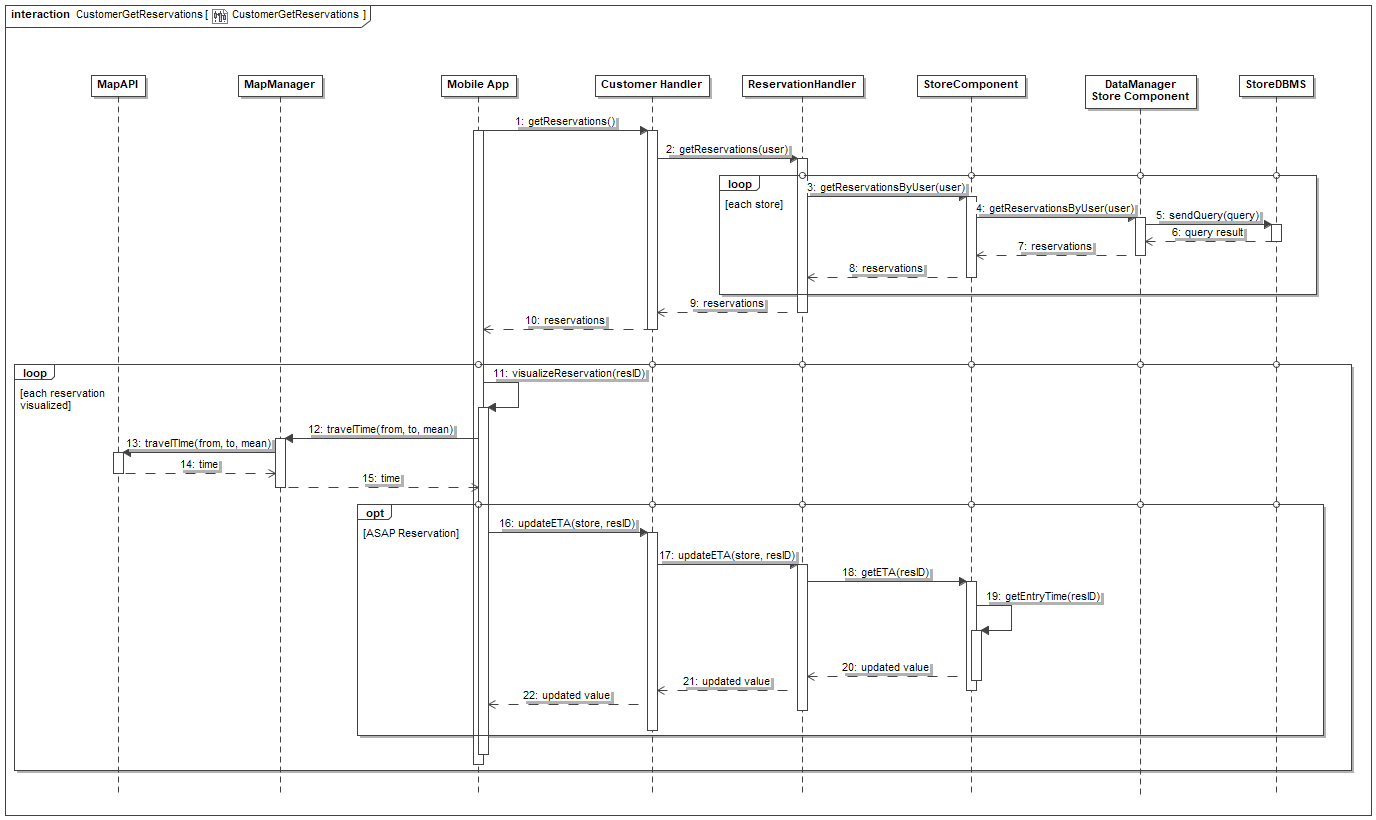
\includegraphics[scale=0.3]{Sequence Diagrams/sd__CustomerGetReservations__CustomerGetReservations.png}
		\end{adjustwidth}
		\caption{\emph{Get Reservations Sequence Diagram}}
	\end{figure}
	When the customer open the app's area reserved for made reservations, and there is an internet connection, the \emph{Mobile App} requests the server for all the reservations made by the logged customer; the process is mainly handled by the ReservationHandler, that queries all the stores for the reservations. Once this process is completed, the customer have a list of reservations. When someone is opened, the app requests the travel time for the store to the MapManager, and, in case of an \emph{ASAP} reservation, the new \emph{ETA} to enter the store at the ReservationHandler (which forward the request to the correct store component).\\\\
	In the following diagram there are modelled the interactions occurring when a reservation is modified; the diagram is simplified, since each specific operation (such as delete, reschedule ecc.) are substituted by a generic ModifyReservations; that's not a problem, since the interactions are the same for all type of operation.
	When the related store's {\bfseries ReservationComponent} receives the modification request, process it, register it in the \emph{DBMS} and notify the {\bfseries CallingNumberComponent} of the modification, so that the queue can be accordingly updated.
	\begin{figure}[H]
		\begin{adjustwidth} {-0.8cm}{}
			\centering
			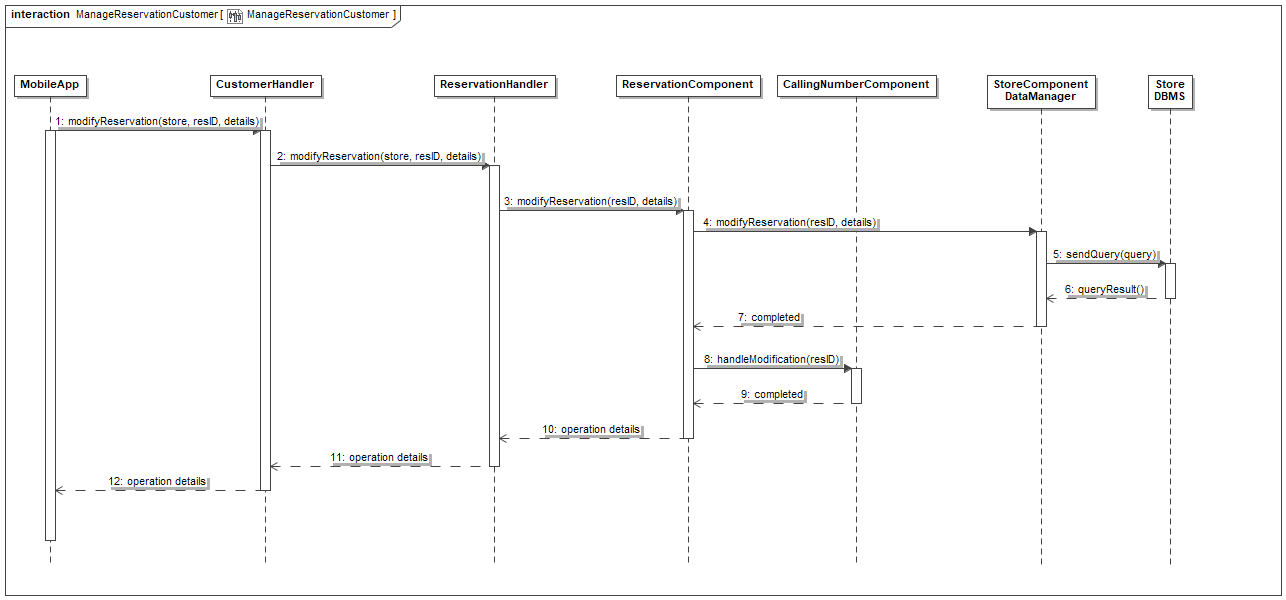
\includegraphics[scale=0.3]{Sequence Diagrams/sd__ManageReservationCustomer__ManageReservationCustomer.png}
		\end{adjustwidth}
		\caption{\emph{Reservation Modification Sequence Diagram}}
	\end{figure}

	\subsubsection{Store Management}
	As done for the customer side, here there is described how the different components dialogue to allow a \emph{store manager} in managing their store.\\
	A note on these sequence diagram: to make them more compact, the interactions with the {\bfseries StoreManagerHandler} have been avoided, since it's only a redirector from the \emph{Mobile App} to the correct component of the {\bfseries Store Component}.\\
	First of all, all the reservations must be retrieved from the server. The request is received from the {\bfseries ReservationComponent}, that queries the \emph{DBMS} for all the made reservations. Once retrieved the store's reservation, a manger can both contact customers about a specific reservation, or modify one.\\\\
	In the first case, after inserting a message, a mail send is requested to the {\bfseries StoreComponent}'s {\bfseries MailManager}.\\\\
	In case of a modification, the request is sent to the {\bfseries ReservationComponent}. After the changes are registered in the \emph{DBMS}, the {\bfseries ReservationComponent} asks the {\bfseries CallingNumberComponent} to update the store's queue, and then a notification of the changes is sent to the customer. 
		\begin{figure}[H]
		\begin{adjustwidth} {-1cm}{}
			\centering
			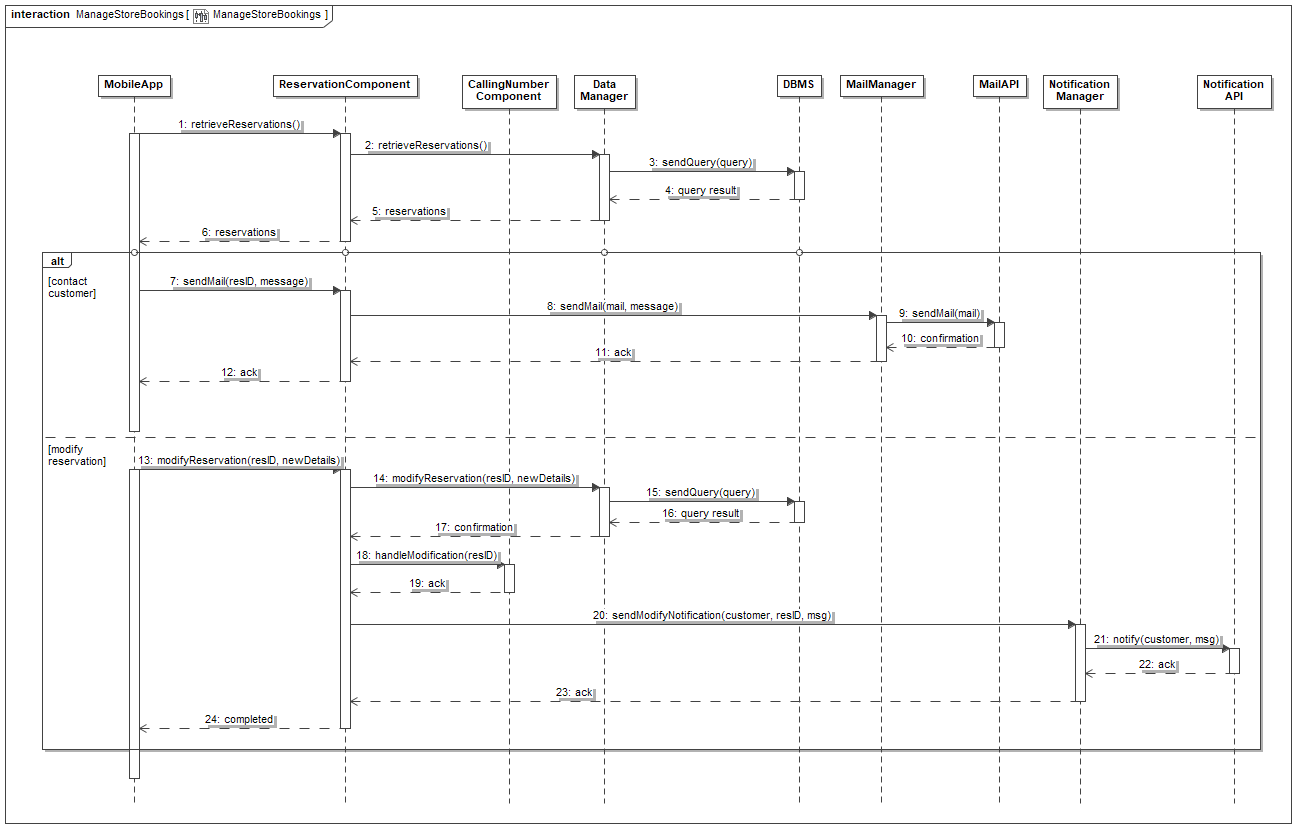
\includegraphics[scale=0.3]{Sequence Diagrams/sd__ManageStoreBookings__ManageStoreBookings.png}
		\end{adjustwidth}
		\caption{\emph{Store Manager Reservation Handling Sequence Diagram}}
	\end{figure}

	A store manager may also see the situation inside their store, among visits statistics. To do this, a request to the {\bfseries ParameterComponent} is made, that will query the \emph{DBMS} for the actual situation, the {\bfseries StatisticComponent} for the statistics, and finally send the data to the {\bfseries MobileApp}, that will elaborate them.

	\begin{figure}[H]
		\begin{adjustwidth} {-0.5cm}{}
			\centering
			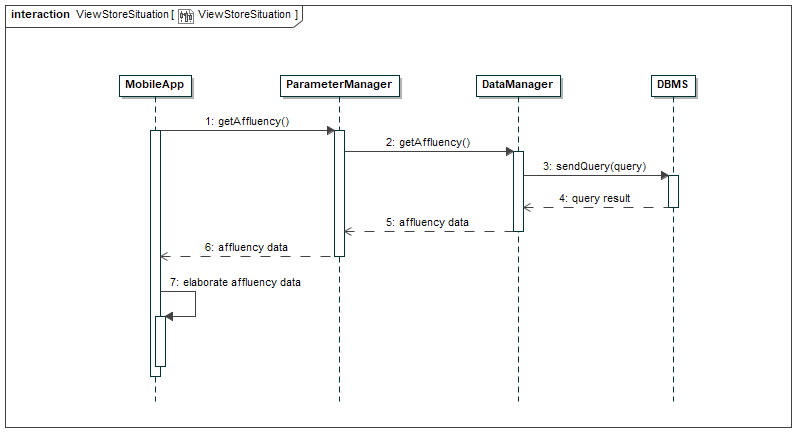
\includegraphics[scale=0.33]{Sequence Diagrams/sd__ViewStoreSituation__ViewStoreSituation.png}
			\end{adjustwidth}
		\caption{\emph{Monitor Store Situation Sequence Diagram}}
	\end{figure}
	\subsubsection{CLup Critical Features}
	In the previous sections, there are described the diagrams related to requests made by customers and store manager. But, \emph{CLup} also need to handle on its own some processes, needed to manage the store's flow.\\

	\begin{figure}[H]
		\begin{adjustwidth} {-1.2cm}{}
			\centering
			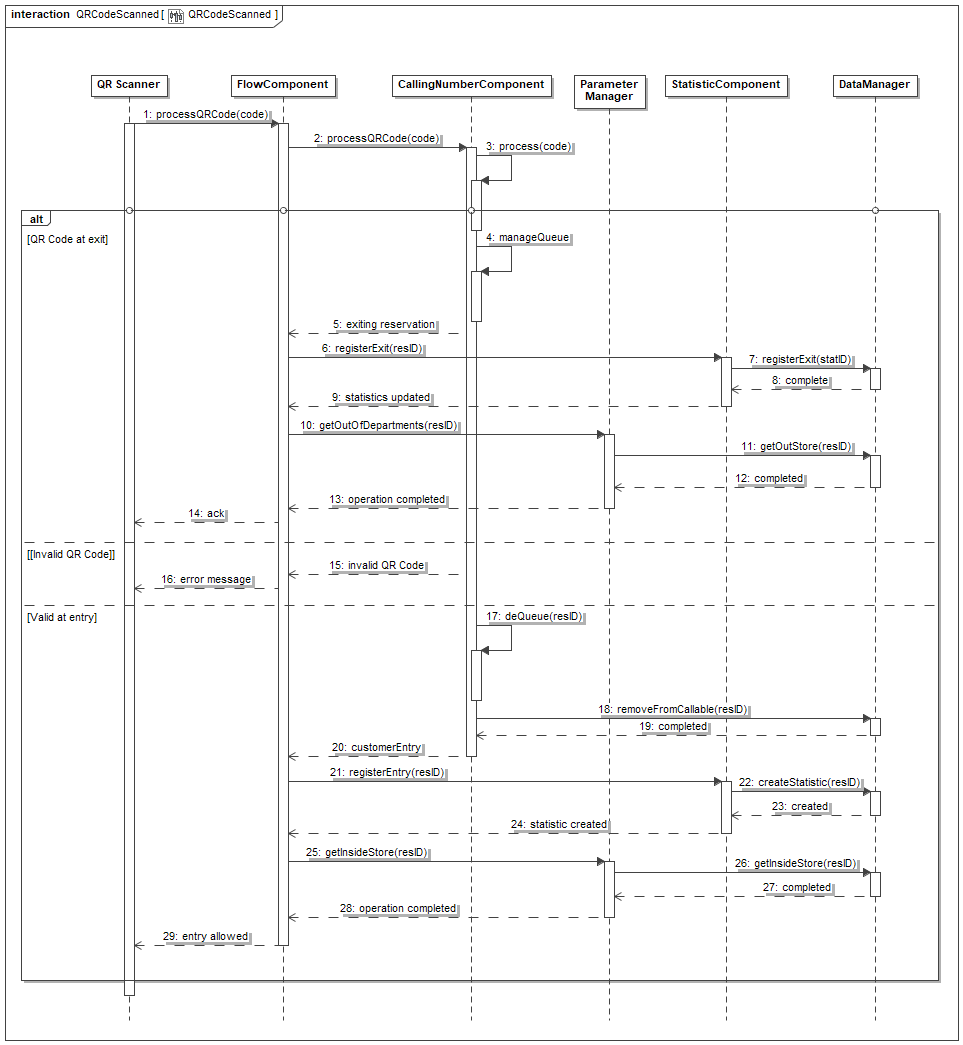
\includegraphics[scale=0.42]{Sequence Diagrams/sd__QRCodeScanned__QRCodeScanned.png}
		\end{adjustwidth}
		\caption{\emph{QR Code processing Sequence Diagram}}
	\end{figure}	
	In order to register customers' entry and exit, the scanned \emph{QR Code} must be processed. When a \emph{QR Code} is scanned, a request of processing is forwarded to the FlowComponent, that asks the CallingNumberComponent to check the status of the scanned \emph{QR Code}, and some case can happen:
	\begin{itemize}
		\item{\bfseries A customer exits the store}: in this case, the visit's statistics are updated through the StatisticComponent (that registers the exit in the \emph{DBMS}), and then the reservation is removed from the "inside" of the store, through a request to the ParameterManager (that updates the departments' status on the \emph{DBMS}). But, before returning the \emph{QR} status to the FlowComponent, the CallingNumberComponent starts the process to call a new number inside the store.
		\item{\bfseries Invalid QR Code}: a wrong \emph{QR Code} is scanned, and an error message sent to the store.
		\item{\bfseries Valid QR Code at entry} in this case, the CallingNumberComponent dequeues the reservation and notifies the FlowComponent of the \emph{QR} status. So, the visit statistics are generated and the customer put "inside the store", through the same components and dual requests used for the exit case. Finally, the authorization for entry is sent to the store. 
	\end{itemize}

	\subsubsection{Call A Number}
	Here there are described the actions made by the system to handle the process for calling a customer to get inside the store. This process is mainly triggered when the queue is modified in some way, such us someone exits the store, some reservation has been rescheduled or cancelled or someone didn't enter the store in time, and their reservation has been discarded. \\\\
	First of all, the CallingNumberComponent process the status of the queue, getting the first reservation that has the right to be called. Then, the ParameterManager is asked for the current situation of the store, and the data are sent back. In case there is the possibility to allow the considered customer to enter the store, the reservation is set as called called, this status registered in the \emph{DBMS}, and the call is notified to the NumberCallingApp, so that outside the store the number can be called. Finally, the system checks if the \emph{ETA} for some future reservation decreased, and if so sends a notification to the related customer's \emph{Mobile App}, so that the calculation of the departure time is precise. Even if not described in other diagrams, this last process takes place each time a modification in the queue is done.\\\\
	This process takes runs until the store is full and/or no other reservation can enter the store.

	\begin{figure}[H]
		\begin{adjustwidth} {-1.8cm}{}
			\centering
			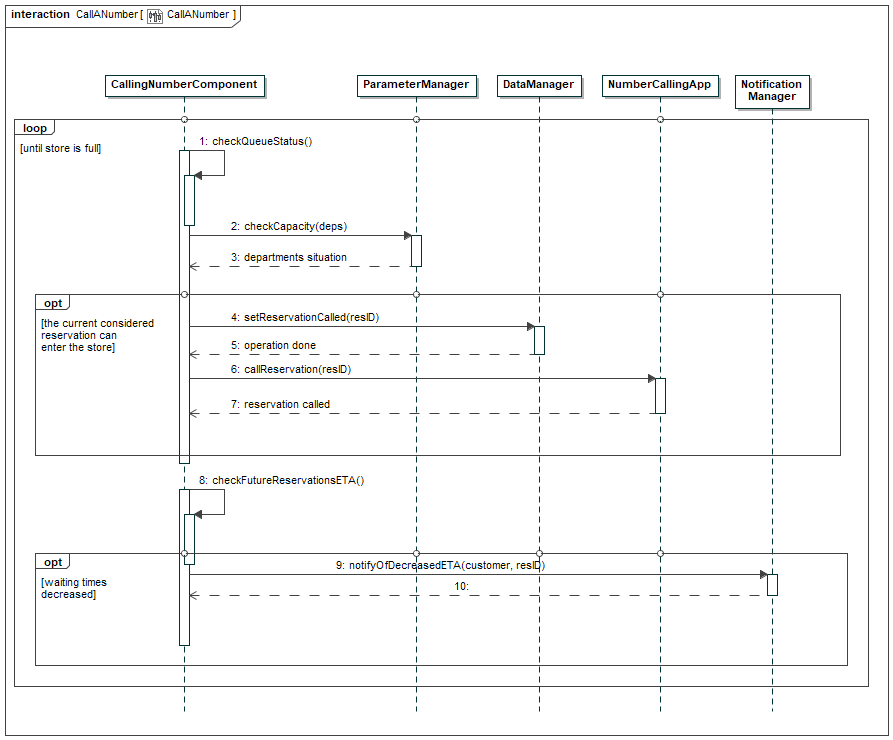
\includegraphics[scale=0.5]{Sequence Diagrams/sd__CallANumber__CallANumber.png}
		\end{adjustwidth}
		\caption{\emph{Calling Number Sequence Diagram}}
	\end{figure}	

	\bigskip
	
	The last process to be analysed is the notification when a customer should depart to get in time, and not too late to the store. As described before, this operation is entirely handled by the MobileApp: if this is processed by the server, it would be necessary to continuously request to the client the \emph{GPS} Position, forward it to Map Service to calculate the travel time, and if necessary send to the customer a notification. This may overload the server of useless traffic, since this operation can be handled by the MobileApp, directly accessing to the map external service and the \emph{GPS Module} of the mobile device running it.
	\begin{figure}[H]
		\begin{adjustwidth} {-1.8cm}{}
			\centering
			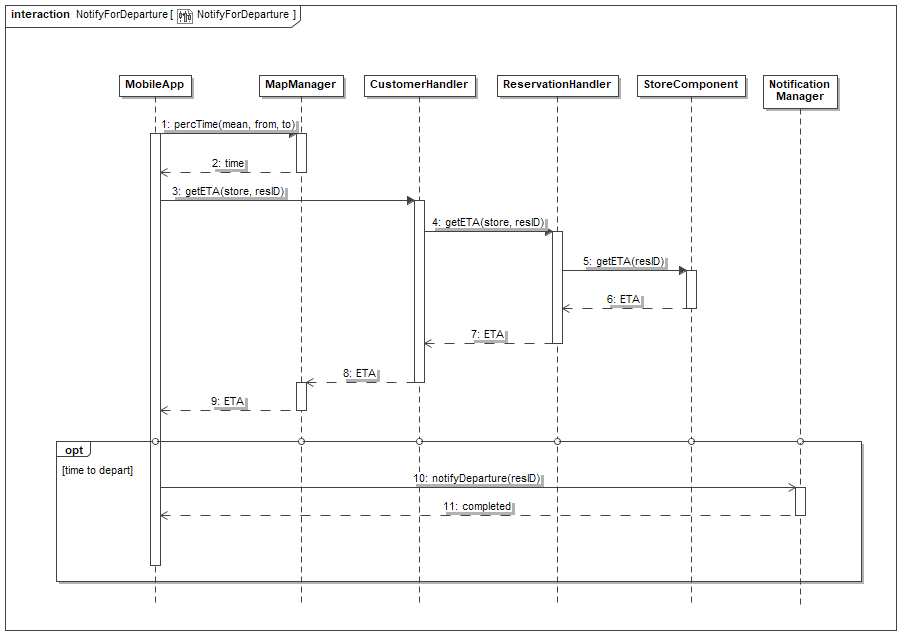
\includegraphics[scale=0.5]{Sequence Diagrams/sd__NotifyForDeparture__NotifyForDeparture.png}
		\end{adjustwidth}
		\caption{\emph{Calling Number Sequence Diagram}}
	\end{figure}

	The process is quite simple: the MobileApp requests to the MapManager the travel time from the current place, to the considered store, and by the mean of transport selected by the customer. Than, the \emph{ETA} for the call of the reservation is asked to the \emph{CLup} Server trough the ReservationHandler, that will forward the request to the correct StoreComponent. Finally, when all the data are available, the MobileApp processes them to infer if it's necessary to send an "internal" notification, in order to alert customer it's time to depart. If so, the NotificationManager is invoked, with a request for a \emph{Departure Notification}.
	\subsection{Component Interfaces}
	\begin{figure}
		\begin{adjustwidth} {0cm}{}
			\centering
			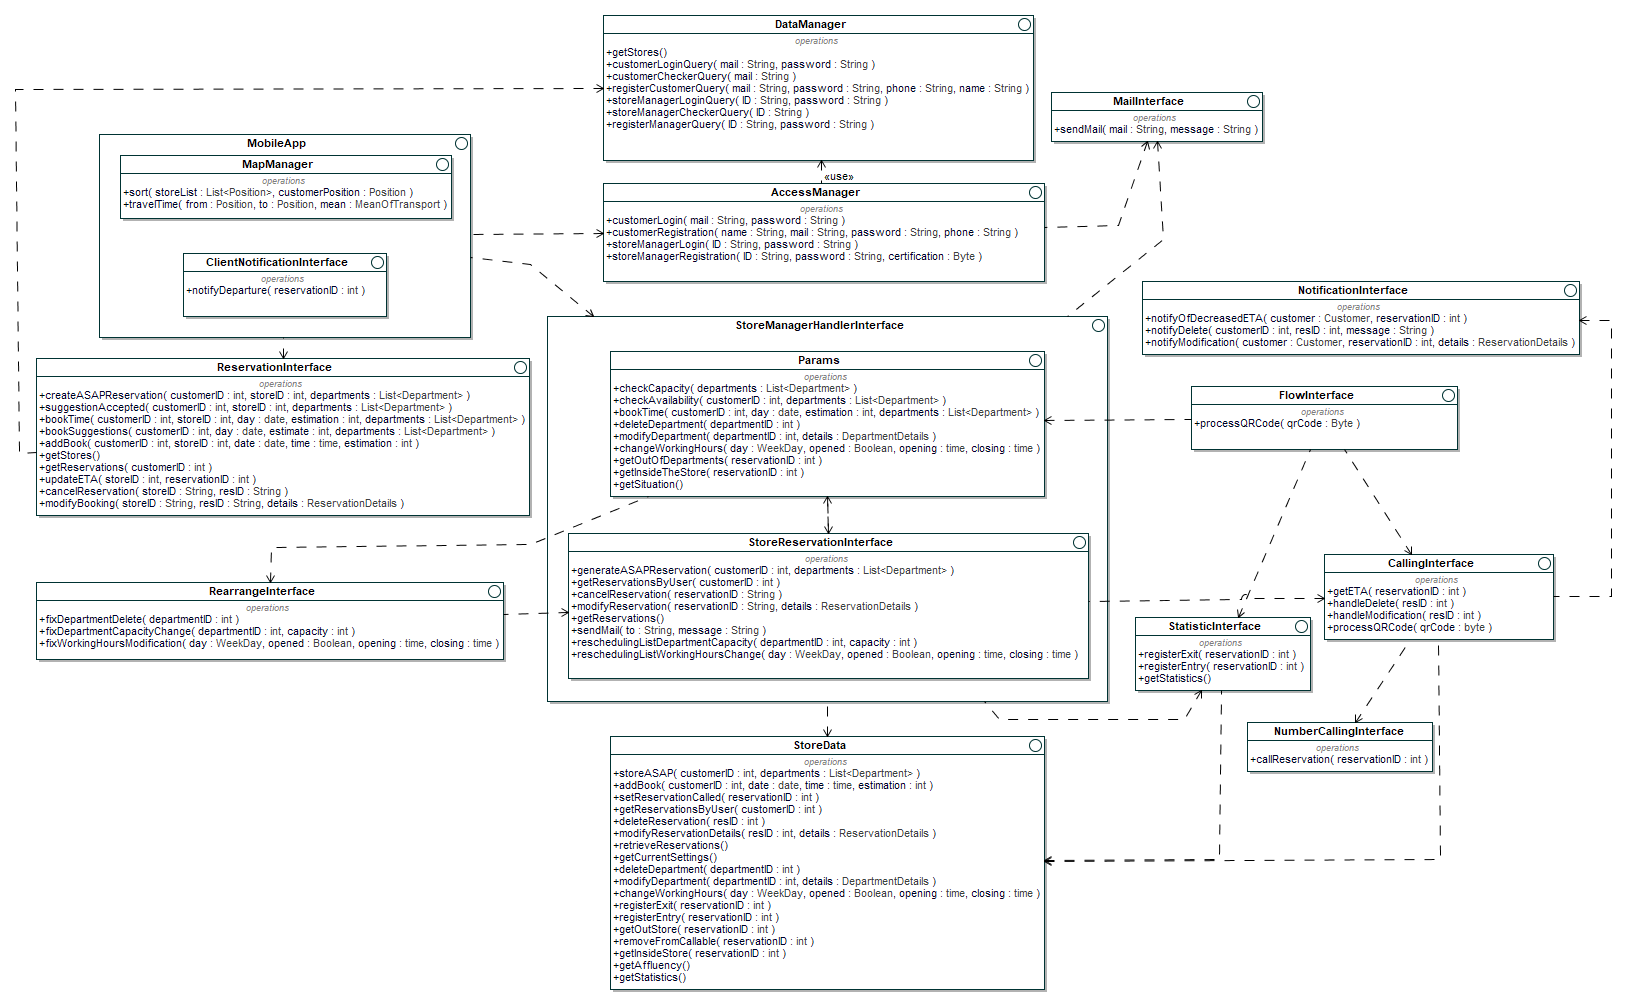
\includegraphics[scale=0.31, angle = 90]{Interface Diagram/class__InterfaceDiagram.png}
		\end{adjustwidth}
		\caption{\emph{Component Interfaces Diagram}}
	\end{figure}
	The previous diagram represents the interfaces of the most important and critic components of witch \emph{CLup} is composed. All of these interfaces contains the methods used in the previously described \emph{Sequence Diagrams}, and in such a way shows how the methods used by a component uses other parts of the system to complete its tasks. Not all the interfaces are described here, such as the one related to \emph{CustomerHandler}, since it is an adapter between \emph{presentation Tier} and \emph{Business Tier}, only going to repeat methods already reported.\\
	As \emph{Sequence Diagrams} are simplified, here the methods type and parameters are totally fictitious, and used only to gave an idea of the content transmitted from a component to another.
	\begin{itemize}
		\item {\bfseries StoreData}: it's exposed by the {\bfseries DataManager} of each {\bfseries StoreComponent}, and it's used by all the other component that needs to access to \emph{DBMS} to retrieve data, or to permanently modified informations related to the associated Store.
		\item {\bfseries StoreManagerHandlerInterface}: represents all the functionalities that a \emph{Store Manager} can access to using the \emph{MobileApp}. Since the main things that a manager can do is to manage reservations and settings of the store, this interface implements the two interfaces relative to the {\bfseries ParameterComponent} and to the {\bfseries ReservationComponent}. The first expose all the methods necessary to manage the settings of the store, and can also be used by other components, that need to access store preferences; the second is related to the management of store's reservation, and expose all the methods necessary to access and manage store's reservation.
		\item{\bfseries RearrangeInterface}: all the methods here described are related to the processes needed to put the store in a consistent state after some parameters (such as departments and working hours) are modified in a way that not all the requests can be satisfied.
		\item{\bfseries ReservationInterface}: implements all the methods necessary to allow a customer to do and to manage his own reservations. It acts like a forwarder of requests from the general server, where these methods are implemented, to the correct component of the store involved in the request. Moreover, there are functionalities designated to query all the stores in order to give customers suggestions on reservations, both \emph{ASAP} and \emph{Booked}.
		\item{\bfseries AccessInterface}: all the operations needed to process login and registration features are contained in this interface, that can be directly accessed from the \emph{Mobile App}. It makes use of the {\bfseries DataManager} to check and store credentials on the \emph{DBMS}.
		\item{\bfseries Data Interface}: exposes the methods needed by the components of the general server to access data necessary to do the business tasks related to the system, such as checking and storing credentials in respectively login and registration process, and to store all the stores that are managed by the system.
		\item{\bfseries FlowInterface}: defines the methods used by \emph{QR Code Scanner App} to make requests at the system, precisely to invoke the analysis and processing of a scanned \emph{QR Code}, so that precise actions are made depending on the given code, and a feedback is sent to the local store.
		\item{\bfseries CallingInterface}: contains the methods necessary to communicate and make requests to the component devoted for gradually admit people inside the store. For example these methods allow to rearrange the queue if some reservation is modified, or to get the \emph{ETA} associated to a specific reservation.
		\item{\bfseries StatisticInterface}: this interface allow to communicate with the {\bfseries StatisticComponent} in order to get visits' statistics, to create and update visits' data.
		\item{\bfseries NumberCallingInterface}: specifies methods necessary to notify something using the {\bfseries NumberCallingApp} that some reservation have been called inside the store.
		\item{\bfseries NotificationInterface}, {\bfseries MailInterface}, {\bfseries MapInterface} and {\bfseries ClientNotificationInterface}: the interfaces implemented by the adapters for using the respectively associated service.
		
		
		
	\end{itemize}
	\subsection{Selected Architectural Styles and Patterns}
	\subsubsection{System Architecture}
	As briefly introduced before, since \emph{CLup} is a service usable by a great amount of people, and the operations made trough the systems must be considered in each function everyone can access, the architectural style best fitting for the described service is the {\bfseries client-server} one. In fact, there are clients that make requests to a server, that processes them and reply to clients with the response of each computation.\\
	In implementing the {\bfseries client-server} architecture many alternatives have been analysed, but at the end the more suitable for \emph{CLup} scope is a {\bfseries three tier architecture}, that, as previously said and described, logically separates the {\bfseries presentation}, {\bfseries business} and {\bfseries data} tier.\\
	A particular description must be done about the particular {\bfseries business} and {\bfseries data} tier here implemented. In fact, in the system there isn't a unique principal business component, and/or a unique data tier. Since each store is independent from the other, and should access only to data of their competence, the business tier is divided so that each store has his own business logic. This helps in various situations, such as greater flexibility in accepting managers requests to implement a certain business logic, maybe different from the one of some other store; in case of dysfunctionality, only the broken store won't work, while the components of the others will work, and it's easier to isolate the broken one and repairing it without touching anything else; each store's {\bfseries business tier} has an associated and unique {\bfseries data tier} to access: this allows to separate each store's data, in order to make data consultation faster and more secure, since each store can access only to the associated \emph{DBMS}.\\
	\begin{figure}
		\begin{adjustwidth} {0cm}{}
			\centering
			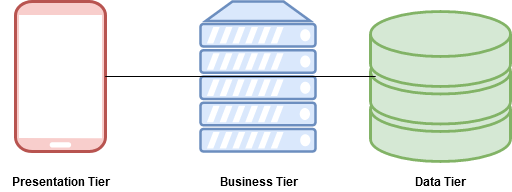
\includegraphics[scale=0.5]{ThreeTier.png}
		\end{adjustwidth}
		\caption{\emph{The Three Tier Architecture}}
	\end{figure}
	An advantage of this is that each client that makes operation on a single store, can connect directly to the correct {\bfseries business tier}. Regarding customers, instead, they connect to a dedicated {\bfseries business tier} with its own {\bfseries data tier}; it's scope it's to redirect requests from customers to a specific store, and to generate suggestions querying all the possible stores, which informations are stored in the general \emph{DBMS}.
	\subsubsection{Used Patterns}
	In this section will be described some of the \emph{design patterns} used in the development of \emph{CLup}.
	\begin{itemize}
		\item {\bfseries Pattern Adapter}: the adapter pattern have been used in multiple part \emph{CLup}. For example, each external service is accessed though an adapter that takes requests, and send them to the requires service. This help to easily implement multiple external service or to change them without a great effort. Moreover, also the {\bfseries CLup server} is an adapter, since takes in requests from the \emph{Mobile App} and redirects them to the correct {\bfseries StoreComponent}.
		\item{\bfseries Model View Controller}: this design pattern is used in each client developed for the system.
		\item{\bfseries Facade Pattern}: used to allow the {\bfseries StoreManagerHandler} to access more easily to multiple components trough the different interfaces they implement.
	\end{itemize}
	
\section{User Interface Design}
This section shows and describes accurately the mockups of the application, in order to explain how the main functionalities will be offered. The first subsection is dedicated to the illustration of the application flow, shown using two different \emph{UX diagram}, one for the customer and one for the store manager.
	\subsection{UX Diagrams}
	The following figures shows the application flow from the customer and the store manager point of view.
	
		\subsubsection{Customer Flow}
			\begin{figure}[H]
				\begin{adjustwidth} {0cm}{}
					\centering
					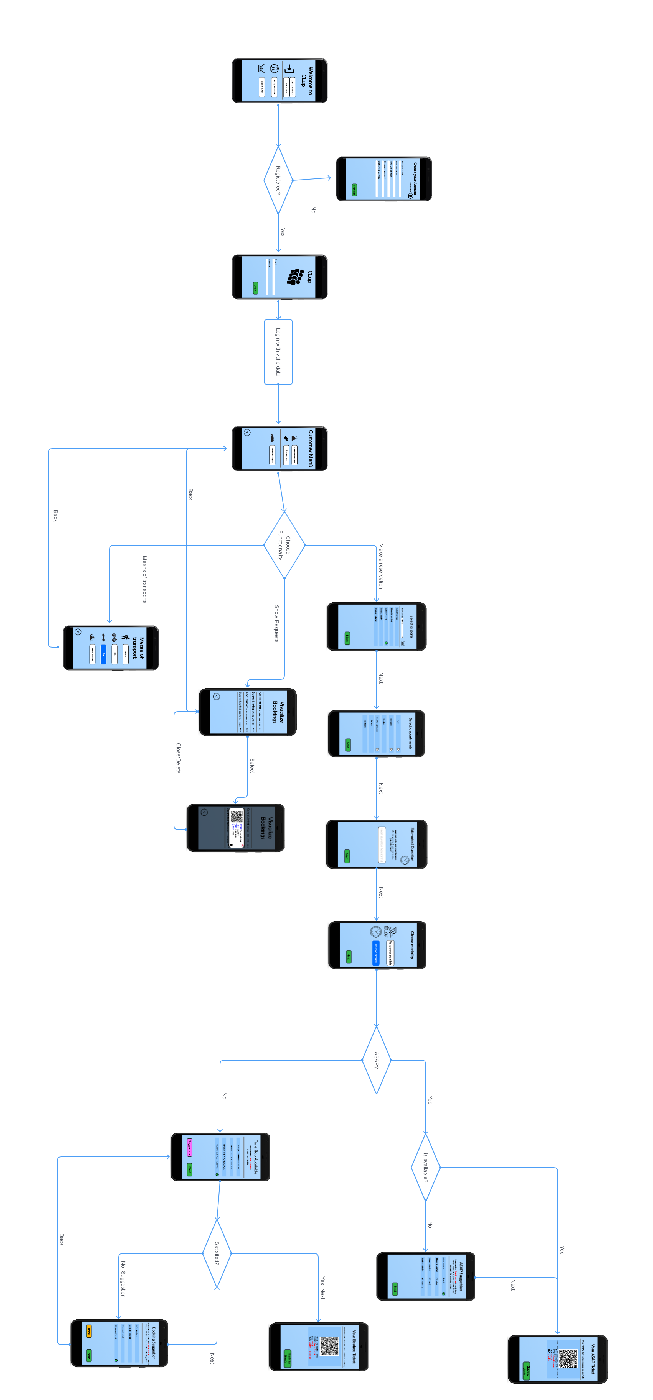
\includegraphics[scale=0.7, angle=180, trim= 0 0 0 0cm]{../Mockups/UXDiagrams/CustomerFlow.pdf}
				\end{adjustwidth}
				\caption{\emph{Customer Flow}}
			\end{figure}
		\subsubsection{Store Manager Flow}
			\begin{figure}[H]
				\begin{adjustwidth} {0cm}{}
				\centering
				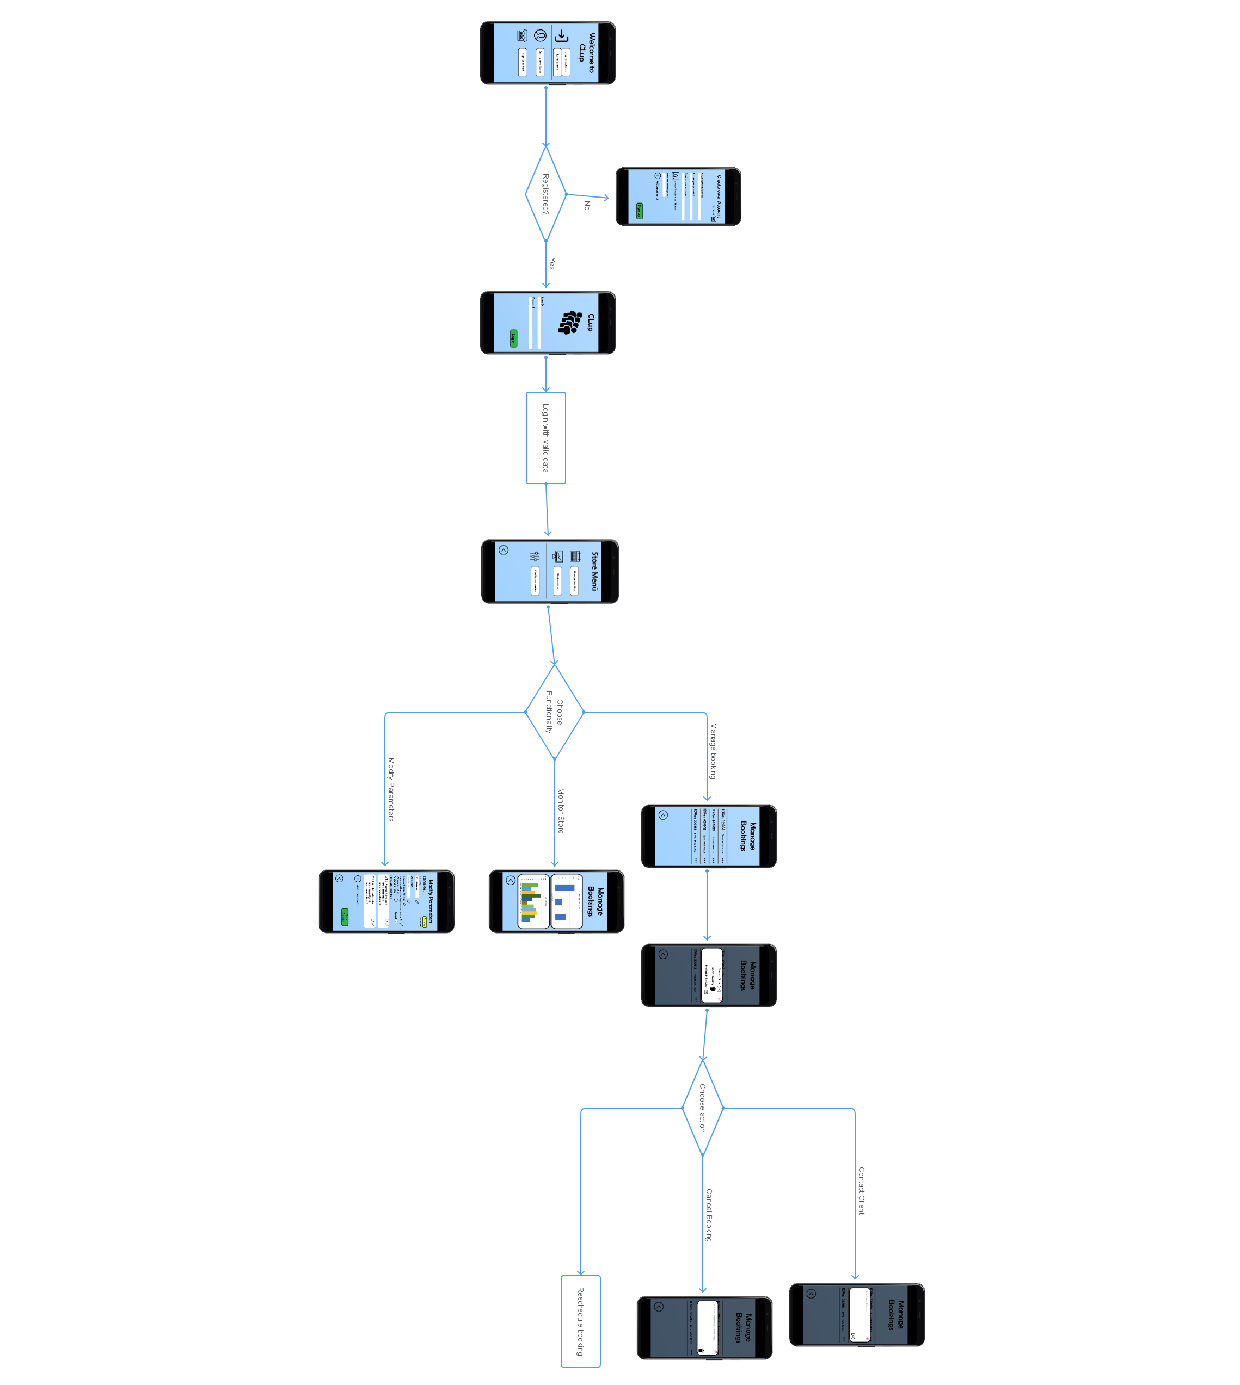
\includegraphics[scale=0.7, angle=180, trim= 0 0 0 0cm]{../Mockups/UXDiagrams/StoreManagerFlow.pdf}
				\end{adjustwidth}
			\caption{\emph{Store Manager Flow}}
			\end{figure}

	\subsection{User Mobile App}
	In this paragraph are shown mockups that are used to define which interfaces are present within the application. All interfaces are shown and accompanied by a description explaining their functionality. The {\bfseries Mobile App} version is truly intuitive and can be used without problems by everyone, customers or store managers. The application is flanked by totems placed at the entrance of each store, in case someone does not have the application or does not have a telephone and they only have one type of reservation, that is the \emph{ASAP} one, in the shop they belong to.
	
		\subsubsection{Home Page}
		In this section is shown the initial page that a user finds when opening the app. From this section the user can make a new registration, if is not registered yet, or can sign-in in order to use the functionalities that the app offers.
		\bigskip
		\bigskip
		\begin{figure}[!h]
			\begin{adjustwidth} {0cm}{}
				\centering
				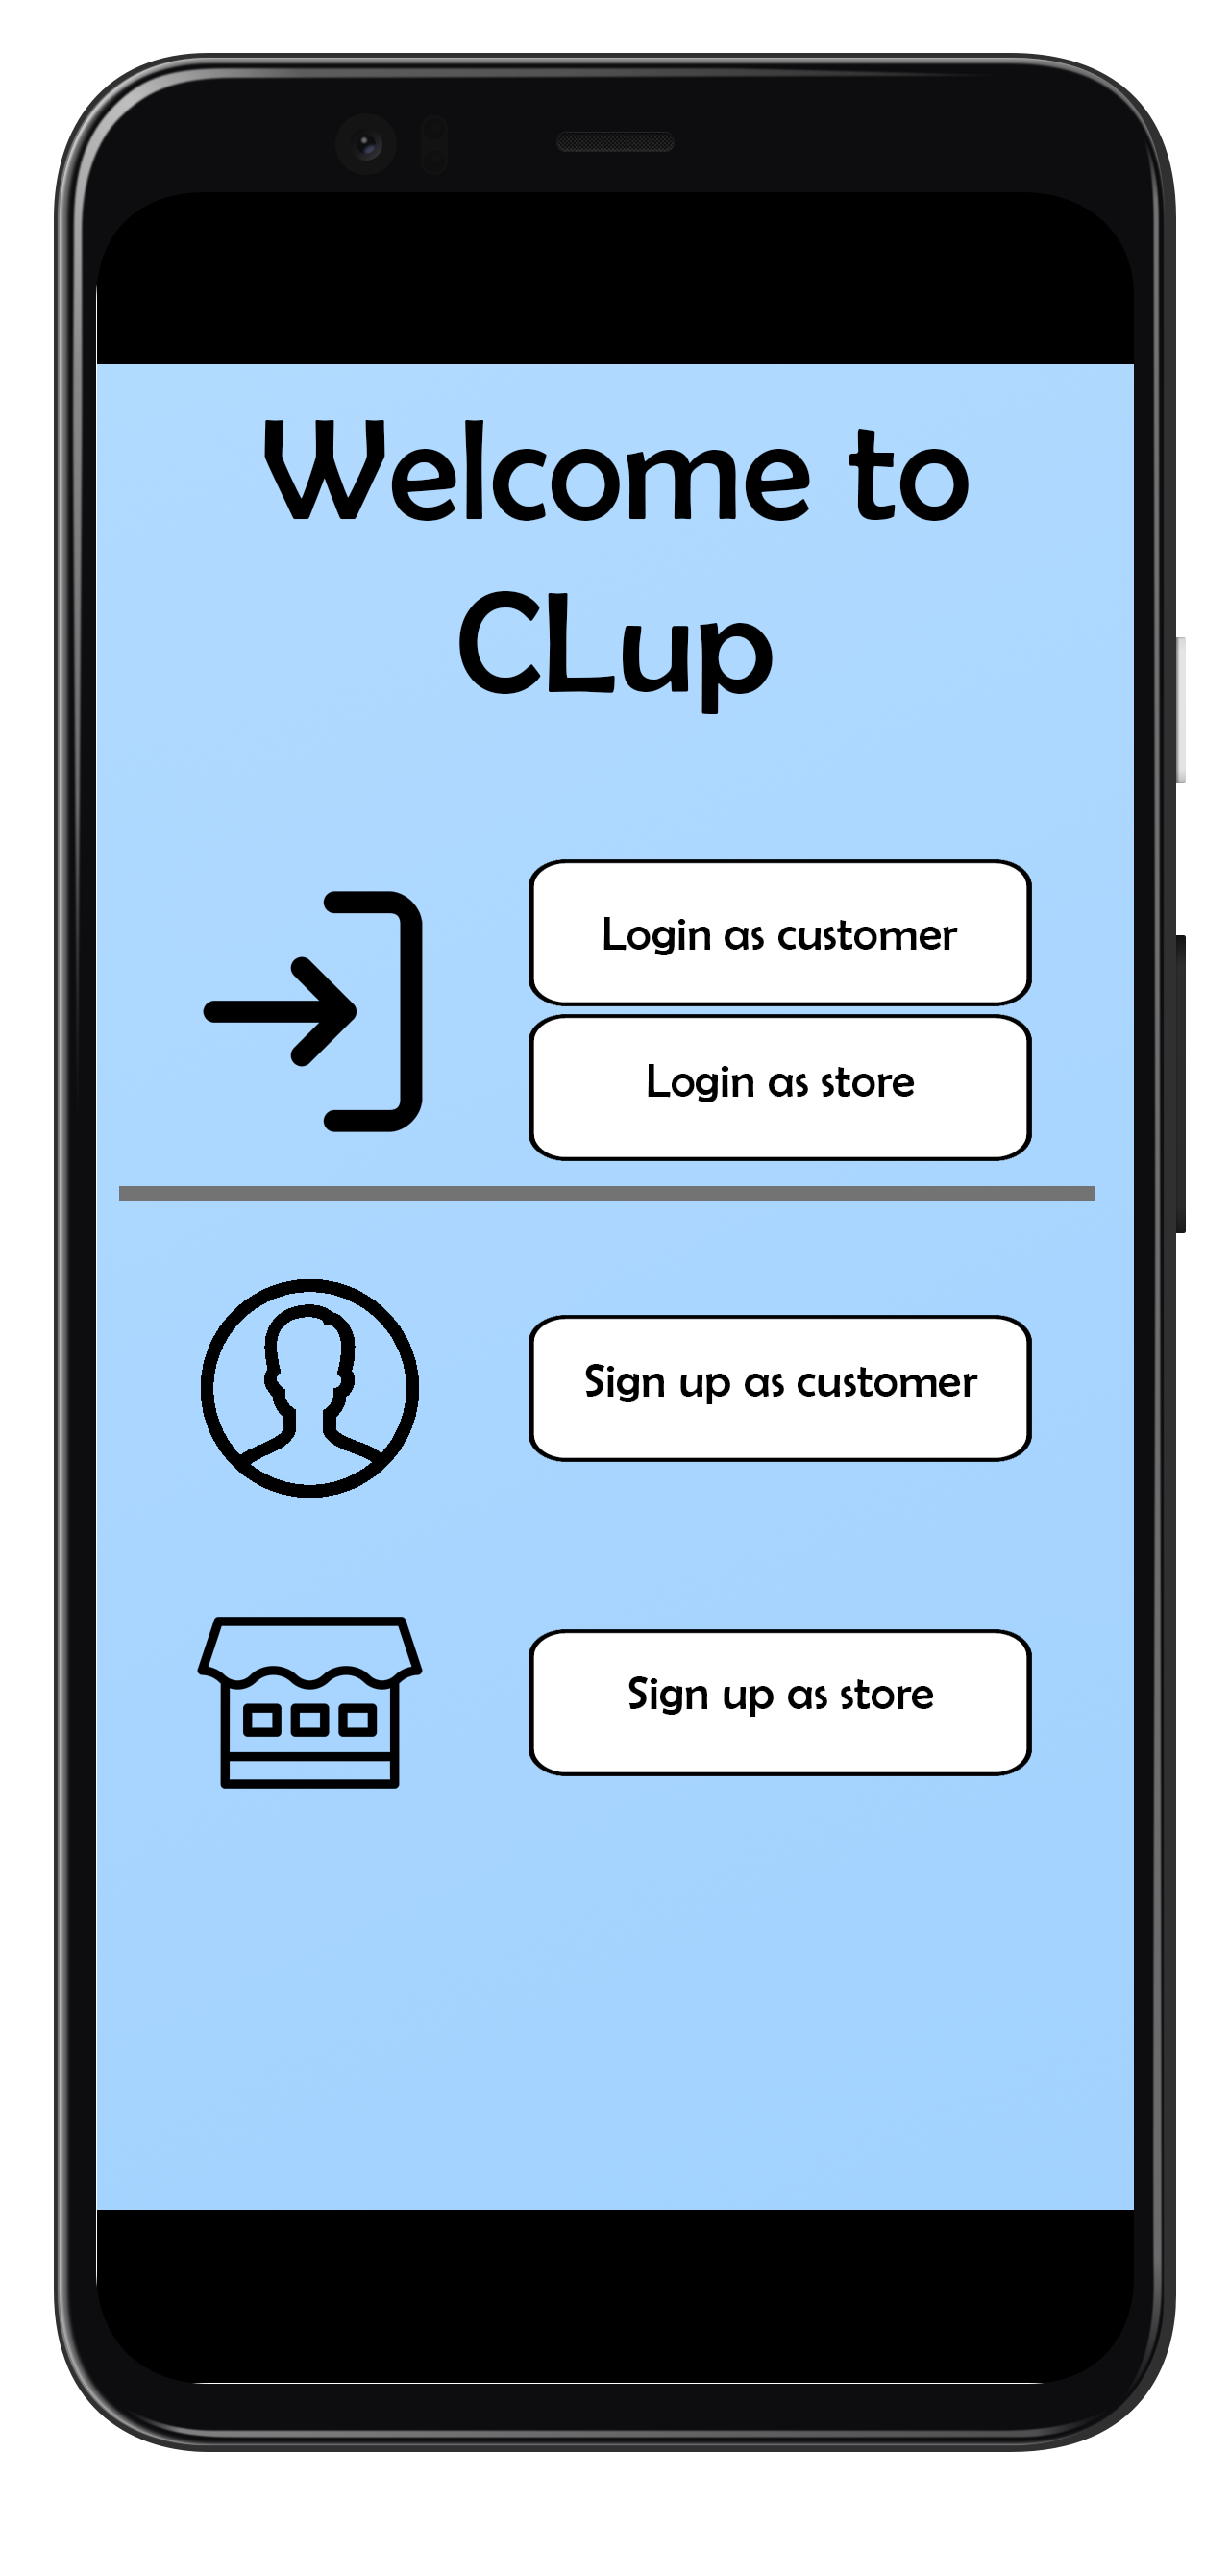
\includegraphics[scale=0.15]{../Mockups/InitialPage.png}\\
			\end{adjustwidth}
			\caption{\emph{Home page}}
		\end{figure}
		
		\newpage
		\subsubsection{Registration}
		In this section are shown the mockups about the registration of an user. In fact an user can make a registration as a customer or as a store, based on the role it must have inside the app.
		\begin{itemize}
			\item If an user decides to create a customer account have to enter some parameter (email, name, password) in order to complete the registration.
			\item If an user decided to create a store manager account have to enter a valid store certification and a password.
		\end{itemize}
		\bigskip
		\bigskip
		\begin{figure}[!h]
			\centering
			\begin{minipage}[!h]{0.4\textwidth}
				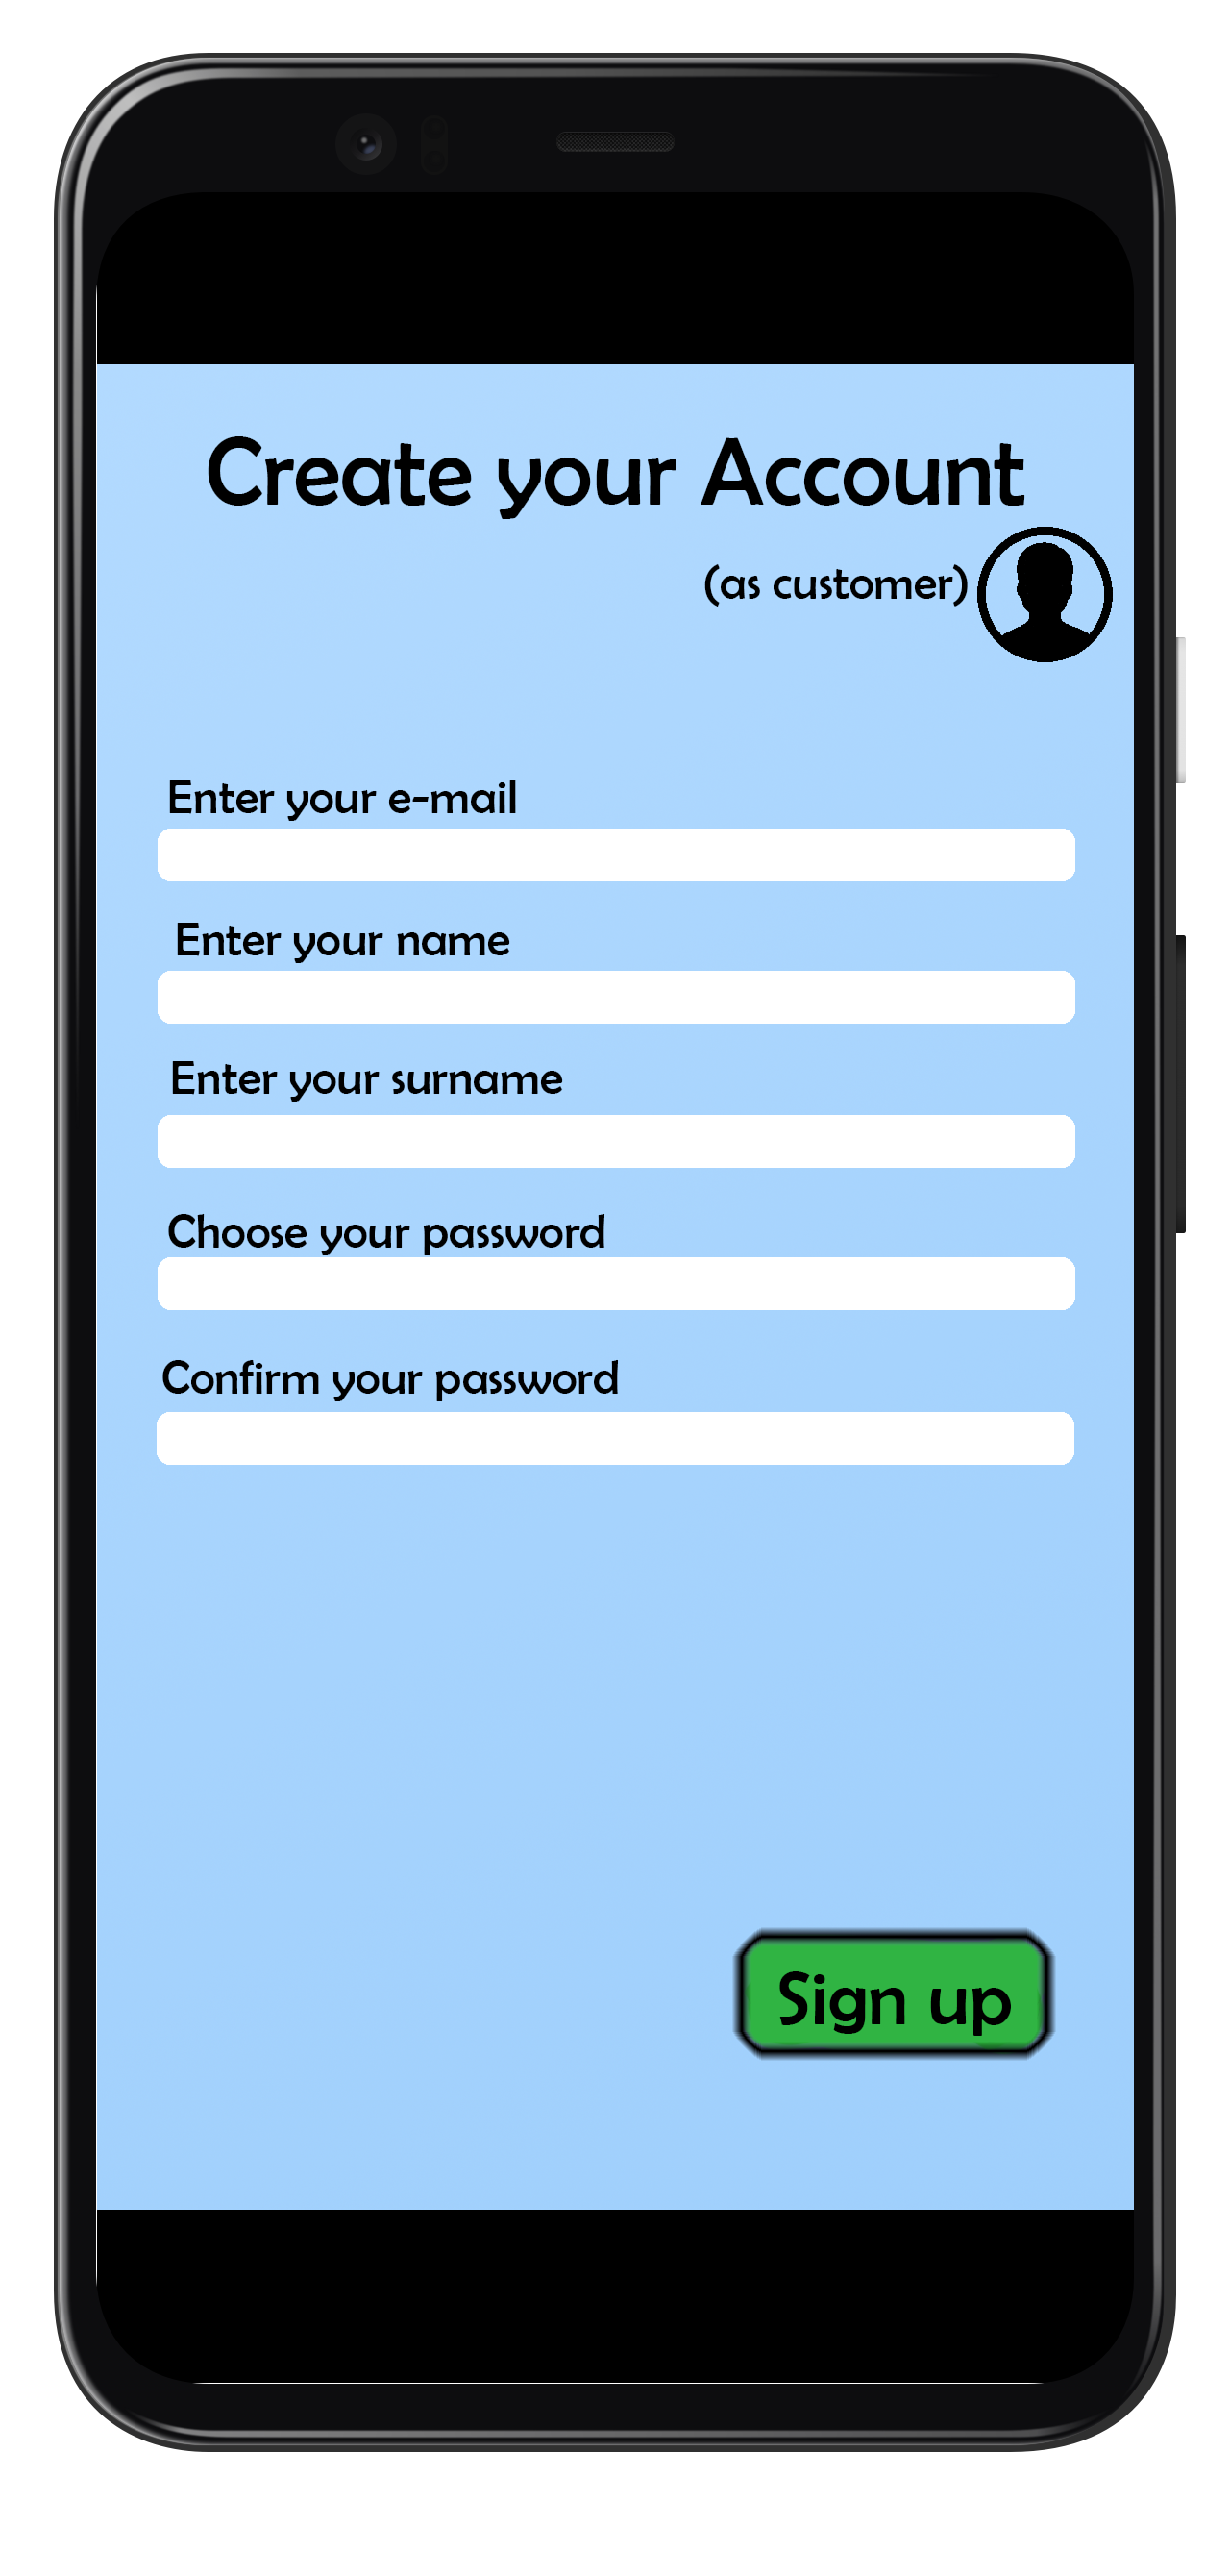
\includegraphics[width=\textwidth]{../Mockups/SignUpCustomer.png}
				\caption{\emph{Sign up as customer}}
			\end{minipage}
			\hfill
			\begin{minipage}[!h]{0.4\textwidth}
				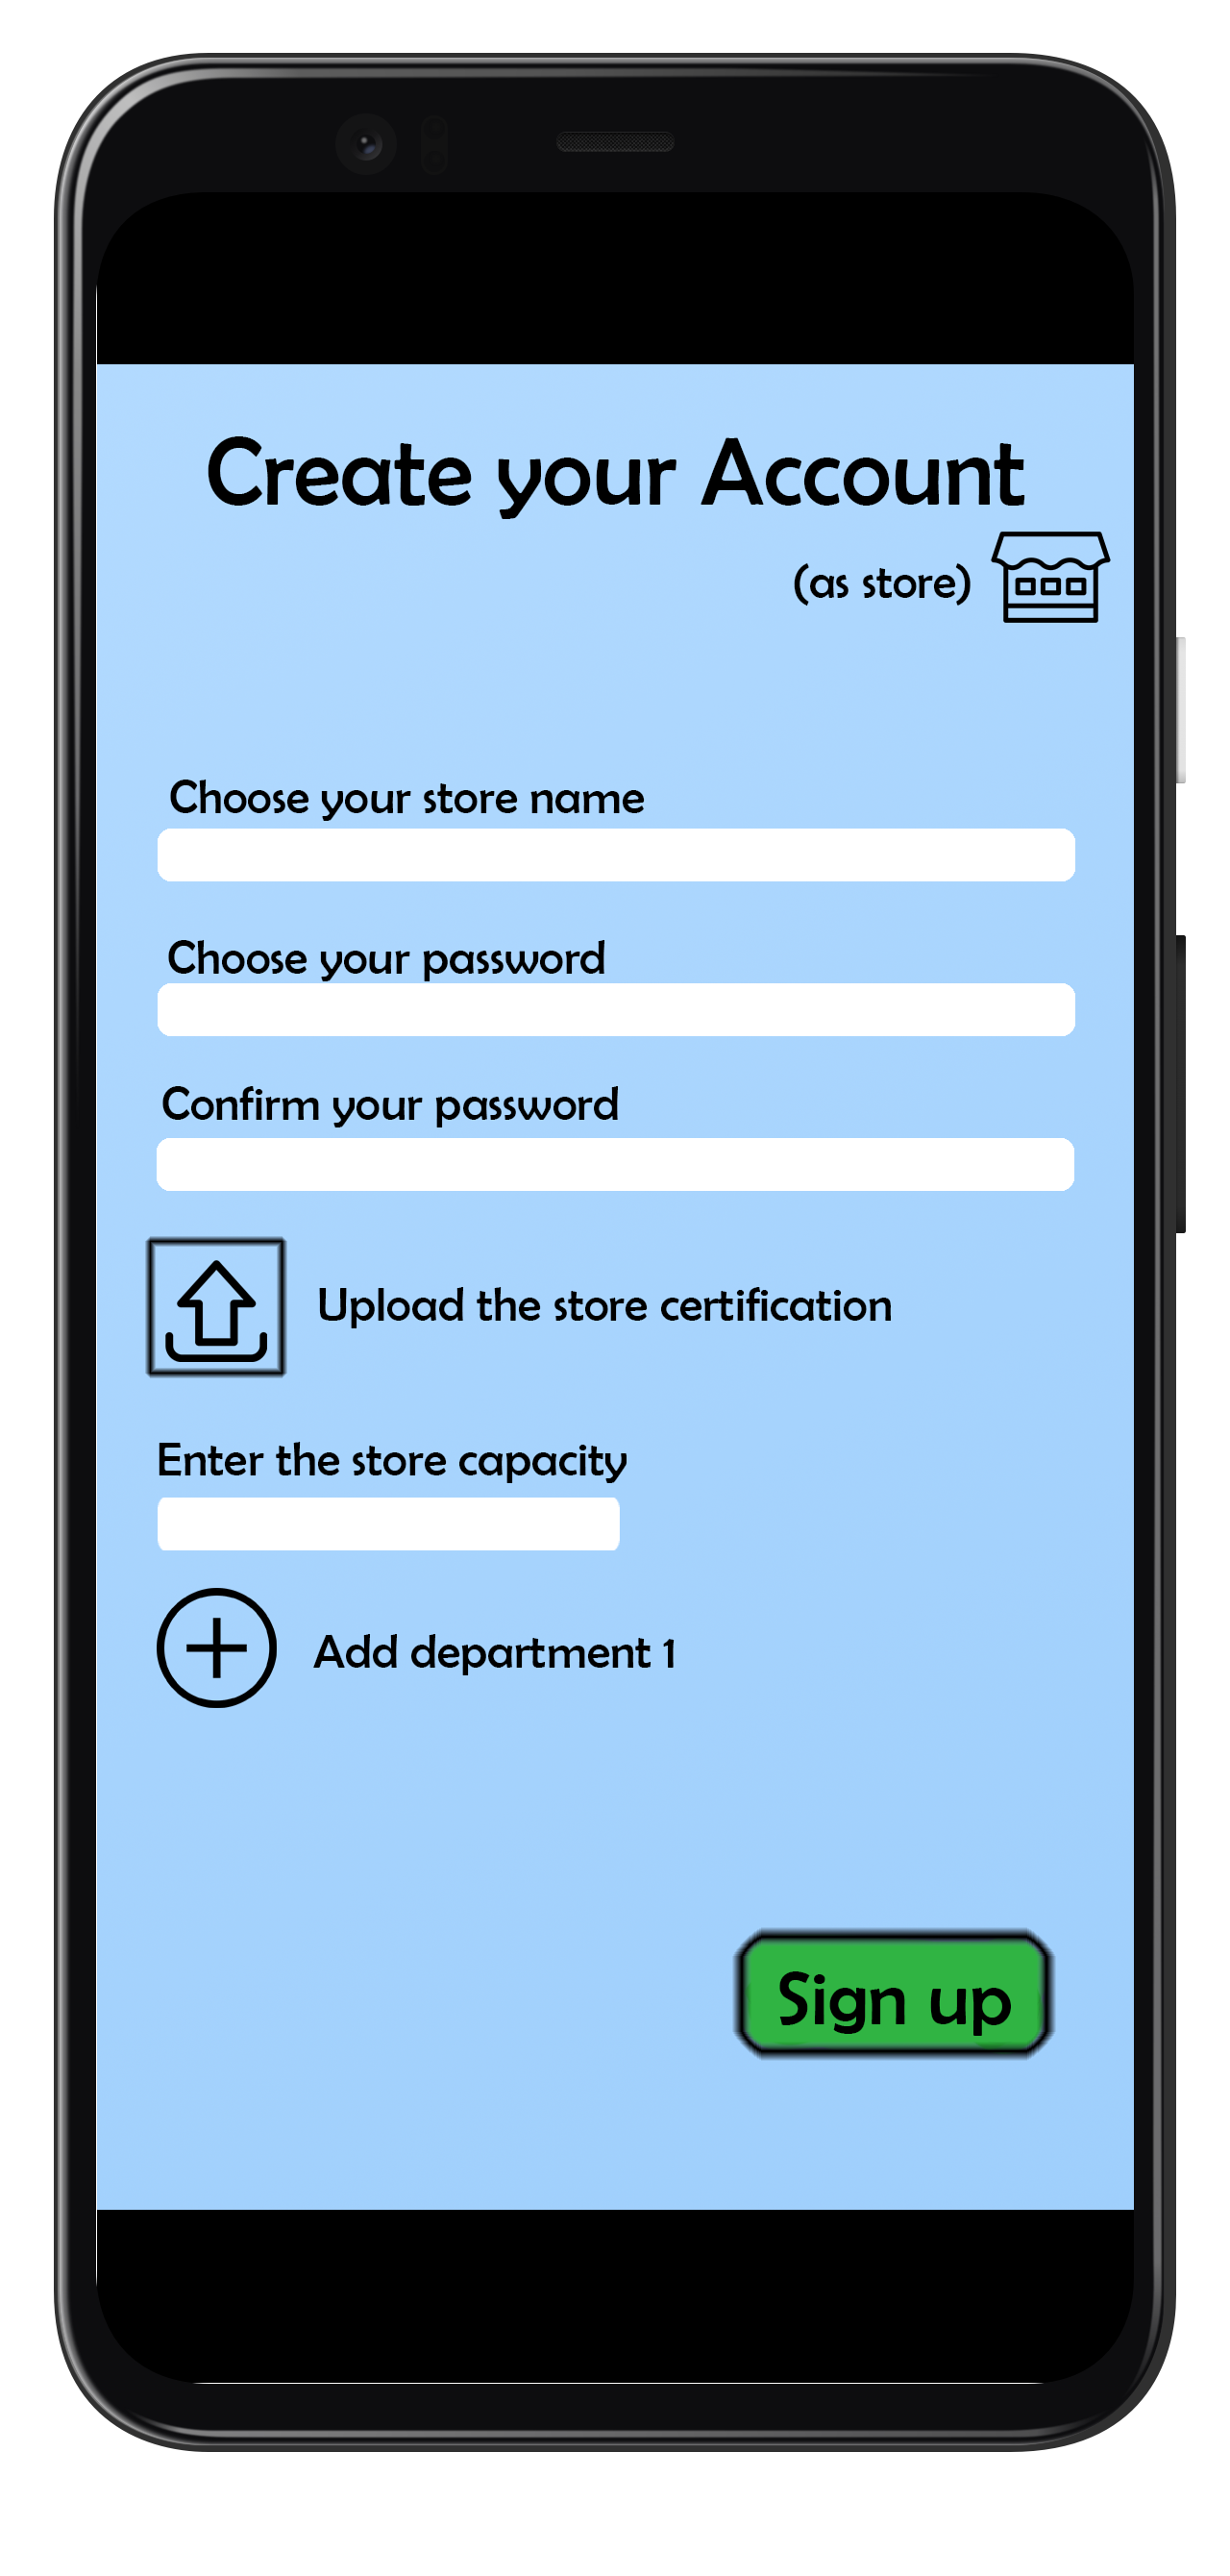
\includegraphics[width=\textwidth]{../Mockups/SignUpStore.png}
				\caption{\emph{Sign up as store manager}}
			\end{minipage}
		\end{figure}
		
		\newpage
		
		\subsubsection{Login}
		In this section are shown the mockups about the login of an user. In fact an user can perform two types of login based on the type of registration made at a previous time.
		\begin{itemize}
			\item If an user has registered as customer have to put email and password in the respective fields.
			\item If an user has registered as store manager have to put Store \emph{ID} and password in the respective fields.
		\end{itemize}
		\bigskip
		\bigskip
		\begin{figure}[!h]
			\centering
			\begin{minipage}[!h]{0.4\textwidth}
				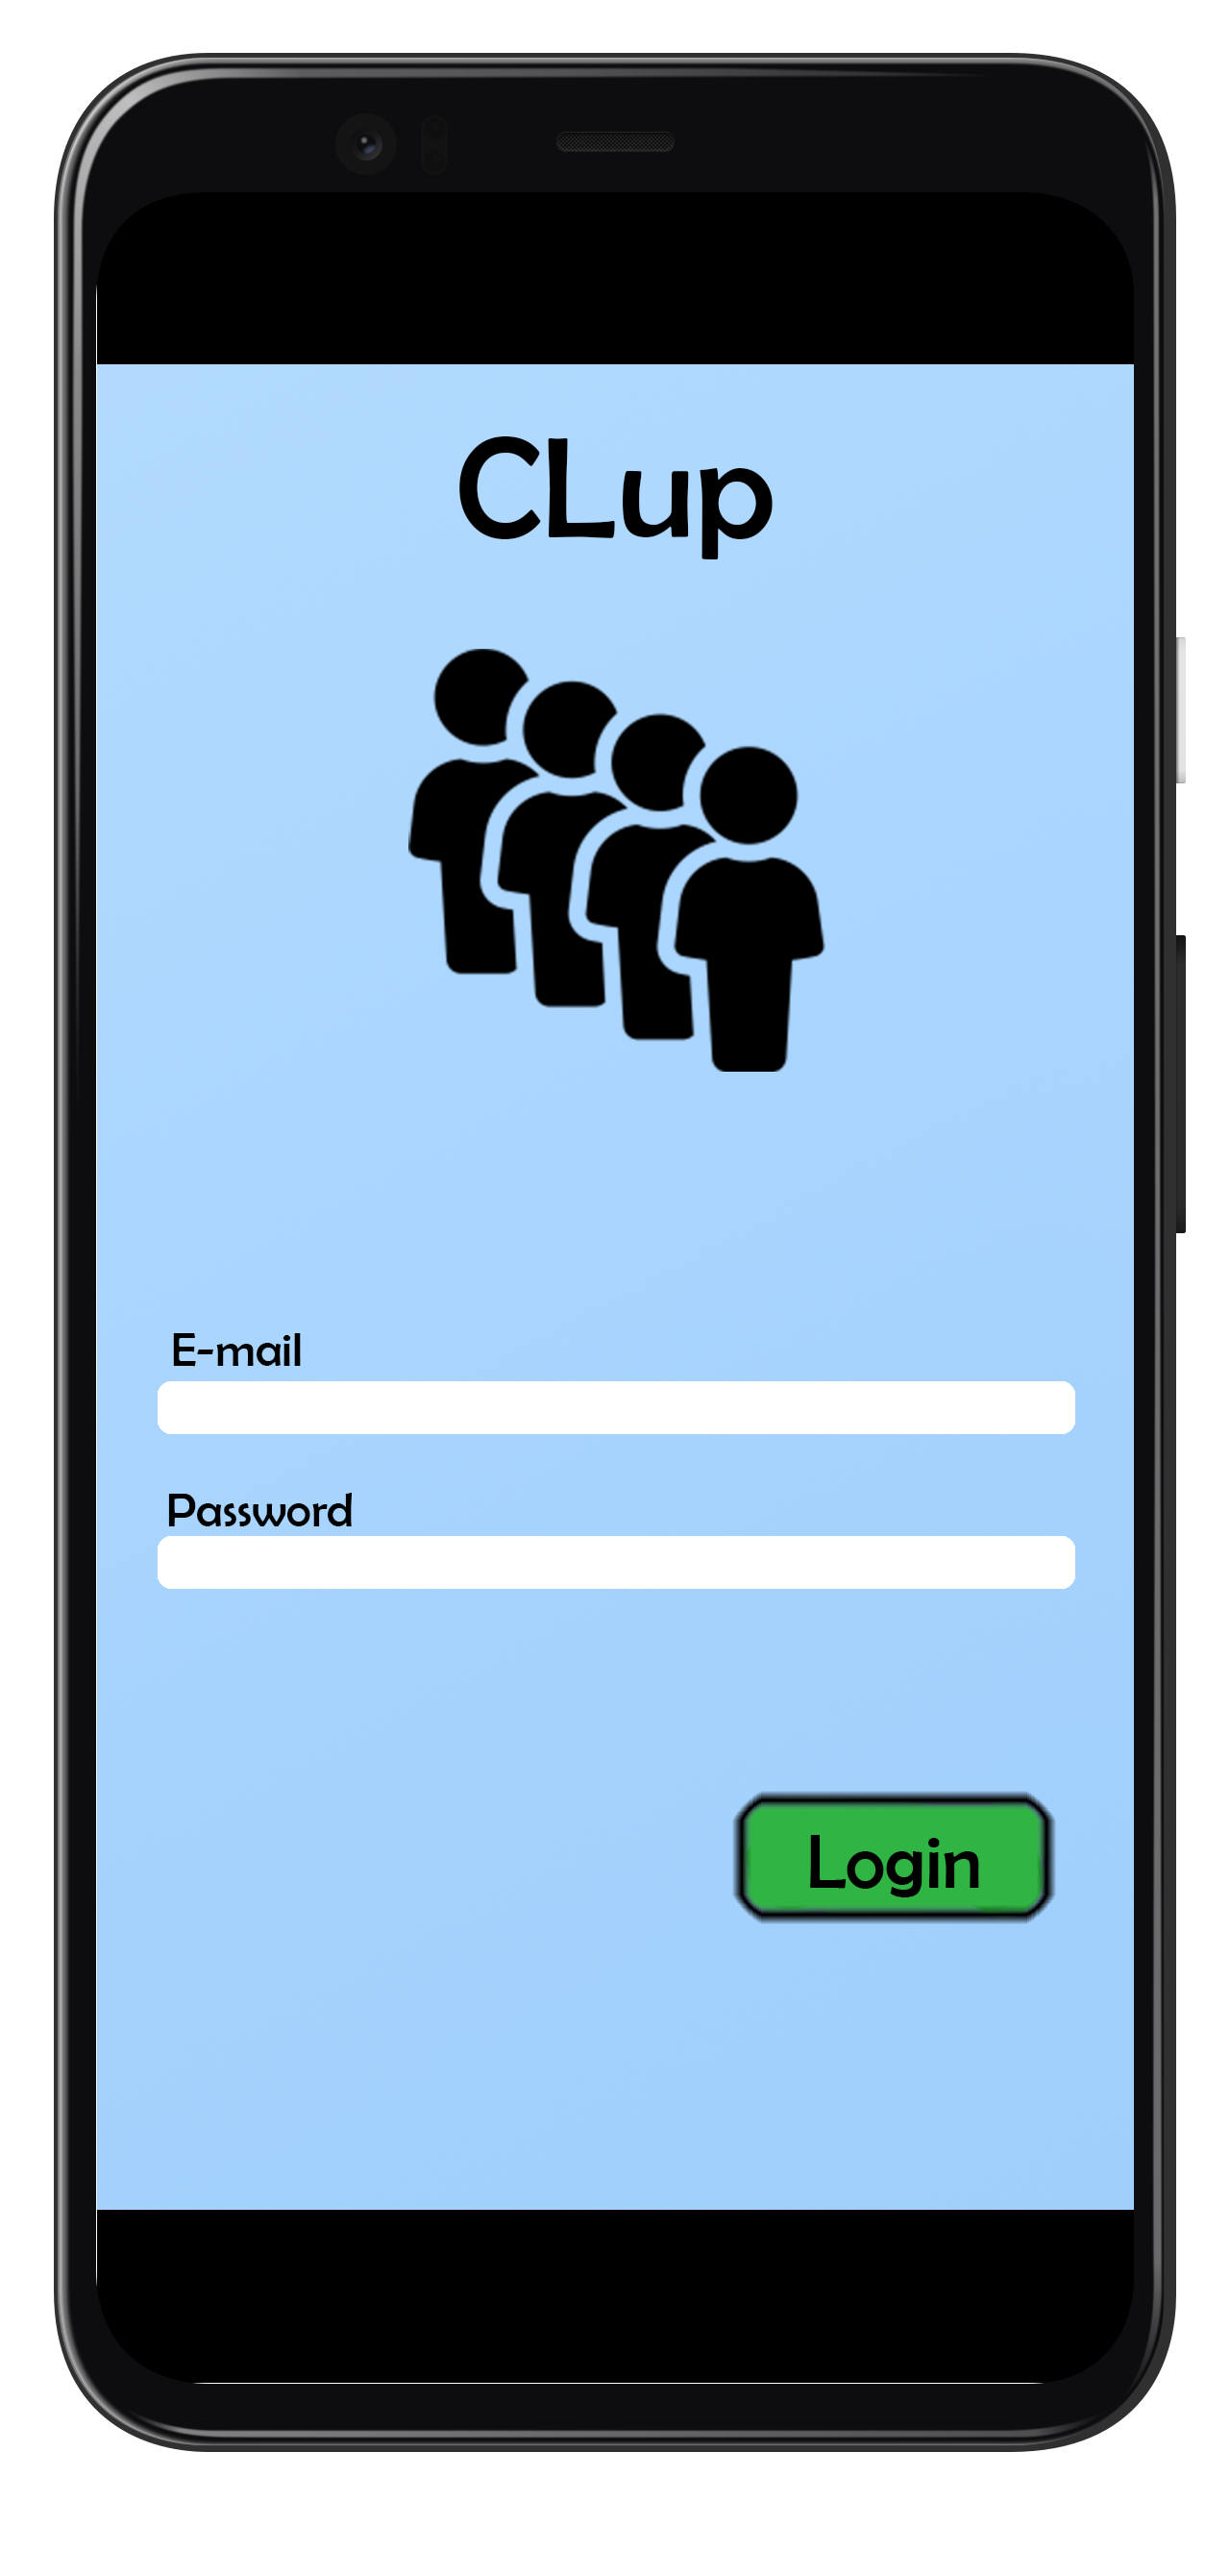
\includegraphics[width=\textwidth]{../Mockups/LoginCustomer.png}
				\caption{\emph{Login as customer}}
			\end{minipage}
			\hfill
			\begin{minipage}[!h]{0.4\textwidth}
				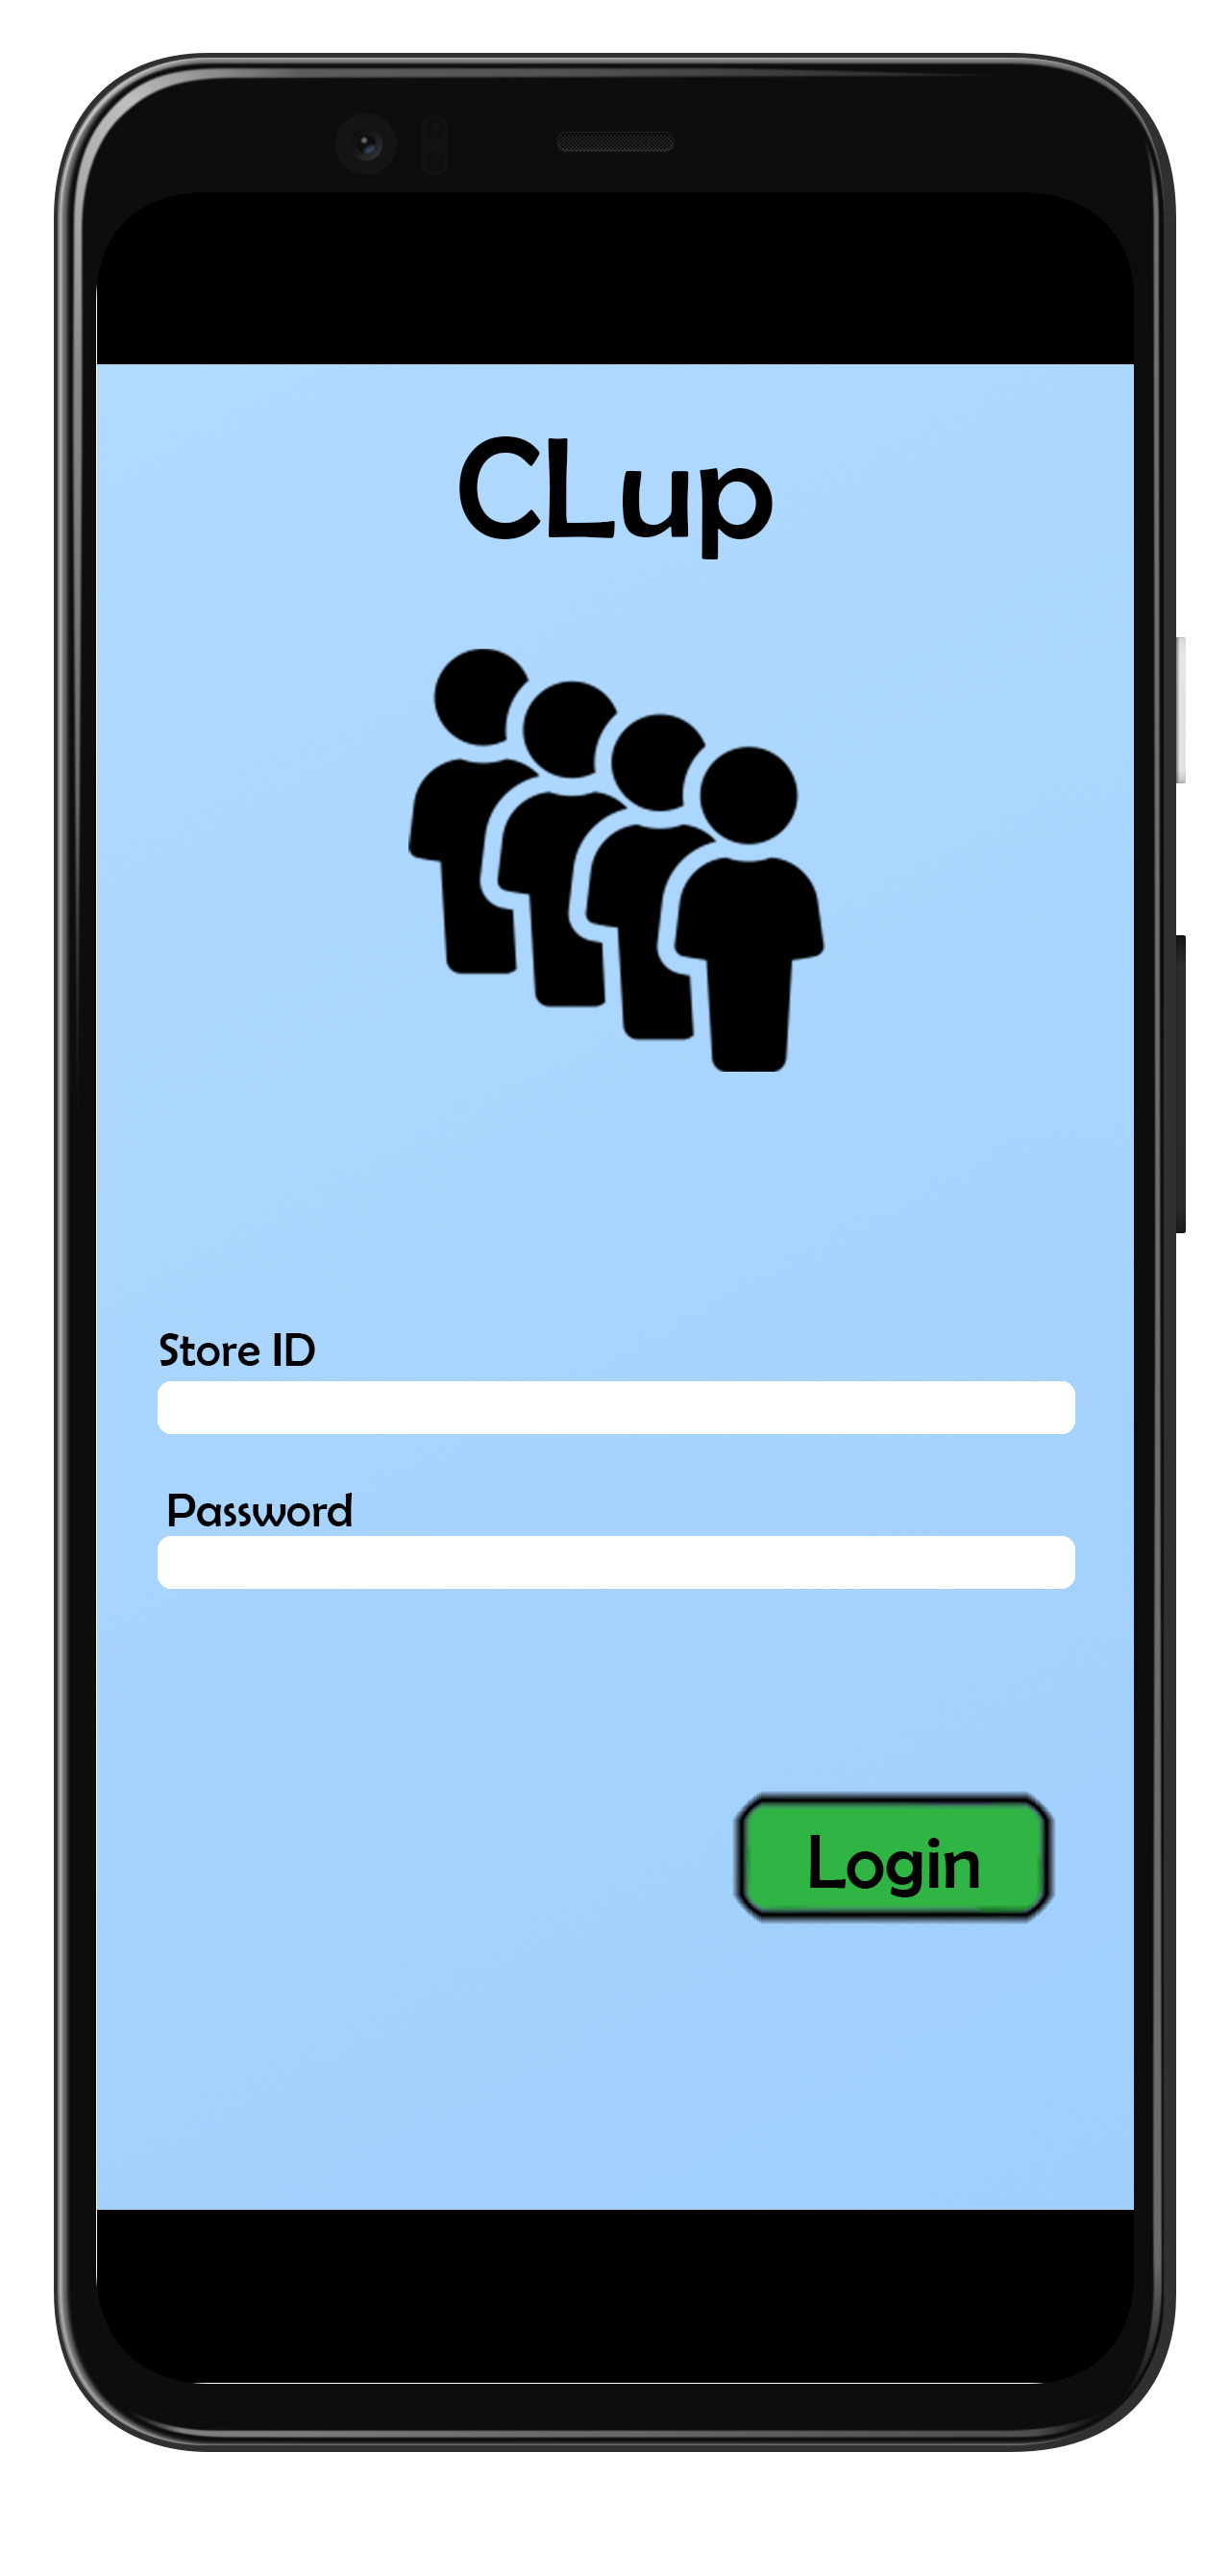
\includegraphics[width=\textwidth]{../Mockups/LoginStore.png}
				\caption{\emph{Login as a store}}
			\end{minipage}
		\end{figure}	
	
		\newpage
		
		\subsubsection{Menù}
		In this section are shown the mockups about main menù. After the login the users have a main menù that can be of two type, based on the type of the account: customer or store manager.
		\begin{itemize}
			\item In case of the customer, the menù allows to start a new reservation, show current requests and select the mean of transport.
			\item In case of the store manager, the menù allows to manage all reservations, see the store statistic and modify all store parameters.
		\end{itemize}
		\bigskip
		\bigskip
		\begin{figure}[!h]
			\centering
			\begin{minipage}[!h]{0.4\textwidth}
				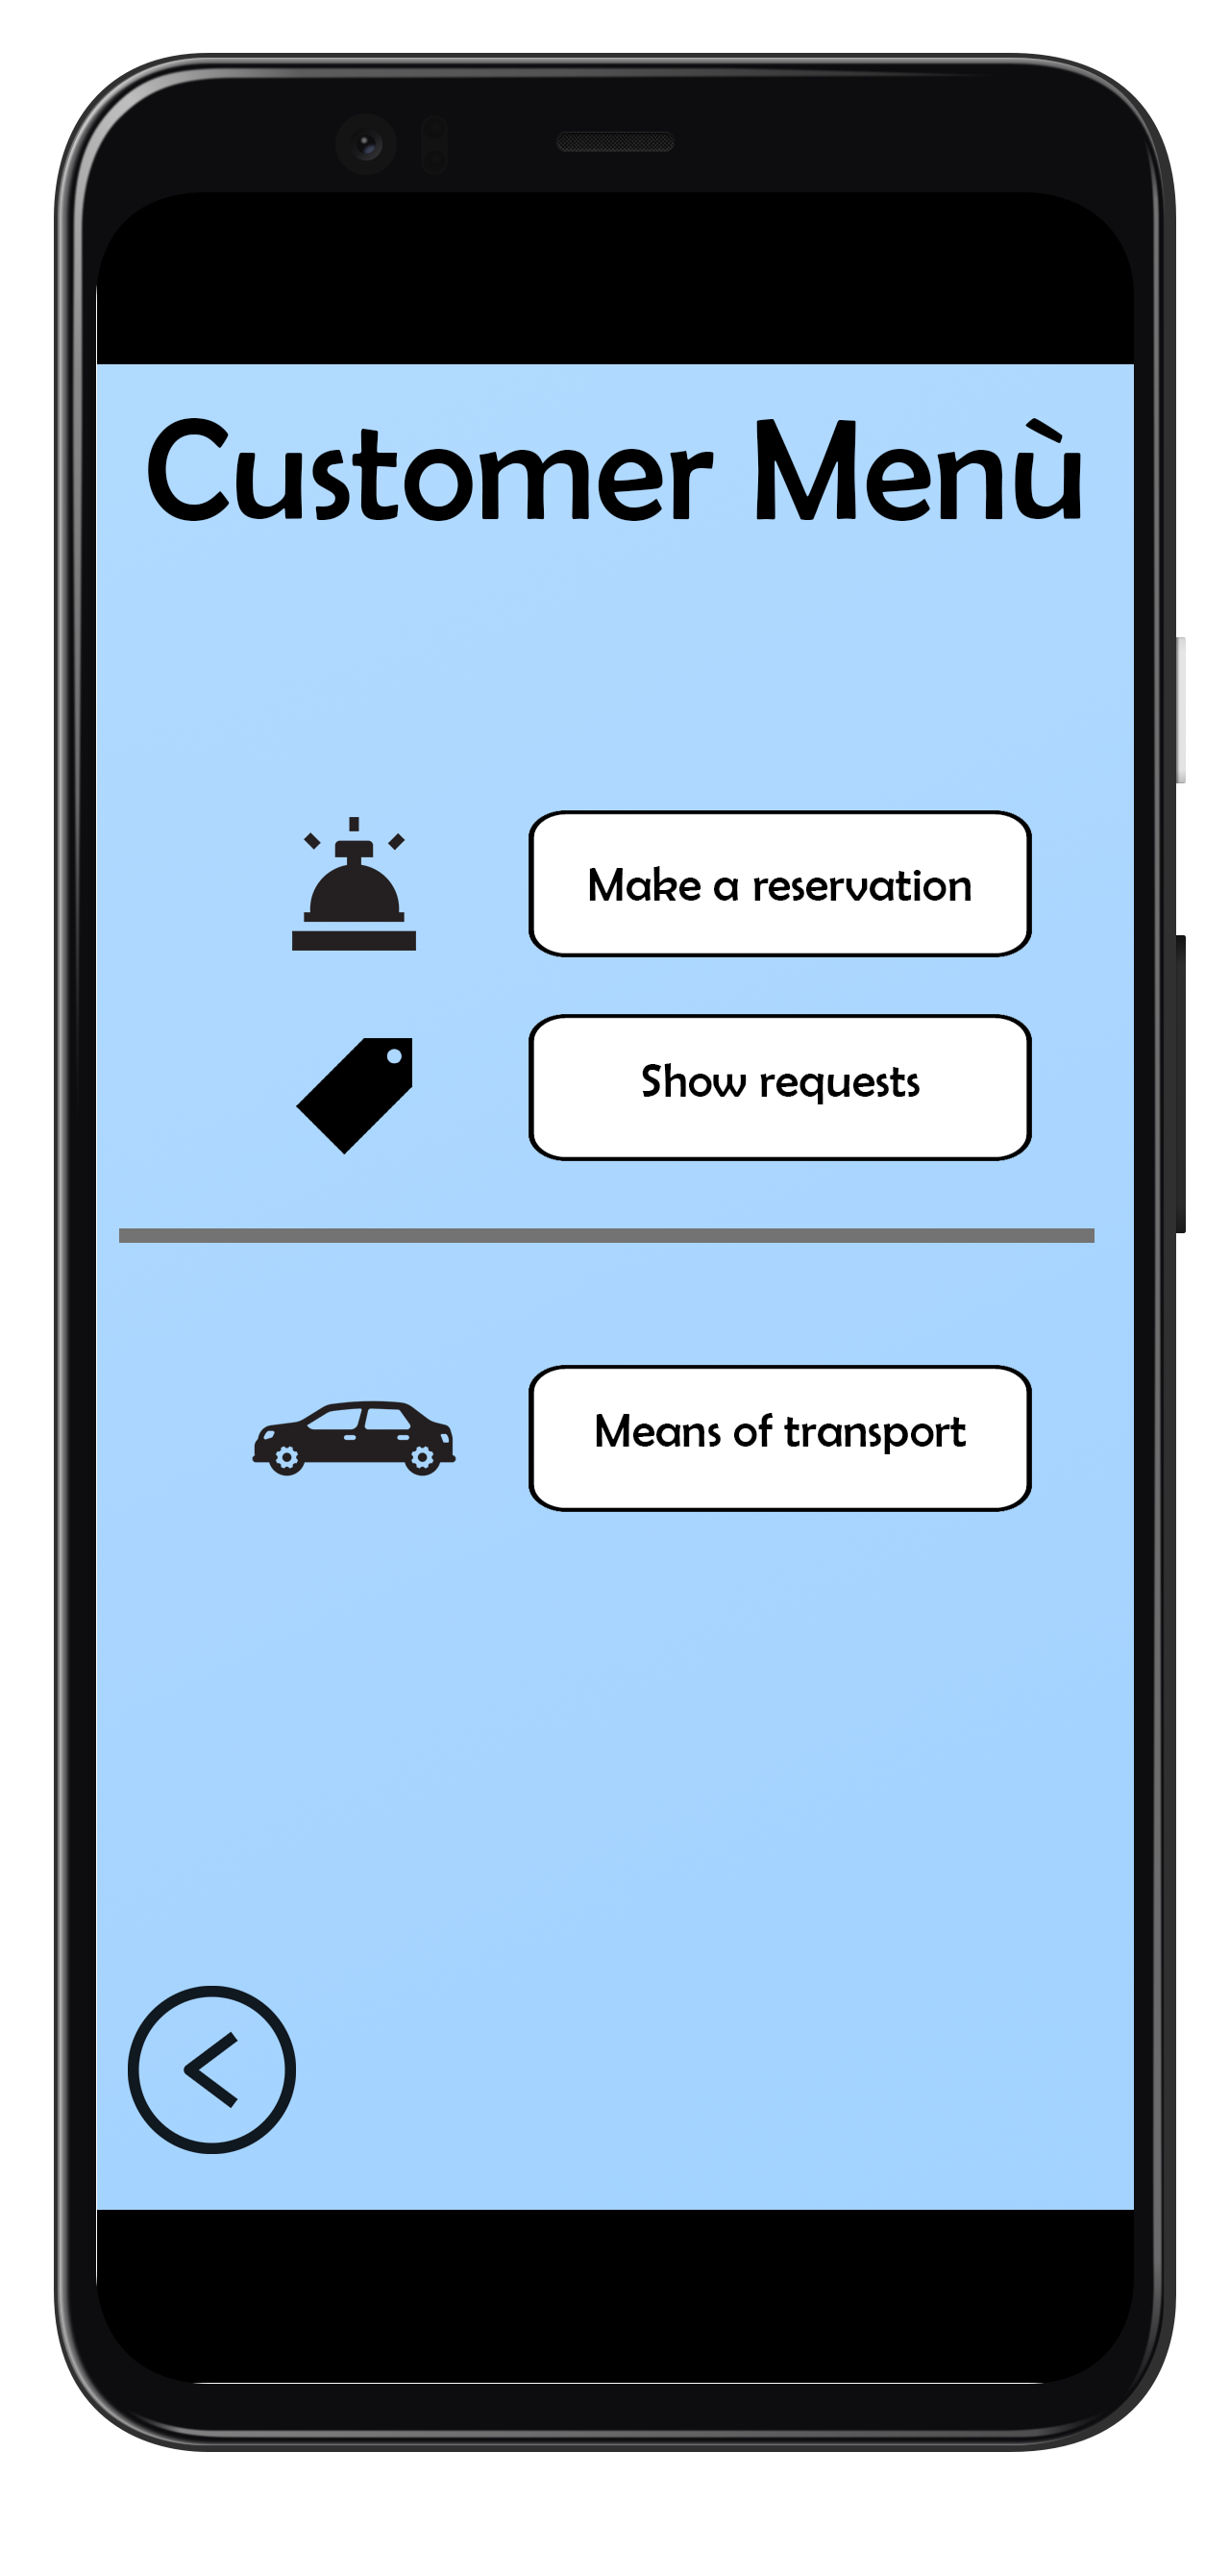
\includegraphics[width=\textwidth]{../Mockups/MenuCustomer.png}
				\caption{\emph{Customer menù}}
			\end{minipage}
			\hfill
			\begin{minipage}[!h]{0.4\textwidth}
				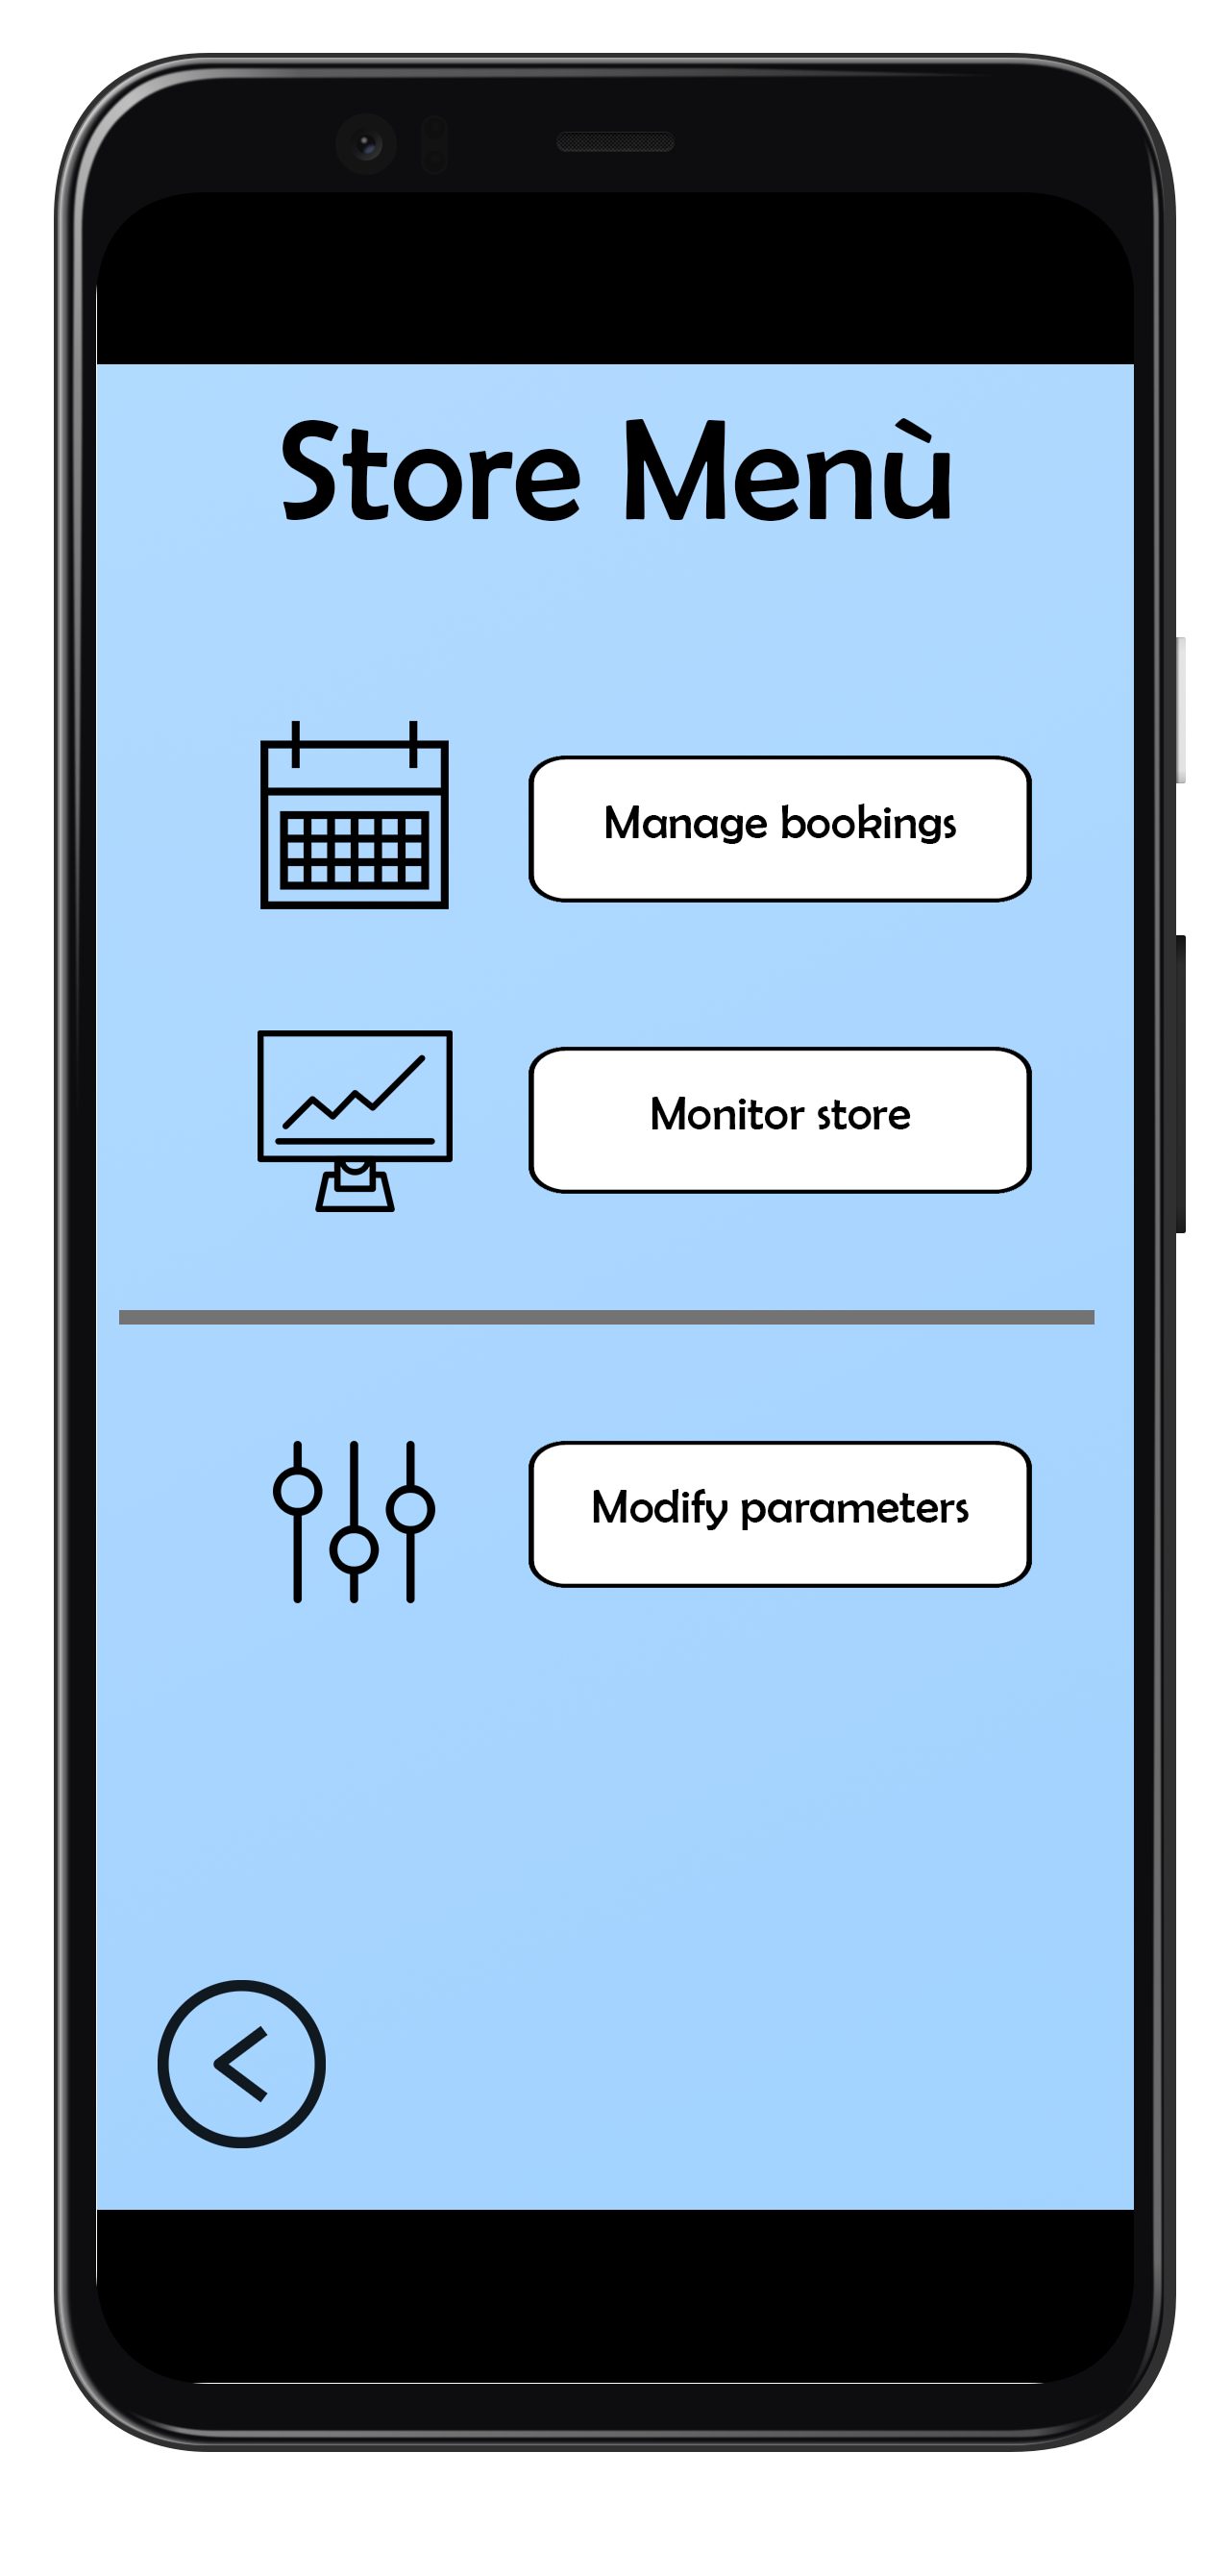
\includegraphics[width=\textwidth]{../Mockups/MenuStore.png}
				\caption{\emph{Store manager menù}}
			\end{minipage}
		\end{figure}		
		
		\newpage 
		
		\subsubsection{Make a reservation}
		In this section are shown the mockups about the booking of a reservation. When a customer wants to make a reservation have to select the store where he wants to make his purchases. The store, thanks to \emph{Maps API}, are ordered in ascending order by distance. After the selection, the customer can selected the products that he wants to purchase or, at least, the departments that he intends to visit during his purchases.
		\bigskip
		\bigskip
		\begin{figure}[!h]
			\centering
			\begin{minipage}[!h]{0.4\textwidth}
				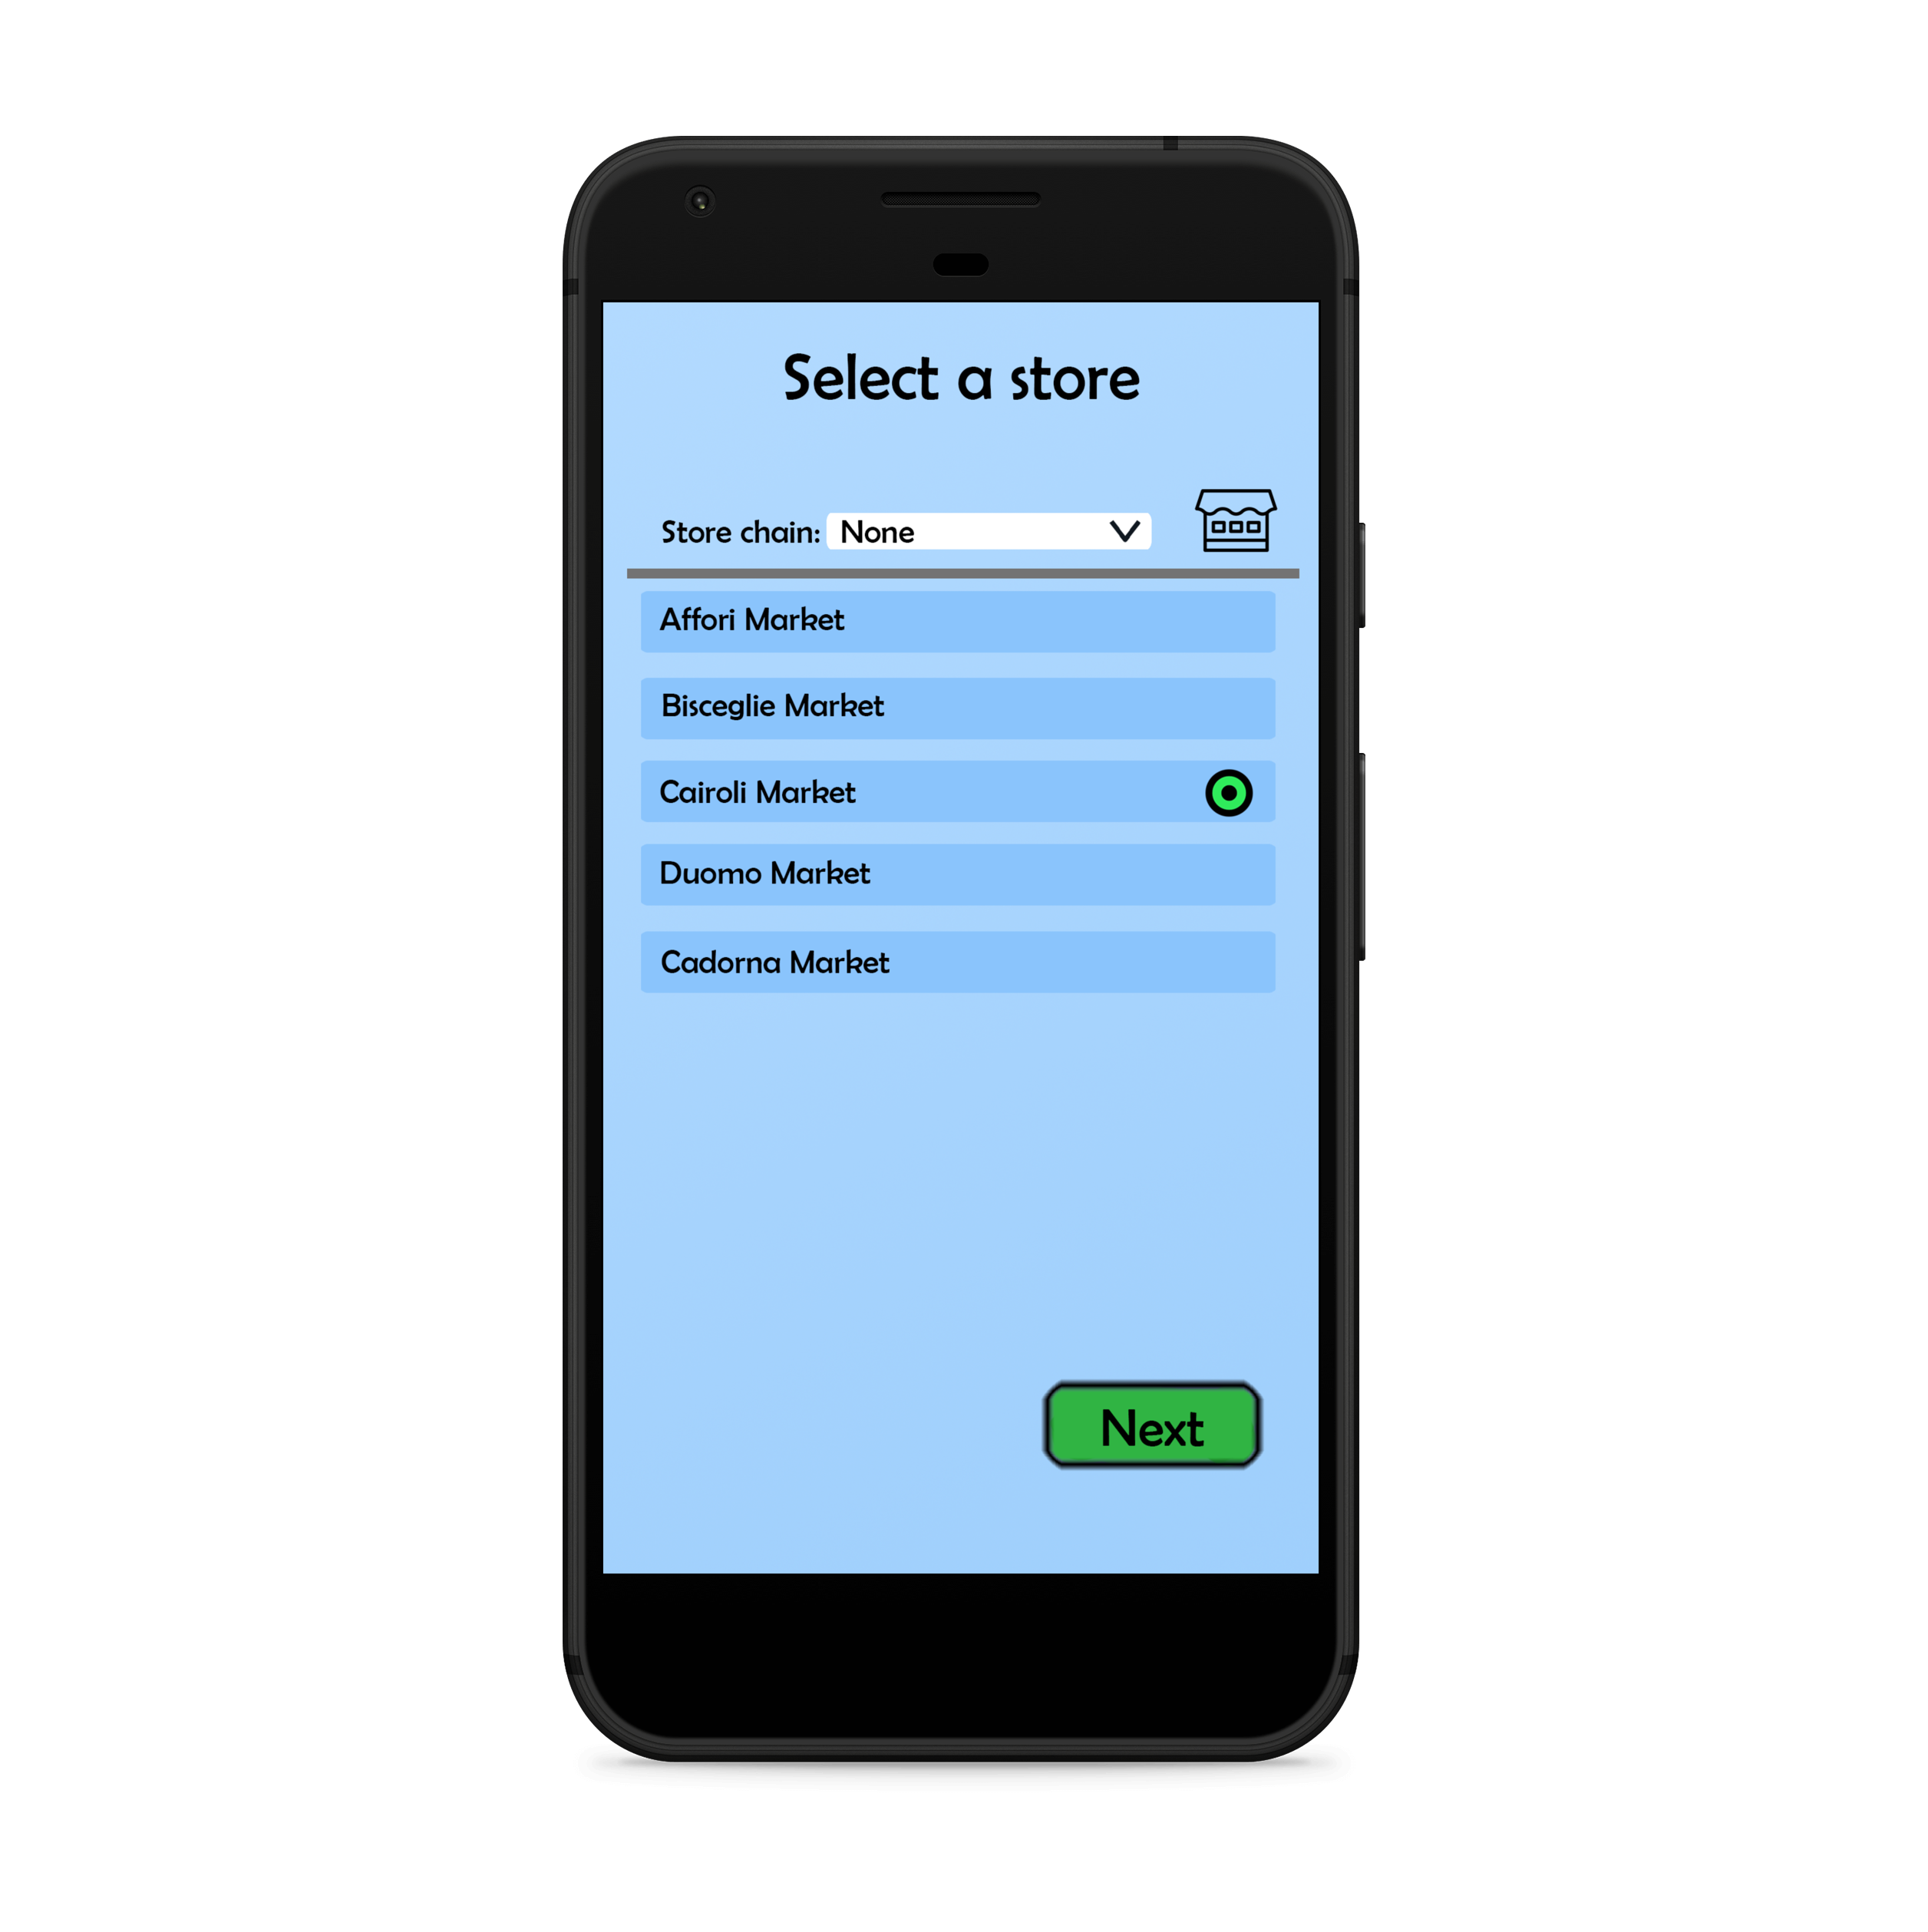
\includegraphics[width=\textwidth]{../Mockups/SelectStore.png}
				\caption{\emph{Store selection}}
			\end{minipage}
			\hfill
			\begin{minipage}[!h]{0.4\textwidth}
				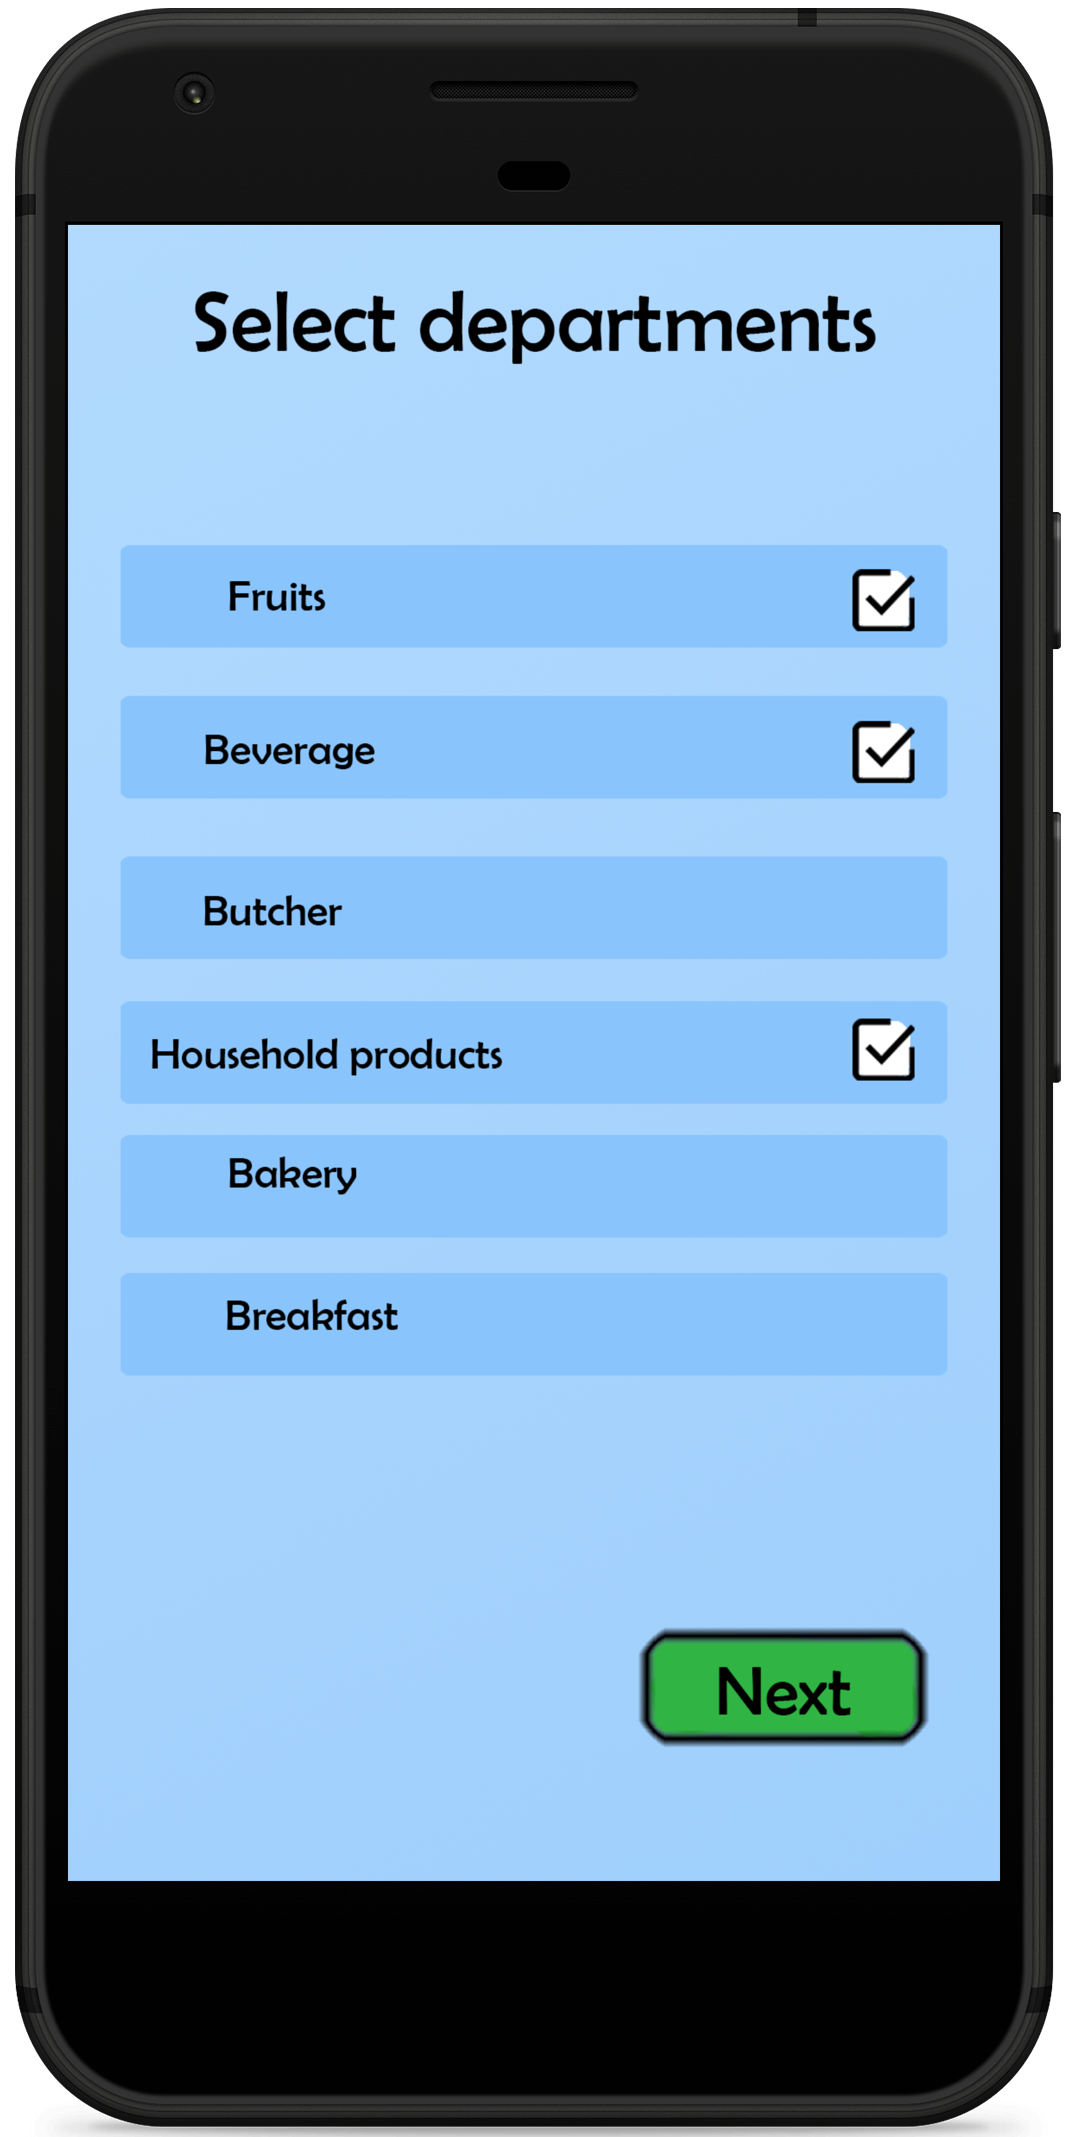
\includegraphics[width=\textwidth]{../Mockups/SelectDepartments.png}
				\caption{\emph{Departments selection}}
			\end{minipage}
		\end{figure}
		After this first phase, the customer can insert the estimation time of the duration of his expense. In case this parameter is not inserted by the customer, the system will calculate a reasonable estimation time with two criteria, based on the situation:
		\begin{itemize}
			\item In case of the system have sufficient data about customer, it provided to calculate the estimation time based on customer's previous expenses.
			\item In case of the system does not have sufficient data about customer, it provides to calculate the estimation time based on the data of other customers who have made a similar expense, referring to the departments that the customer has previously selected.
		\end{itemize}
	
		Then, the customer must select the reservation type which can be of two types:
		\begin{itemize}
			\item {\bfseries ASAP}: In this case the customer will be placed inside the queue occupying the first available slot.
			\item {\bfseries Choose Slot}: In this case the customer is going to select an available slot with a length equal to the duration entered or calculated previously.
		\end{itemize}
		\bigskip
		\bigskip
		\begin{figure}[!h]
			\centering
			\begin{minipage}[!h]{0.4\textwidth}
				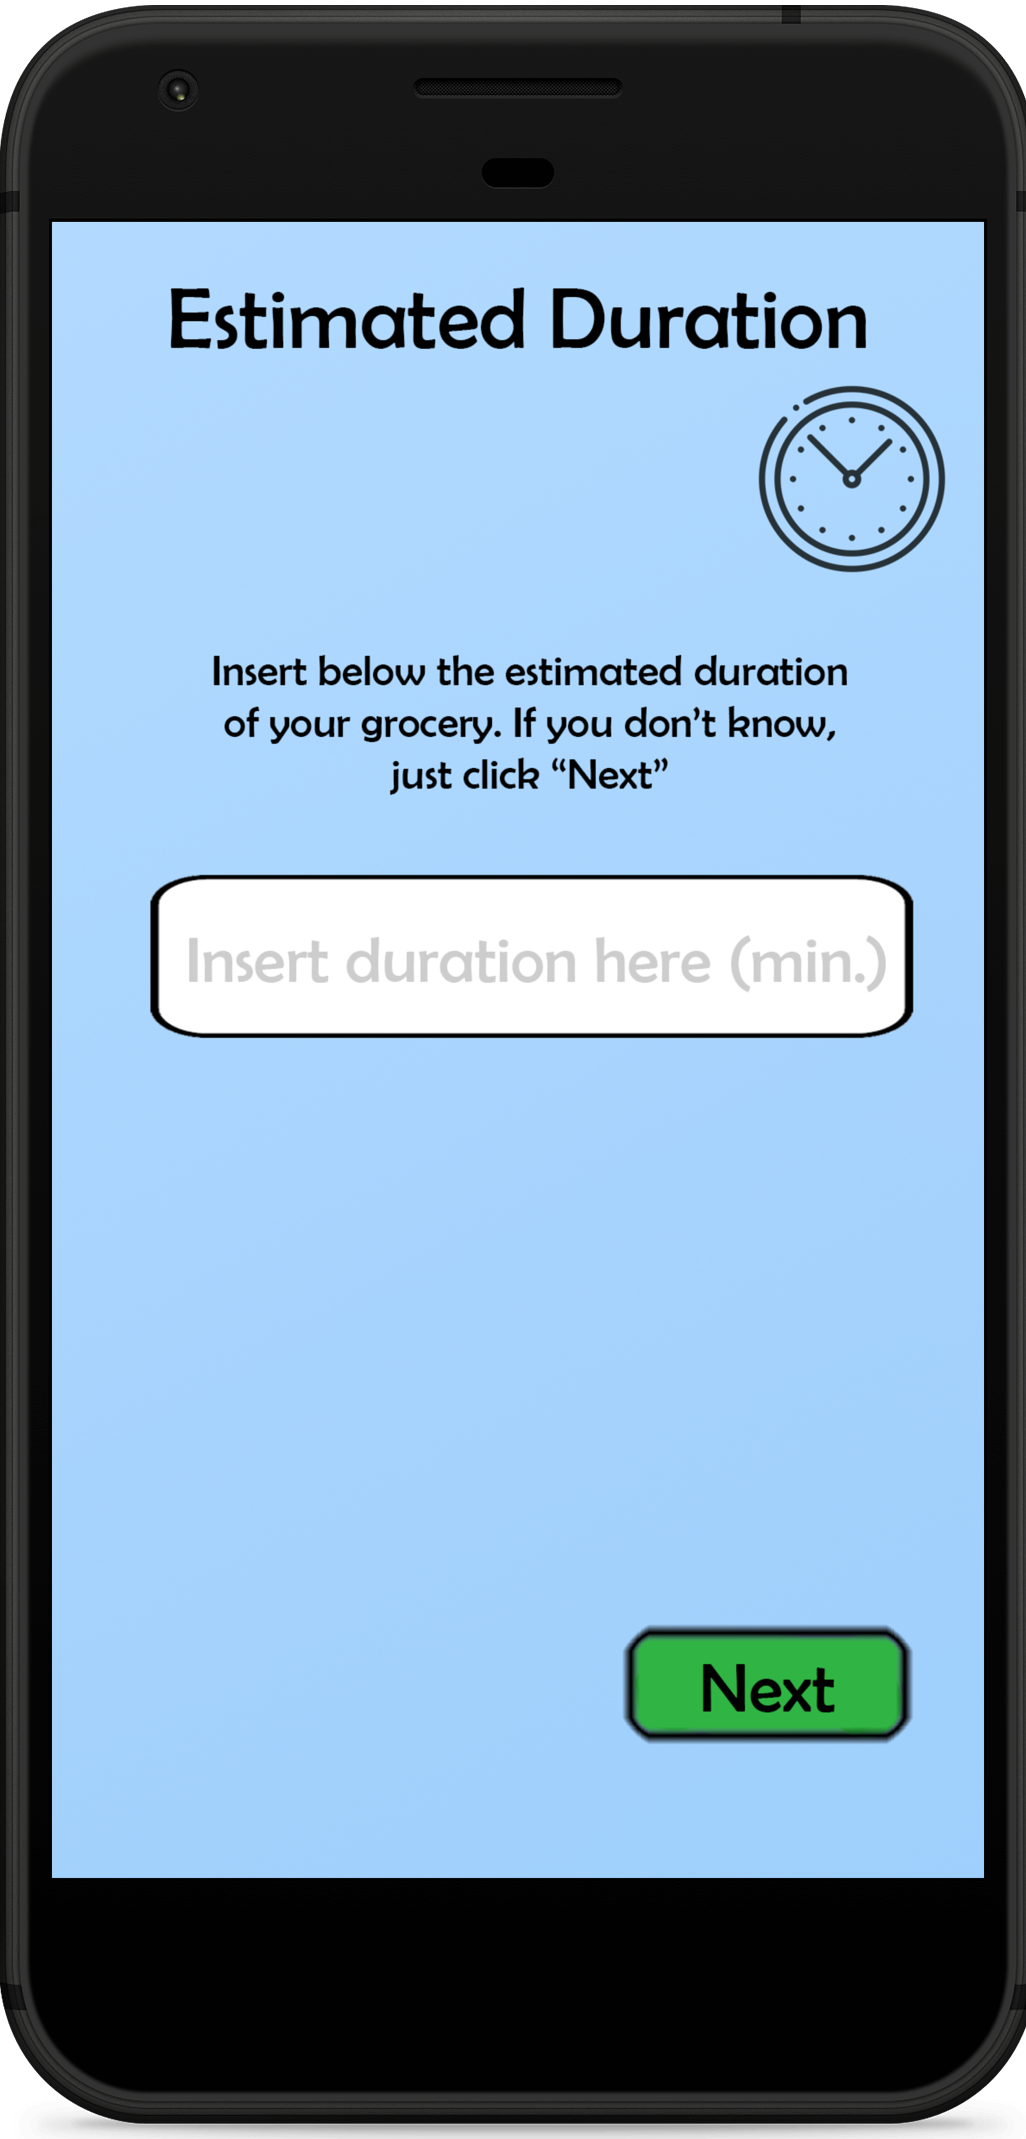
\includegraphics[width=\textwidth]{../Mockups/EstimatedDuration.png}
				\caption{\emph{Estimated duration}}
			\end{minipage}
			\hfill
			\begin{minipage}[!h]{0.4\textwidth}
				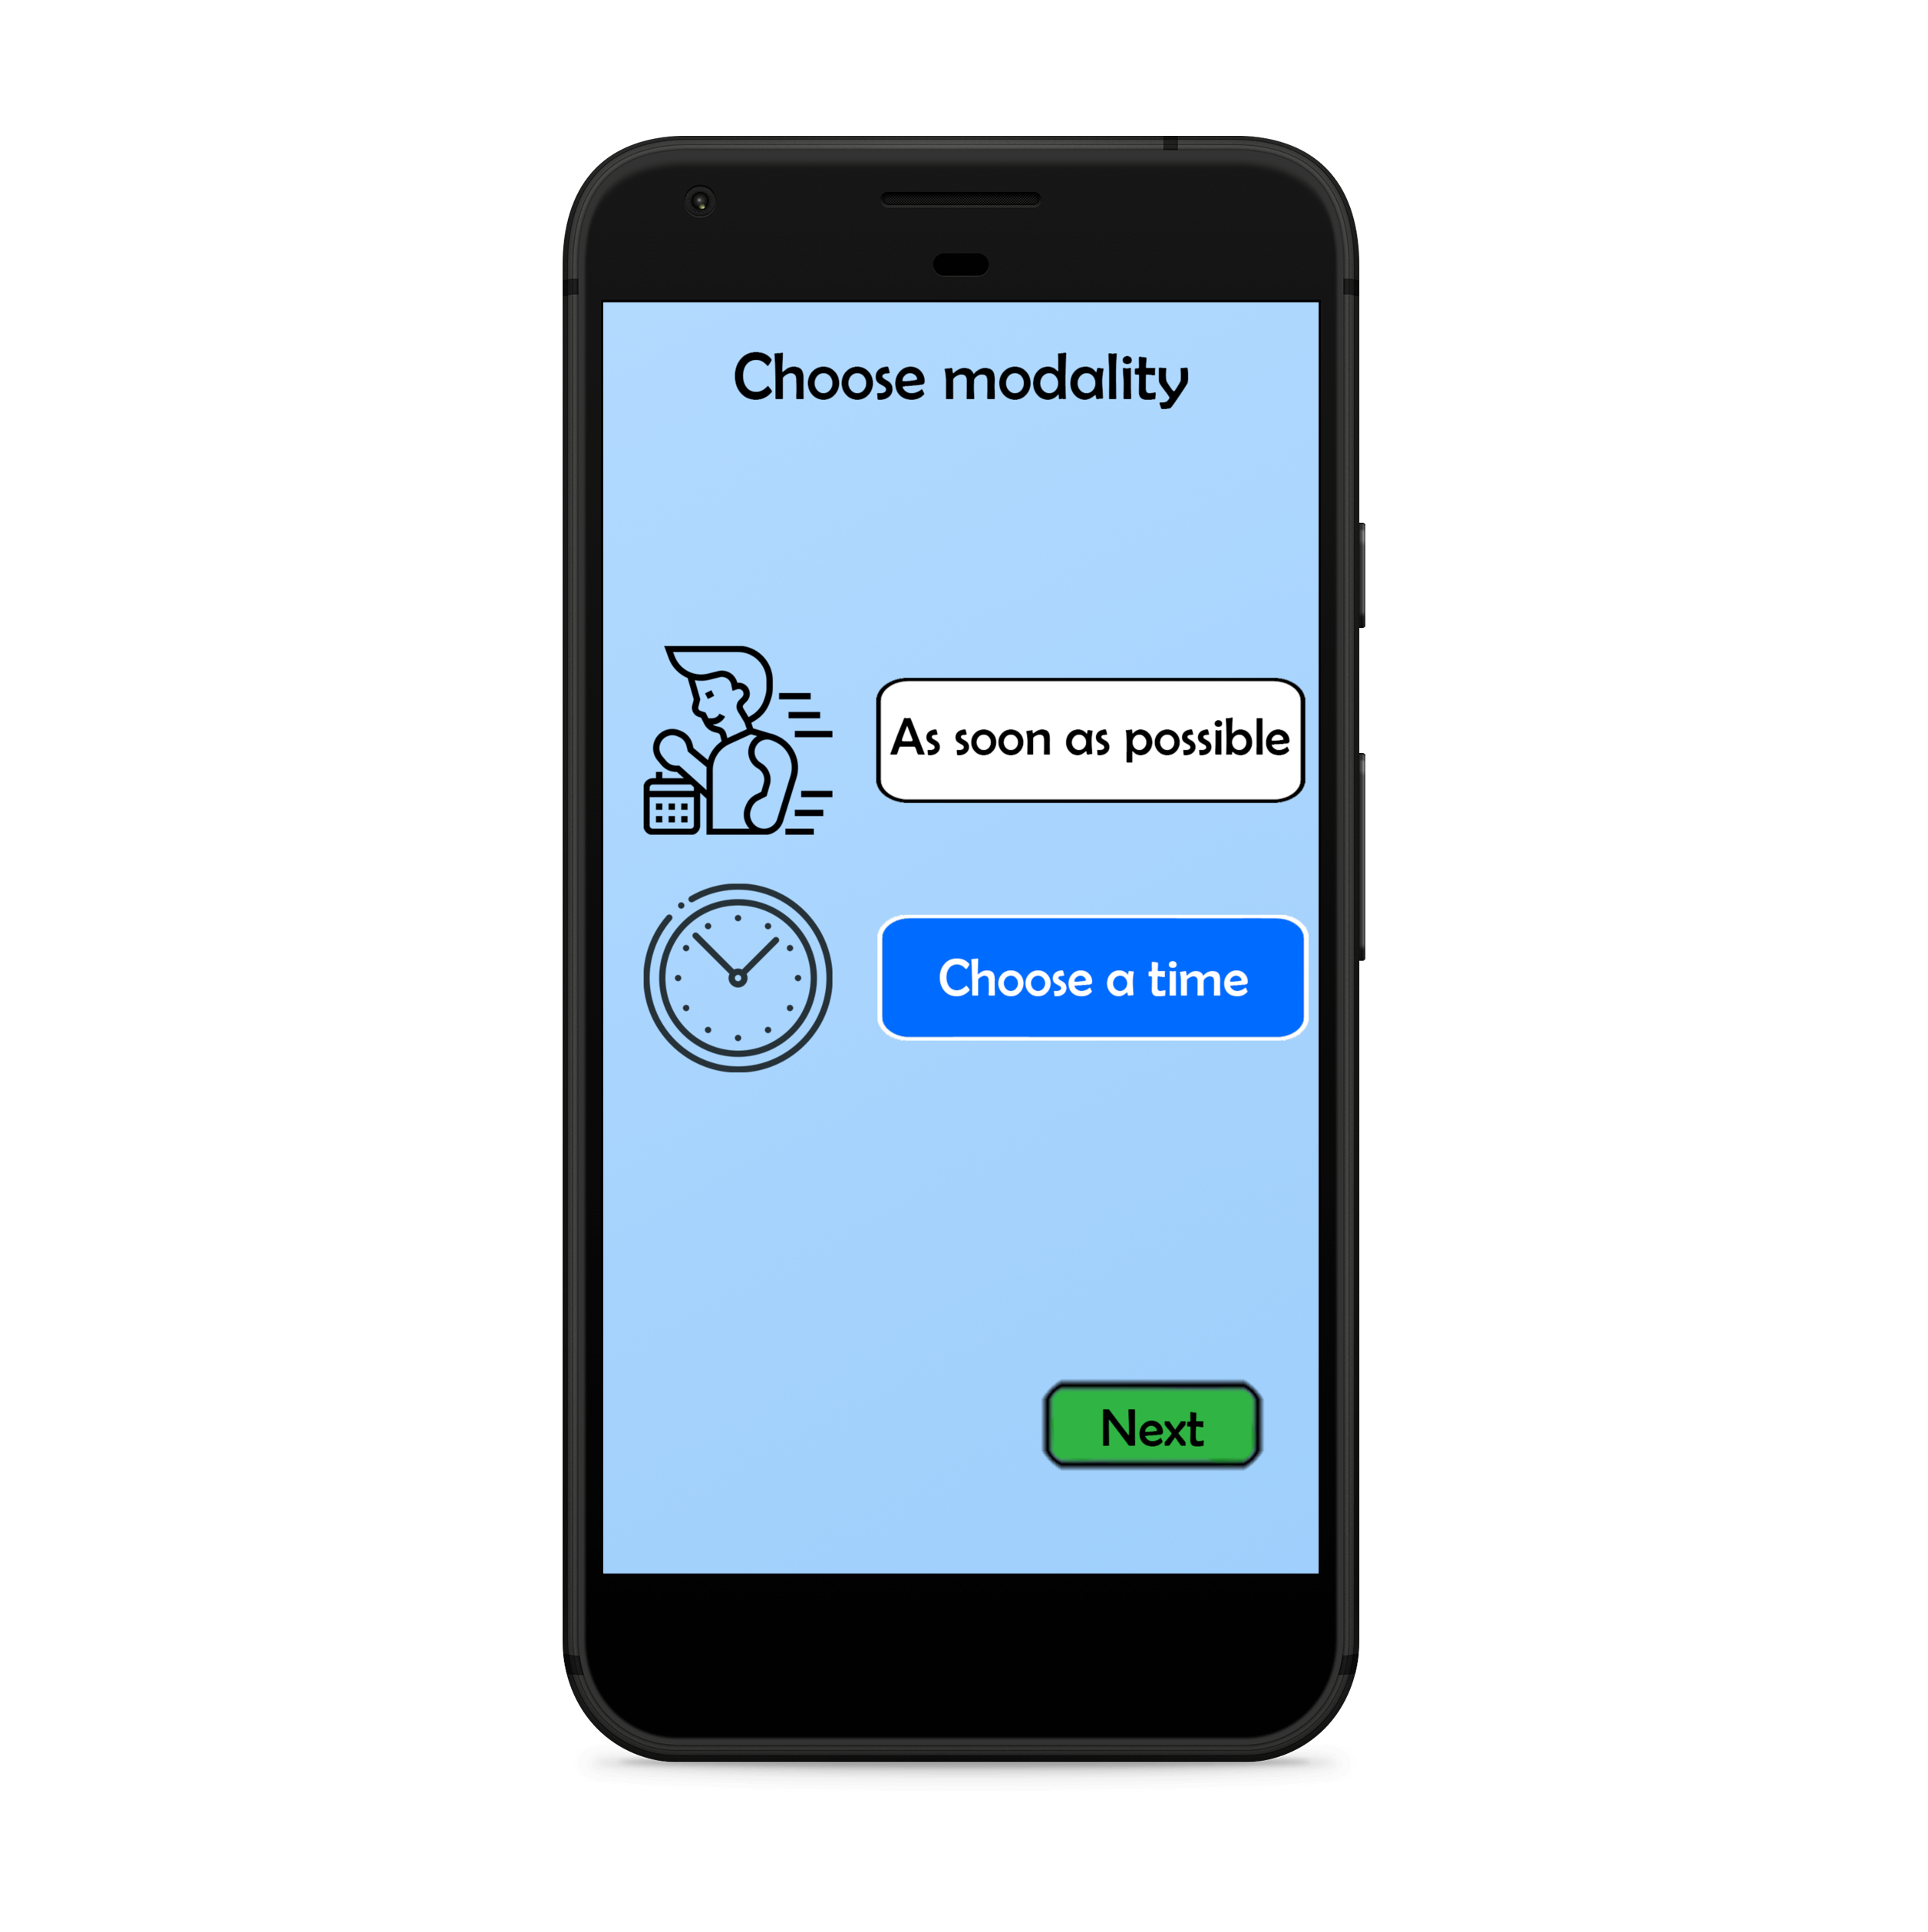
\includegraphics[width=\textwidth]{../Mockups/ChooseModality.png}
				\caption{\emph{Choice of reservation type}}
			\end{minipage}
		\end{figure}
	
		\newpage
		
		\subsubsection{Choose Slot}
		In this section is shown the mockup about the choice of time slot. If a customer decide to plan a visit to the store, he must select a time slot which indicates the time spent by the customer inside the store. The customer can complete his reservation, but, in case of he is not fully satisfied with the time slots, he can asks for suggestions.
		\bigskip
		\bigskip
		\begin{figure}[!h]
 			\begin{adjustwidth} {0cm}{}
				\centering
				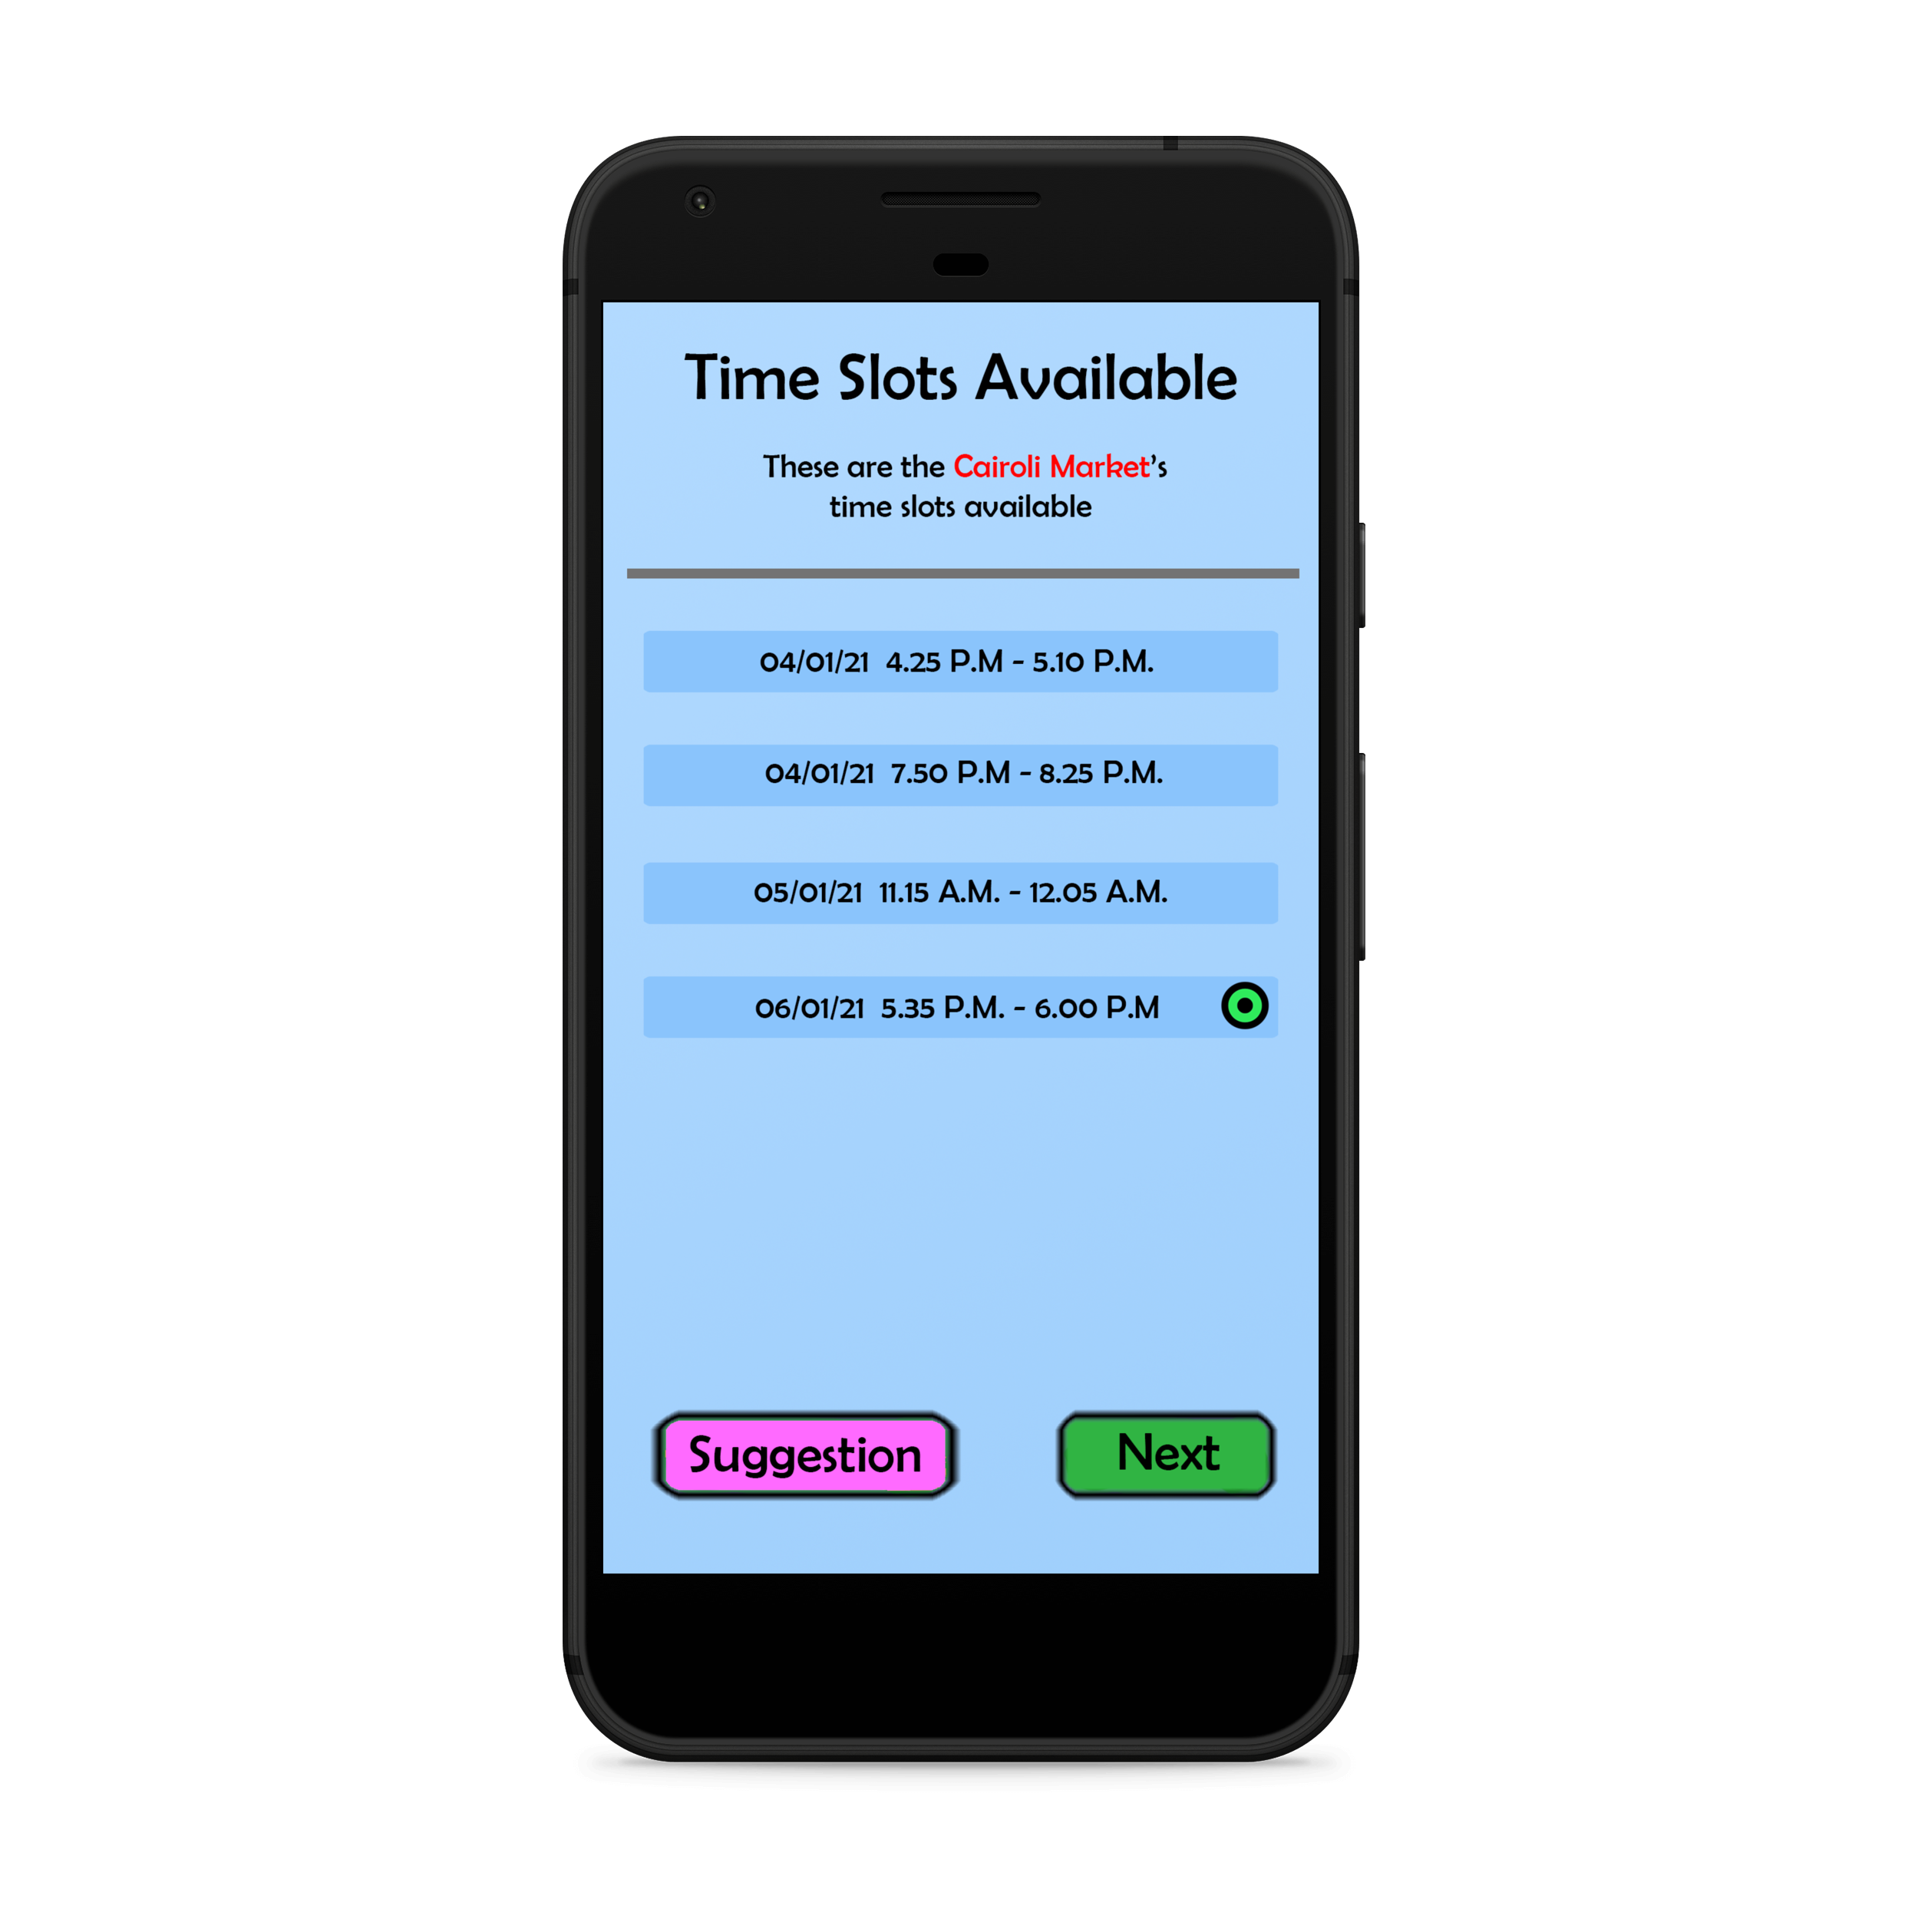
\includegraphics[scale=0.2]{../Mockups/TimeSlots.png}\\
			\end{adjustwidth}
			\caption{\emph{Time slots}}
		\end{figure}
		
		\newpage
		
		\subsubsection{Suggestions}
		In this section is shown the mockups about the suggestions of a reservation. If a customer is not satisfied with the available time slots the app allows to receive suggestions. These one are different based on the type of reservation selected previously:
		\begin{itemize}
			\item In case of customer has selected an \emph{ASAP} reservation, if the wait is very long, suggestions are shown automatically. In this case are show, in order of waiting, all the stores that have a better time slot available (including the chosen one) and the customer can accept one of the suggestion or select again the initial store.
			\item In case of customer has planned a visit but the time slots do not fully satisfy him, he can select a new store, ordered from best to worst, and see the time slots of these new stores. When the customer identify the better choice for him, he can complete the reservation.
		\end{itemize}
		\bigskip
		\begin{figure}[!h]
			\centering
			\begin{minipage}[!h]{0.4\textwidth}
				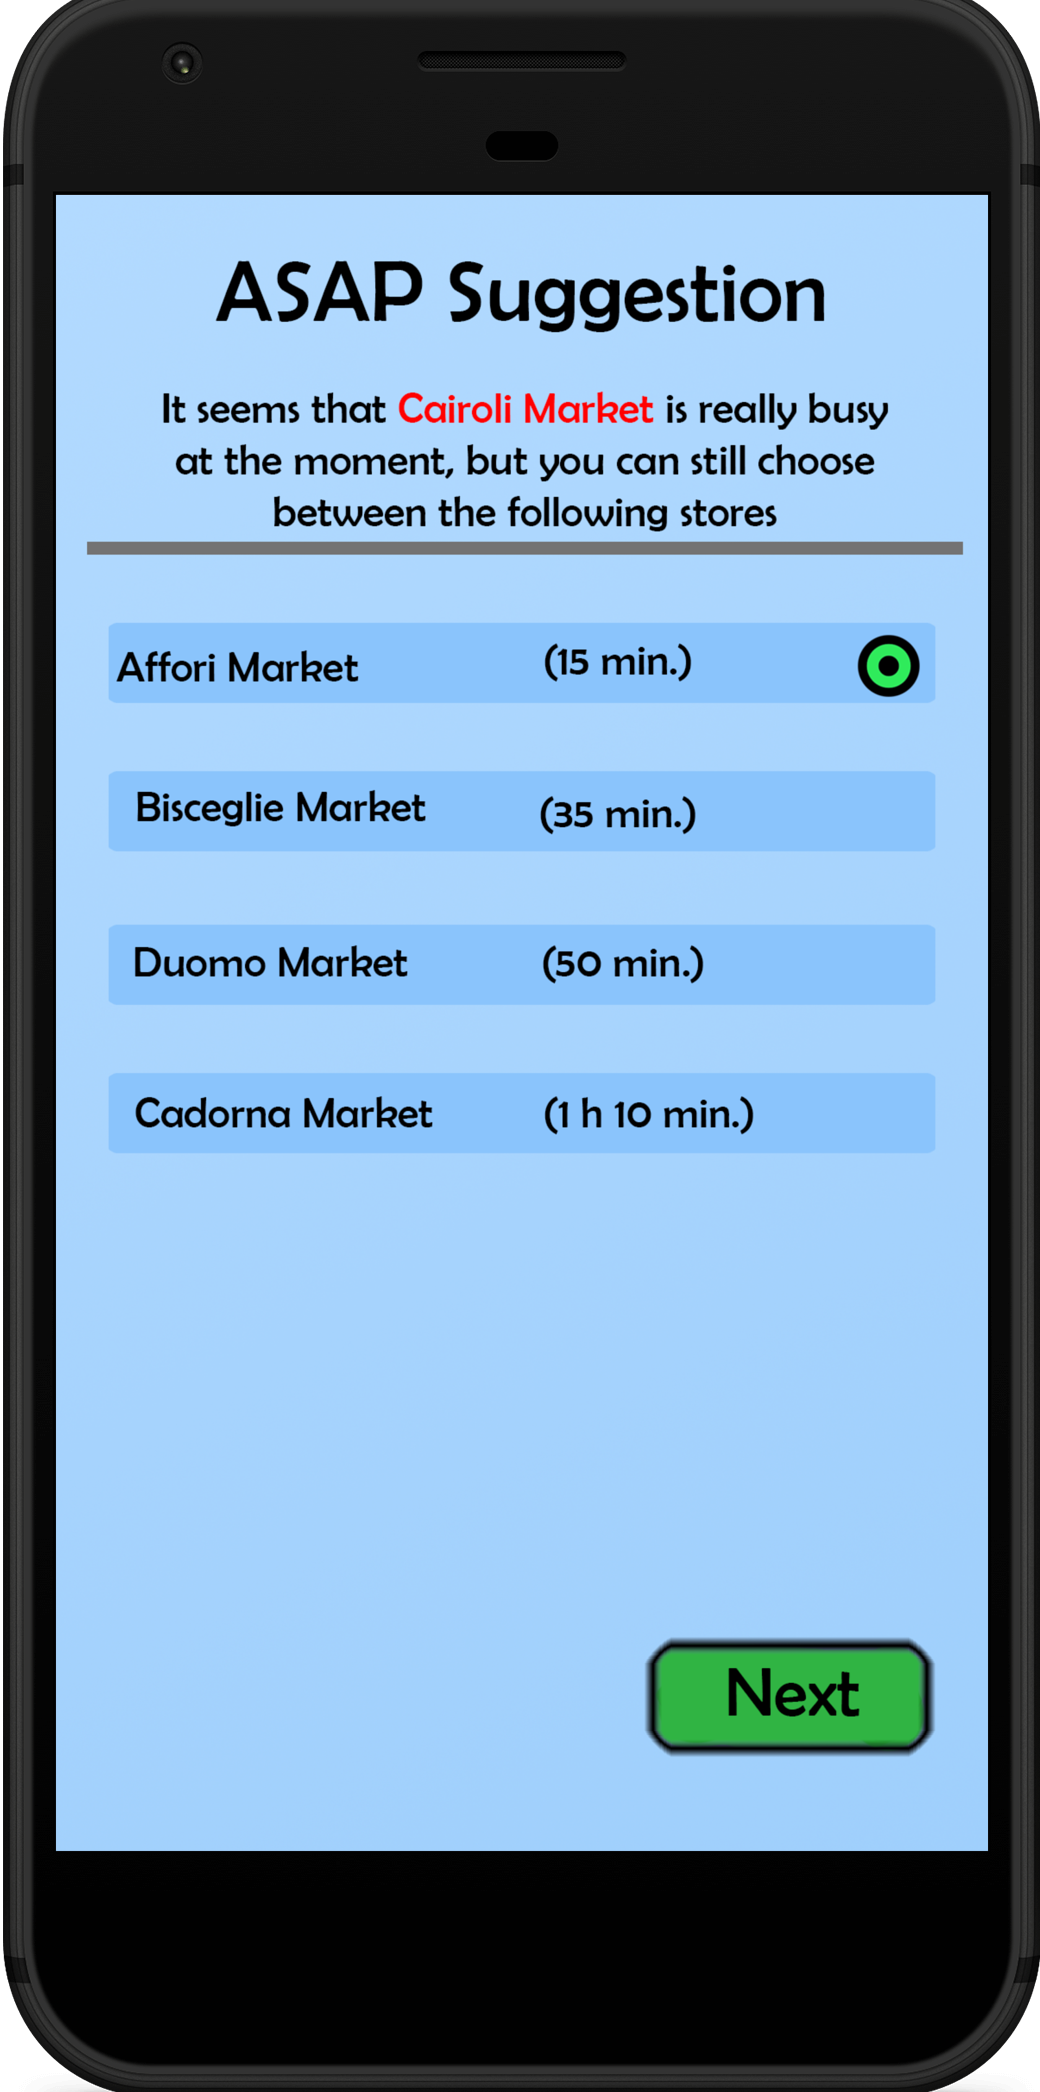
\includegraphics[width=\textwidth]{../Mockups/ASAPSuggestion.png}
				\caption{\emph{ASAP suggestion}}
			\end{minipage}
			\hfill
			\begin{minipage}[!h]{0.4\textwidth}
				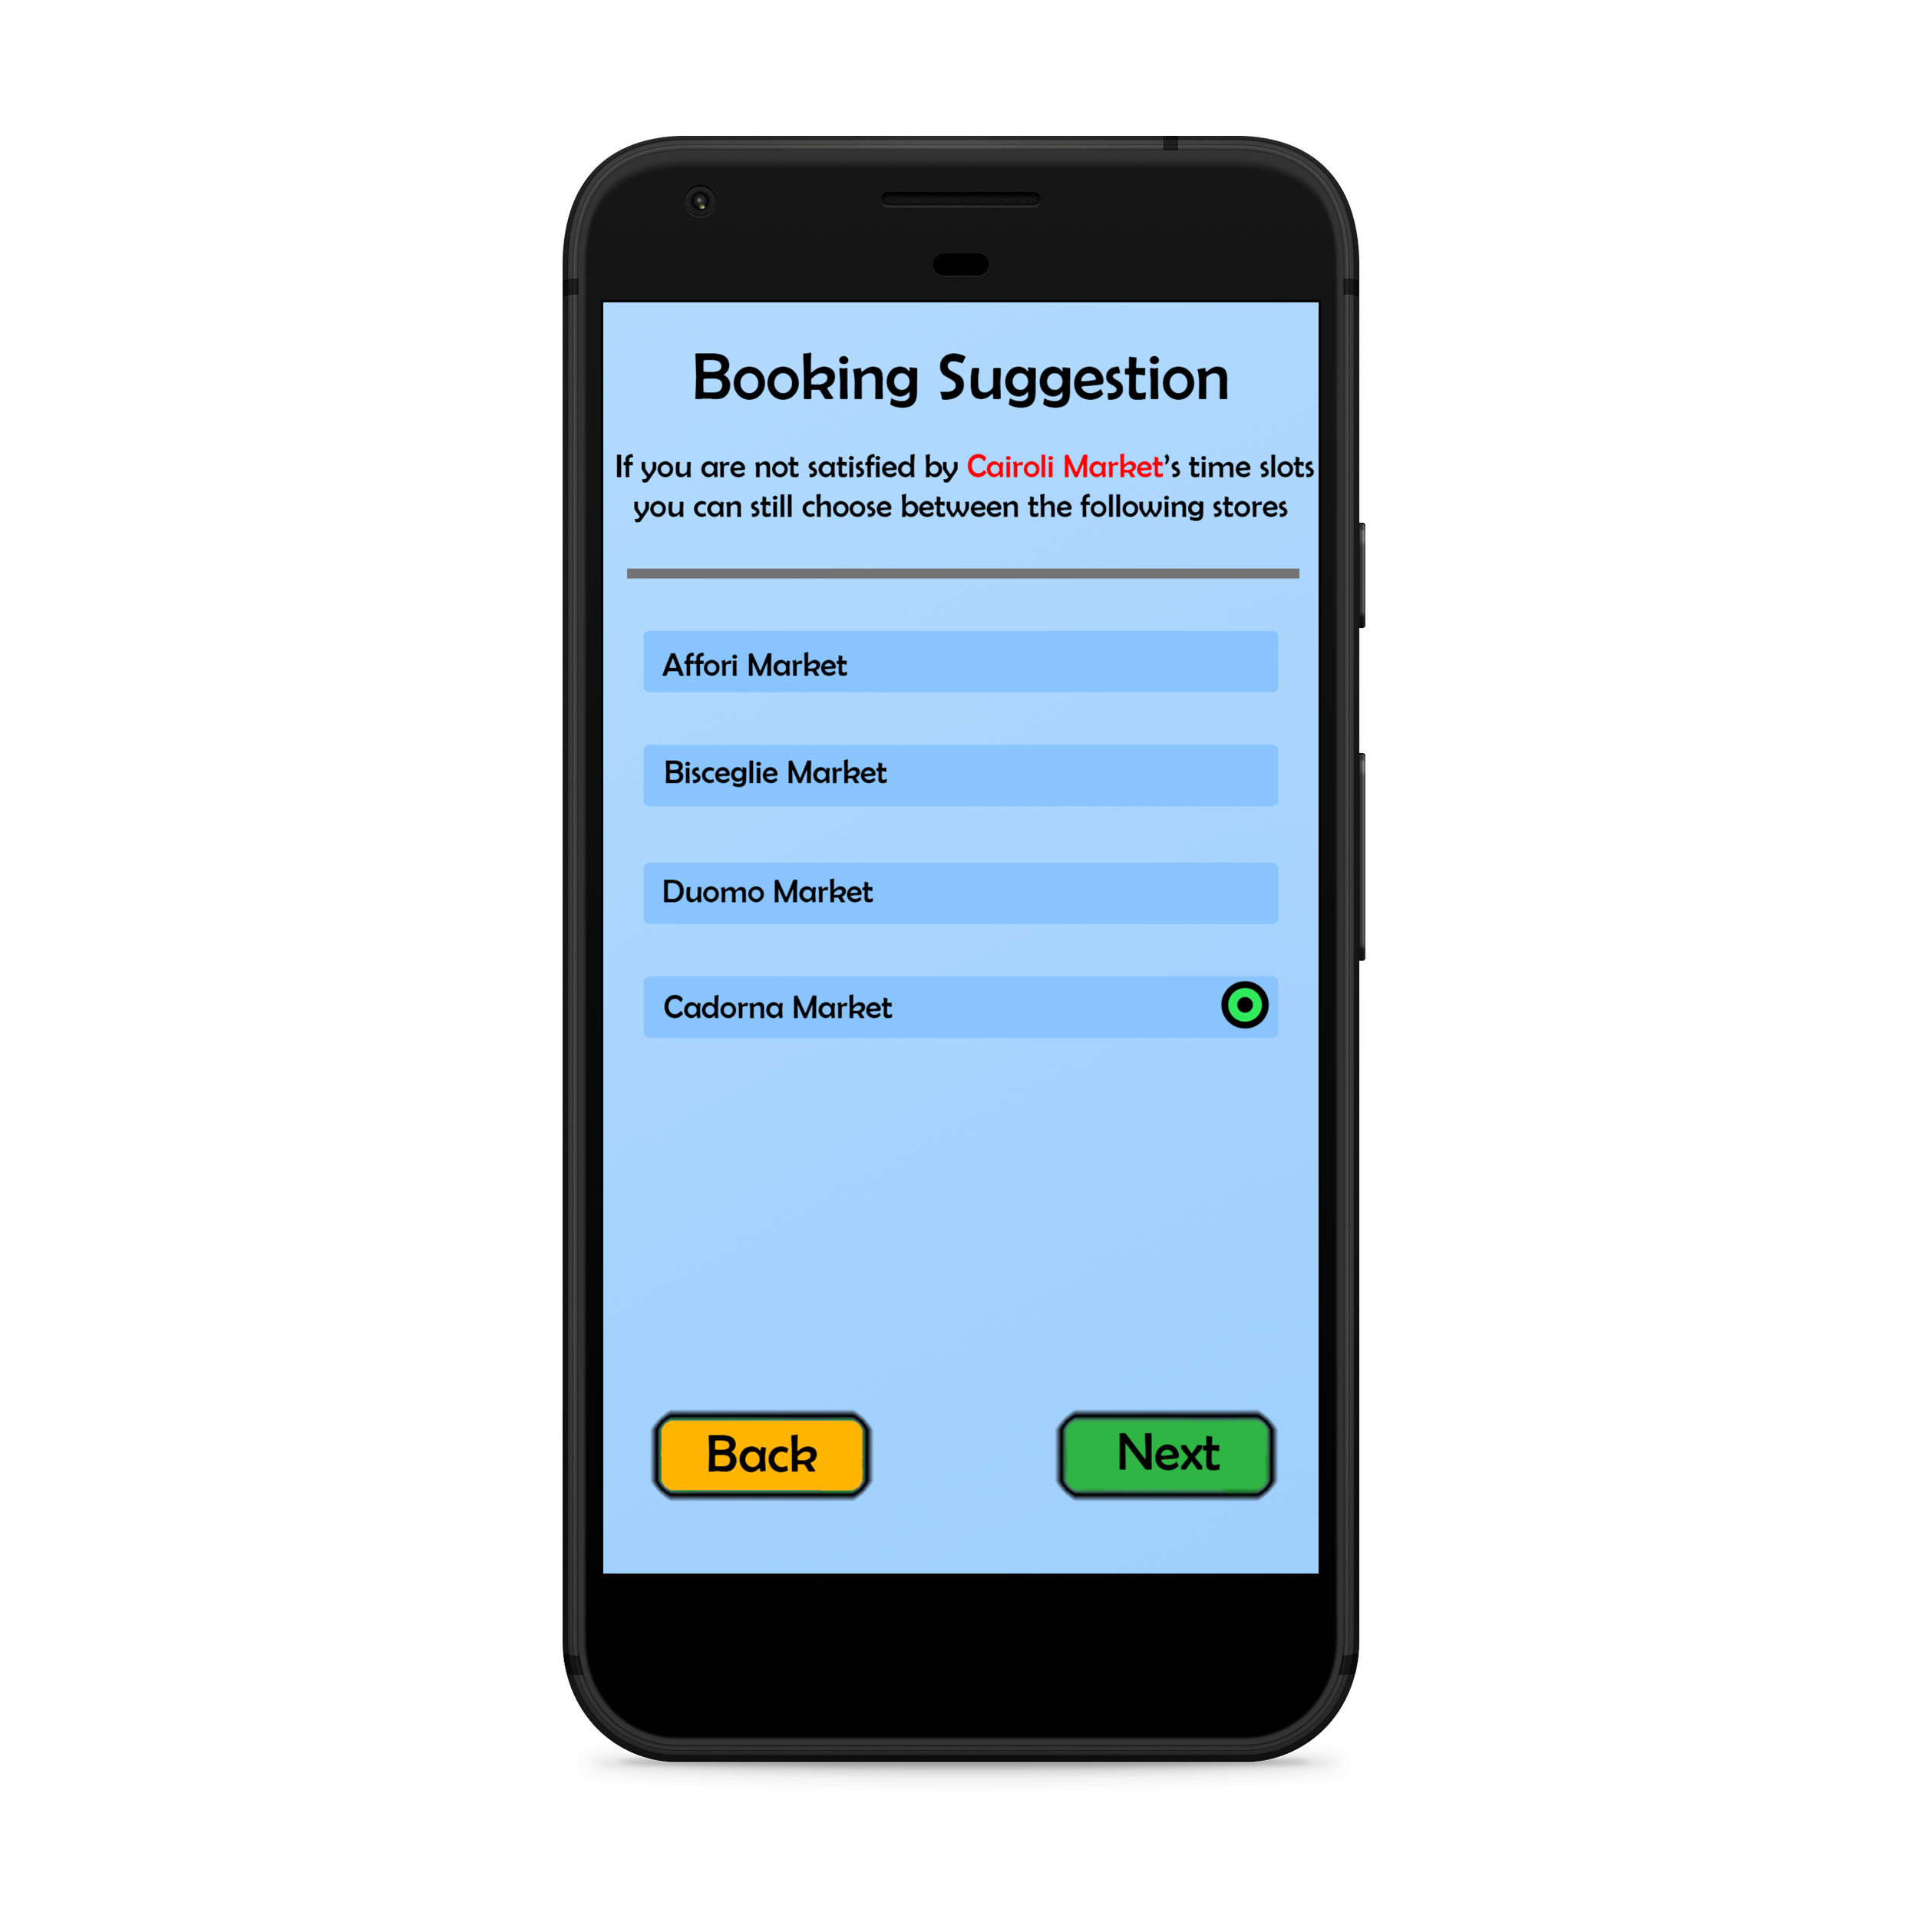
\includegraphics[width=\textwidth]{../Mockups/BookingSuggestion.png}
				\caption{\emph{Reservation suggestion}}
			\end{minipage}
		\end{figure}
	
		\newpage
		
		\subsubsection{Ticket}
		In this section are shown the mockups about the ticket reservation. When the customer terminates his reservation, a ticket with a \emph{QR Code} is generated and saved. The ticket is used for enter and exit from the store and for both reservations it is the same. the only difference is that in the \emph{ASAP} one the entrance time is updated in real time.
		\bigskip
		\bigskip
		\begin{figure}[!h]
			\centering
			\begin{minipage}[!h]{0.4\textwidth}
				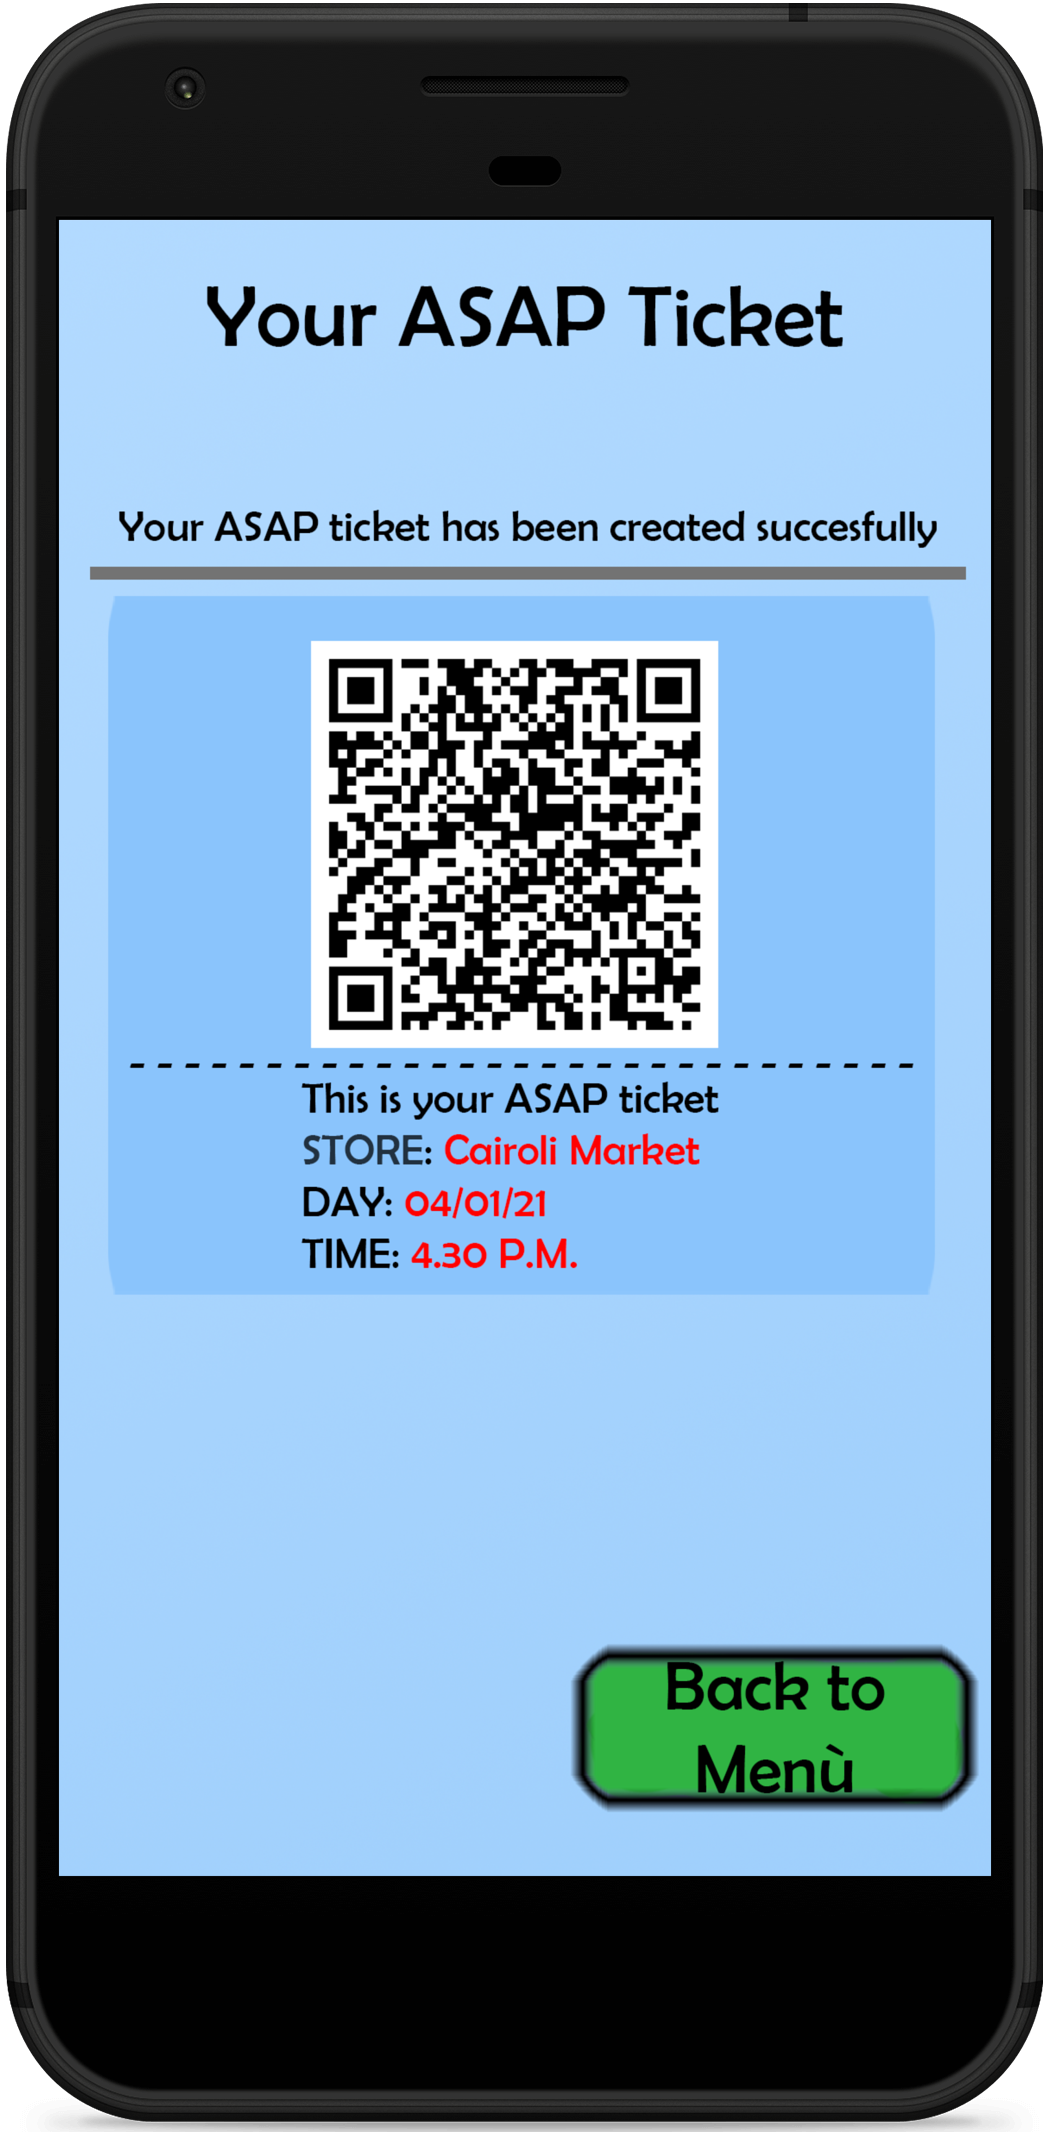
\includegraphics[width=\textwidth]{../Mockups/ASAPTicket.png}
				\caption{\emph{ASAP ticket}}
			\end{minipage}
			\hfill
			\begin{minipage}[!h]{0.4\textwidth}
				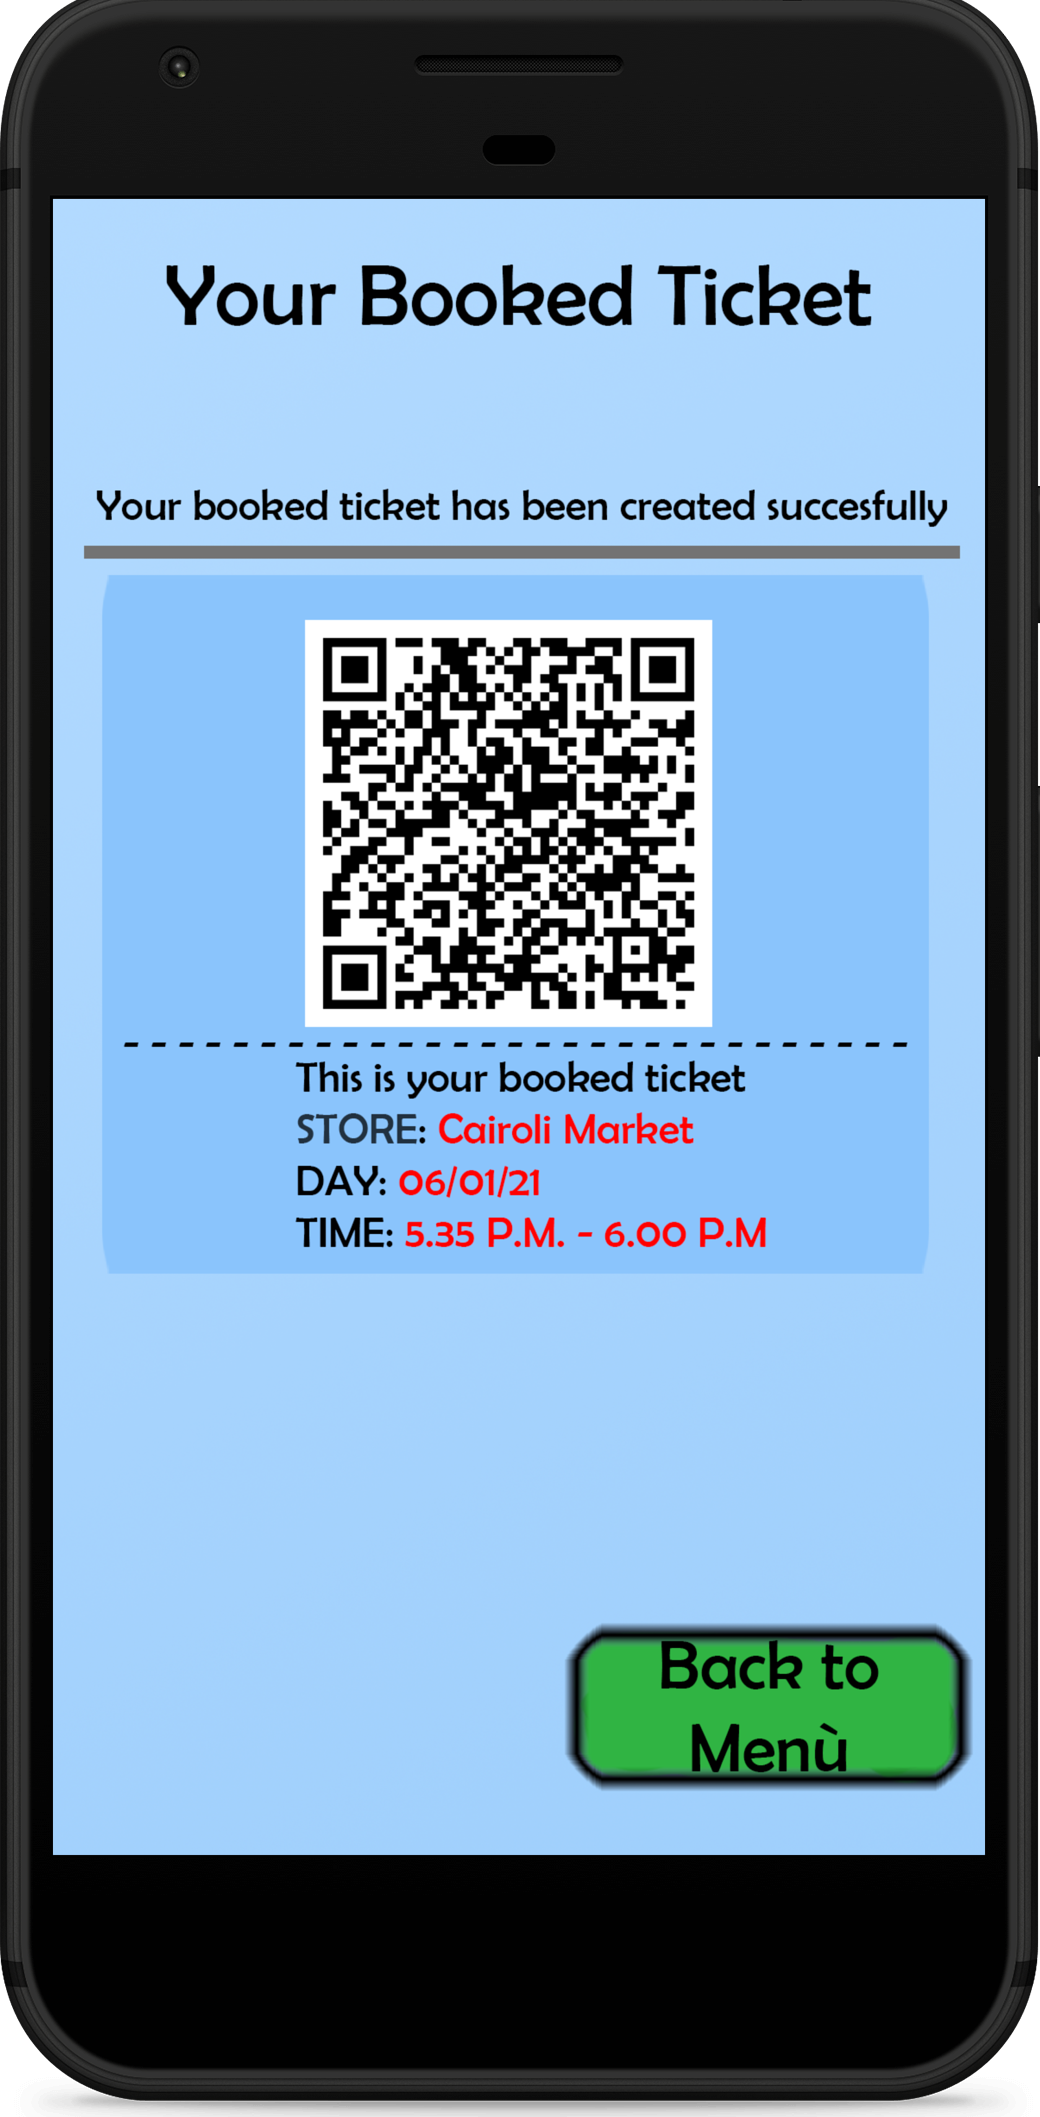
\includegraphics[width=\textwidth]{../Mockups/BookedTicket.png}
				\caption{\emph{Reservation ticket}}
			\end{minipage}
		\end{figure}
	
		\newpage
		
		\subsubsection{Visualize Booking}
		In this section are shown the mockups about the visualization of previous reservation. When the customer wants can see the previous reservation that he made. This functionality helps customer to build a detailed history.\\		\bigskip
		\bigskip
		\begin{figure}[!h]
			\centering
			\begin{minipage}[!h]{0.4\textwidth}
				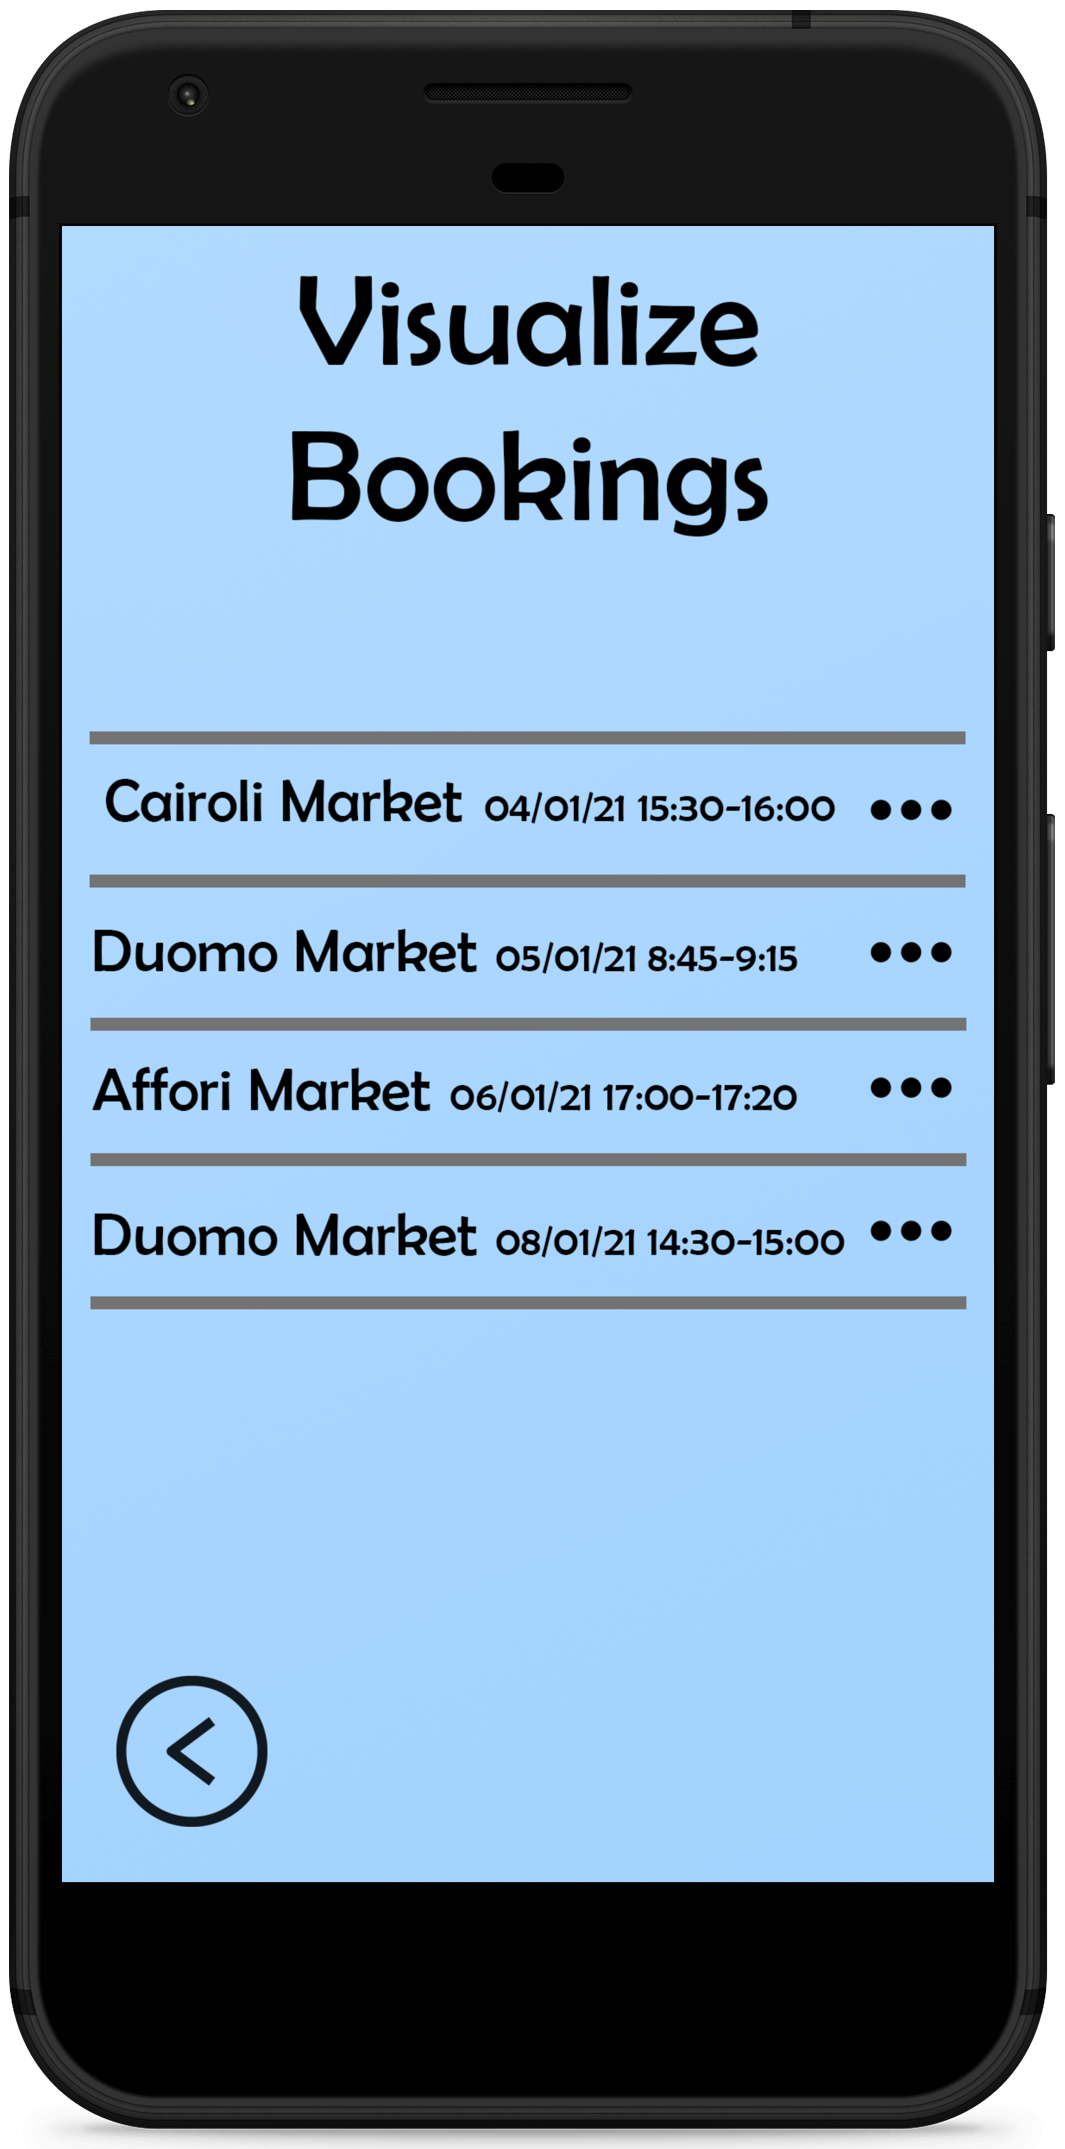
\includegraphics[width=\textwidth]{../Mockups/VisualizeBookings.png}
				\caption{\emph{Visualize reservations}}
			\end{minipage}
			\hfill
			\begin{minipage}[!h]{0.4\textwidth}
				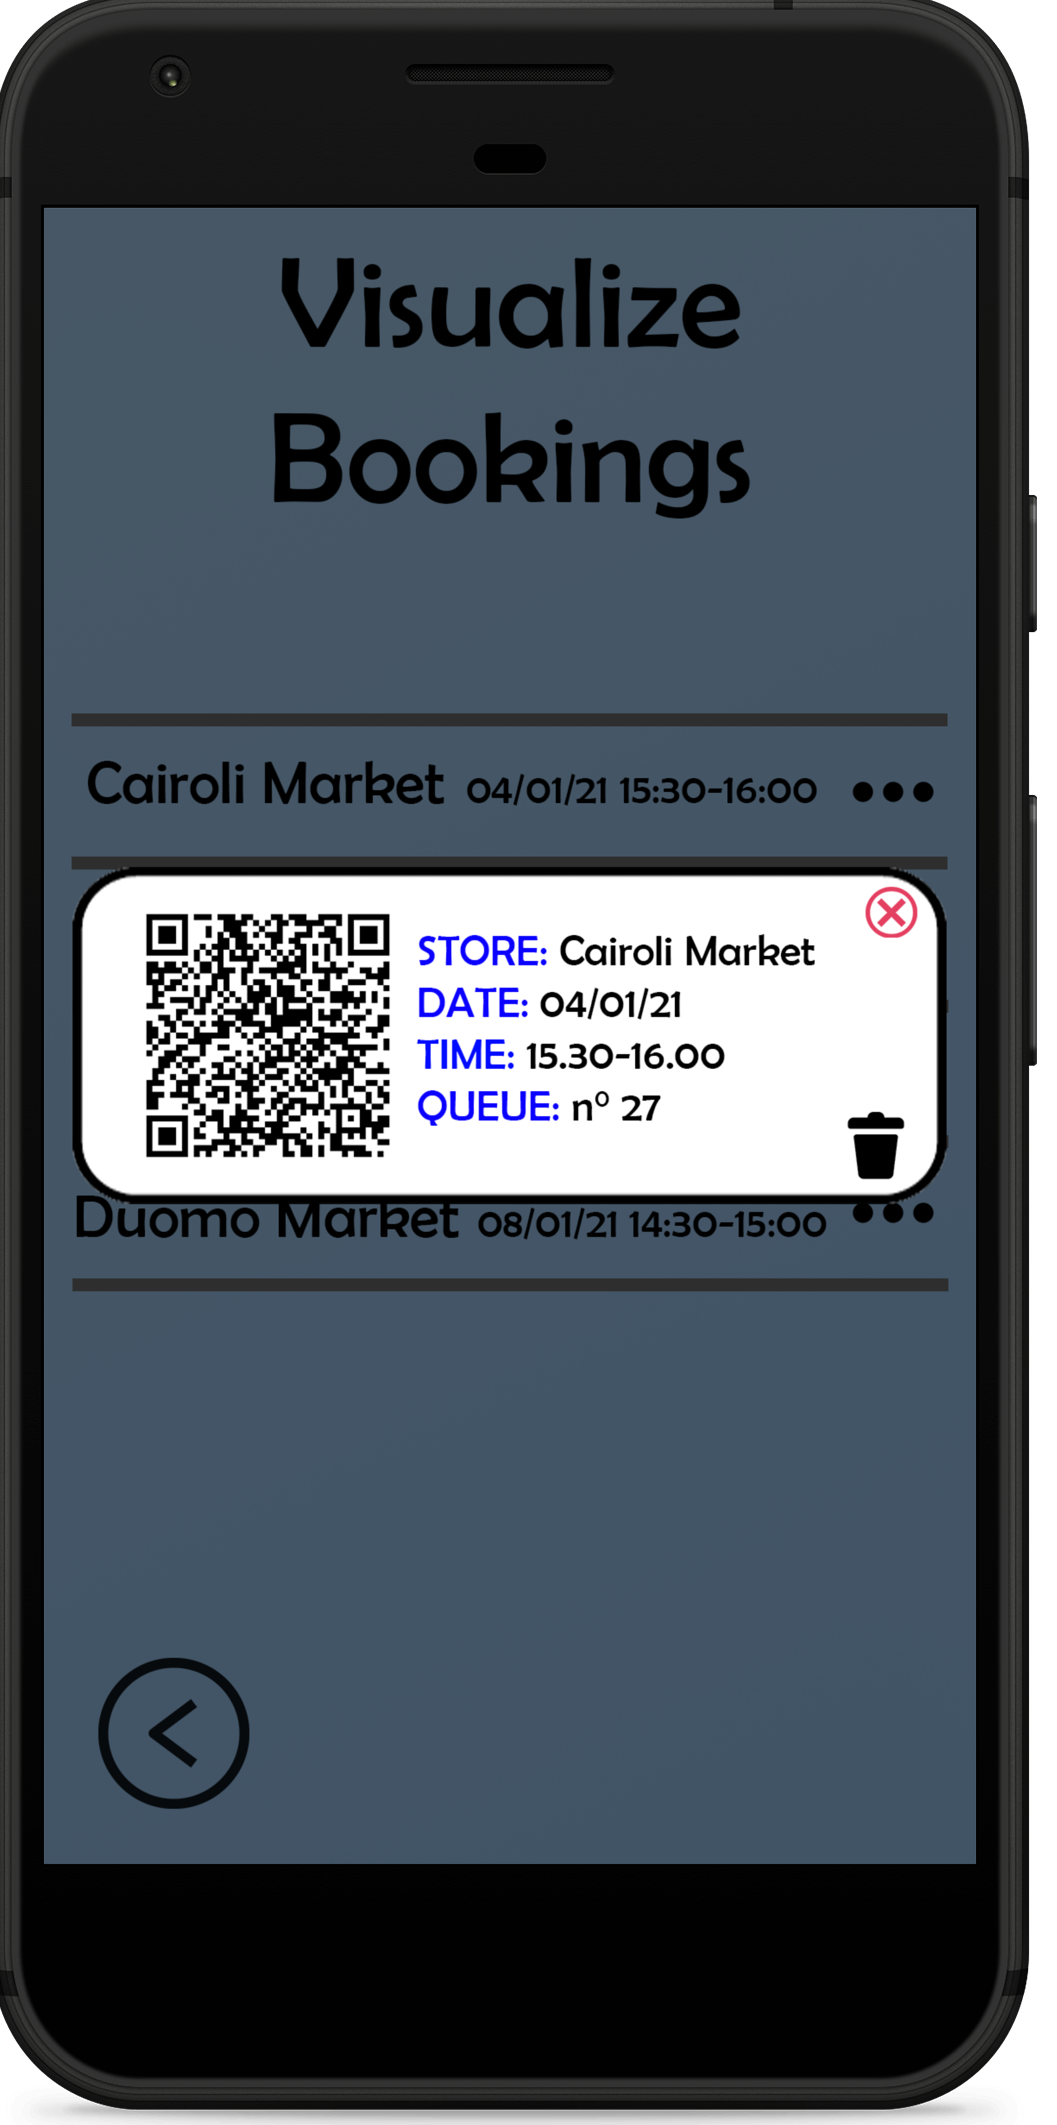
\includegraphics[width=\textwidth]{../Mockups/VBpopup.png}
				\caption{\emph{Visualize reservation detail}}
			\end{minipage}
		\end{figure}
		
		\newpage
		
		\subsubsection{Means of Transport}
		
		In this section is shown the mockup about means of transport. A customer can select his means of transport and that is very important beacuse, based on the choice made, all travel times are calculated accordingly. Moreover, means of transport used influence also the moment in which the notification, that warns the customer to leave his current position to reach the store in time, is sent.
		\bigskip
		\bigskip
		\begin{figure}[H]
			\begin{adjustwidth} {0cm}{}
				\centering
				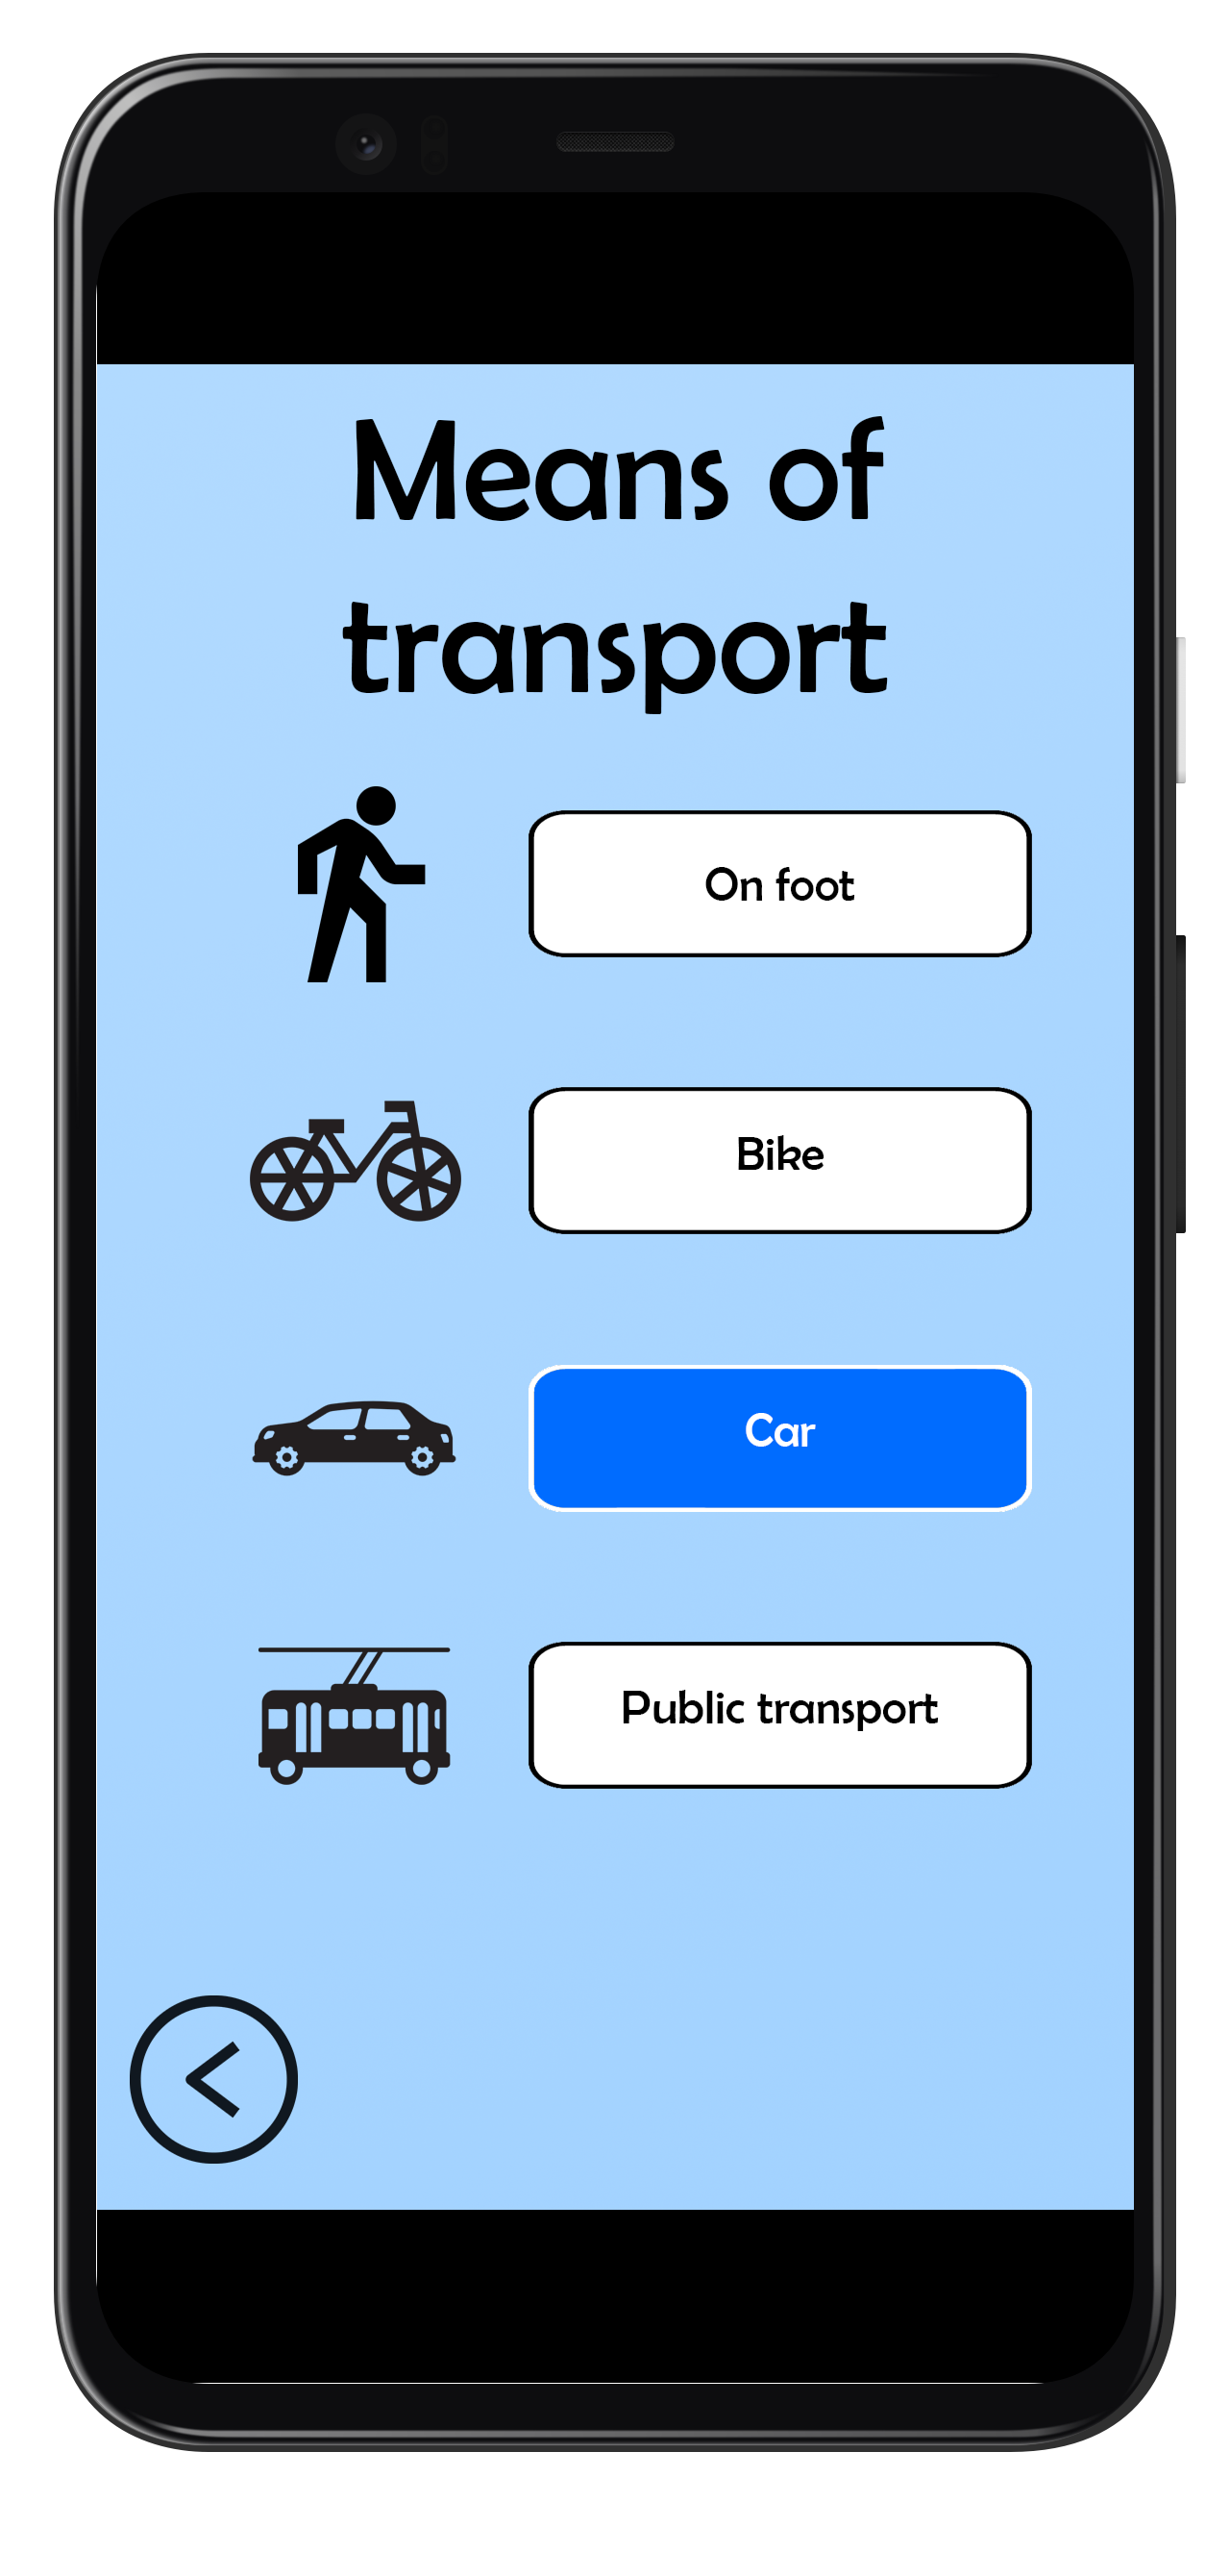
\includegraphics[scale=0.17]{../Mockups/MeansOfTransport.png}\\
			\end{adjustwidth}
			\caption{\emph{Means of transport}}
		\end{figure}
		
		\newpage
	
		\subsubsection{Manage Bookings}
		In this section are shown the mockups about the management of the customers' reservations. A store manager can:
		\begin{itemize}
			\item View the current entry queue
			\item Contact a customer via email
			\item Delete a customer reservation
			\item Reschedule a customer reservation
		\end{itemize}
		\bigskip
		\bigskip
		\begin{figure}[!h]
			\centering
			\begin{minipage}[!h]{0.4\textwidth}
				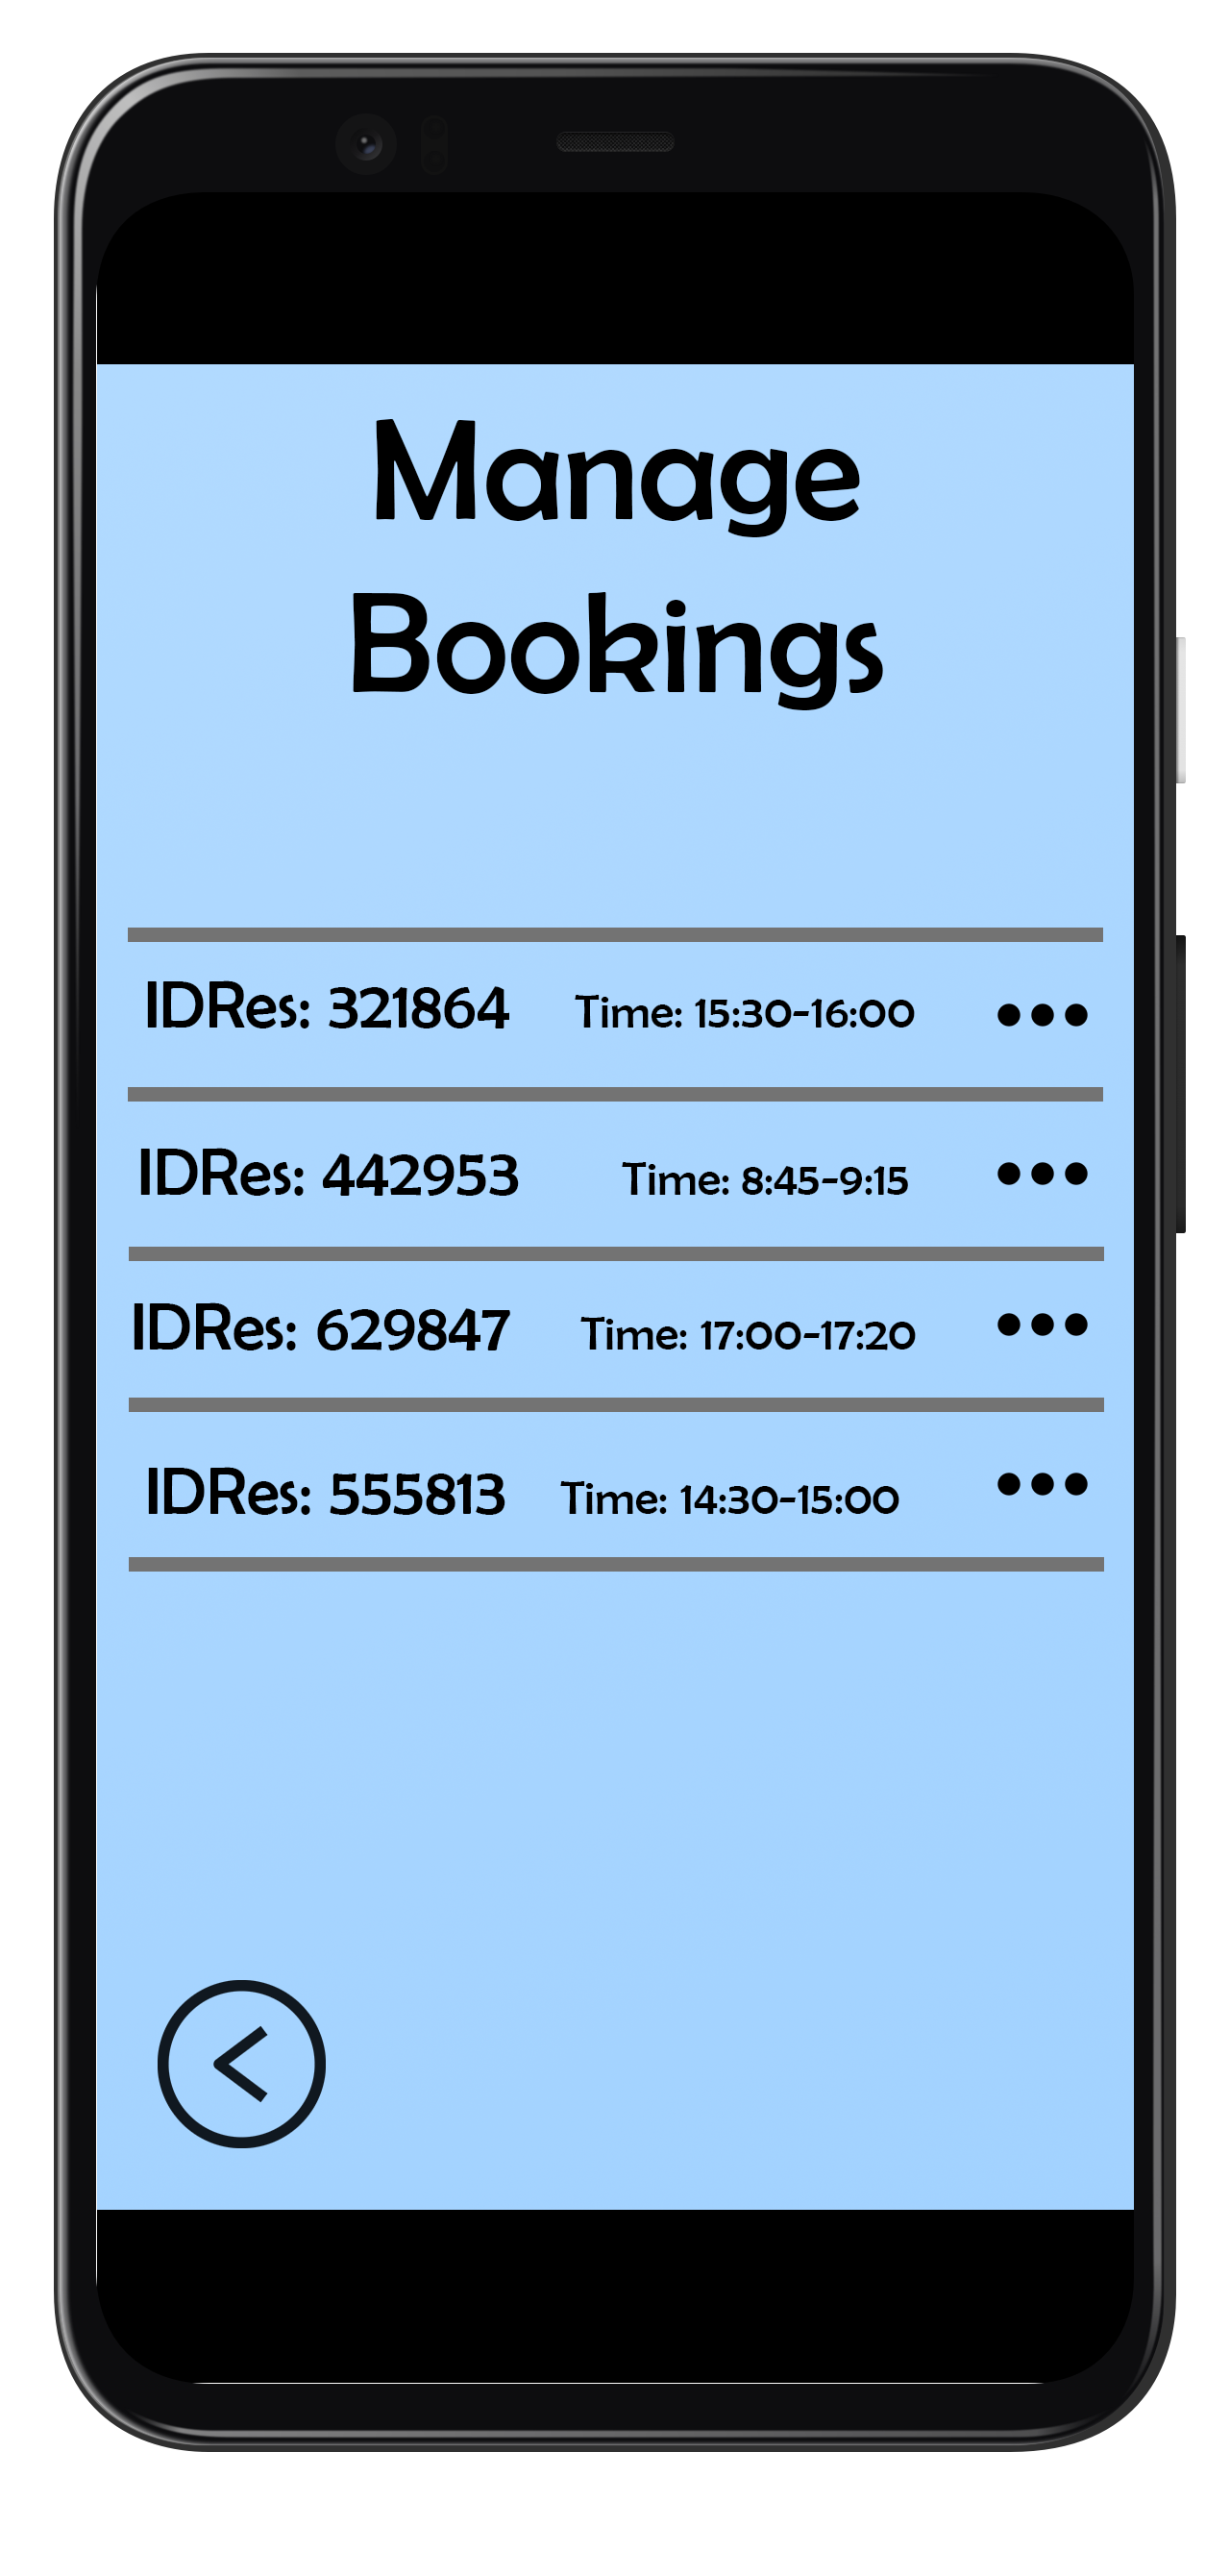
\includegraphics[width=\textwidth]{../Mockups/ManageBookings.png}
				\caption{\emph{Manage bookings}}
			\end{minipage}
			\hfill
			\begin{minipage}[!h]{0.4\textwidth}
				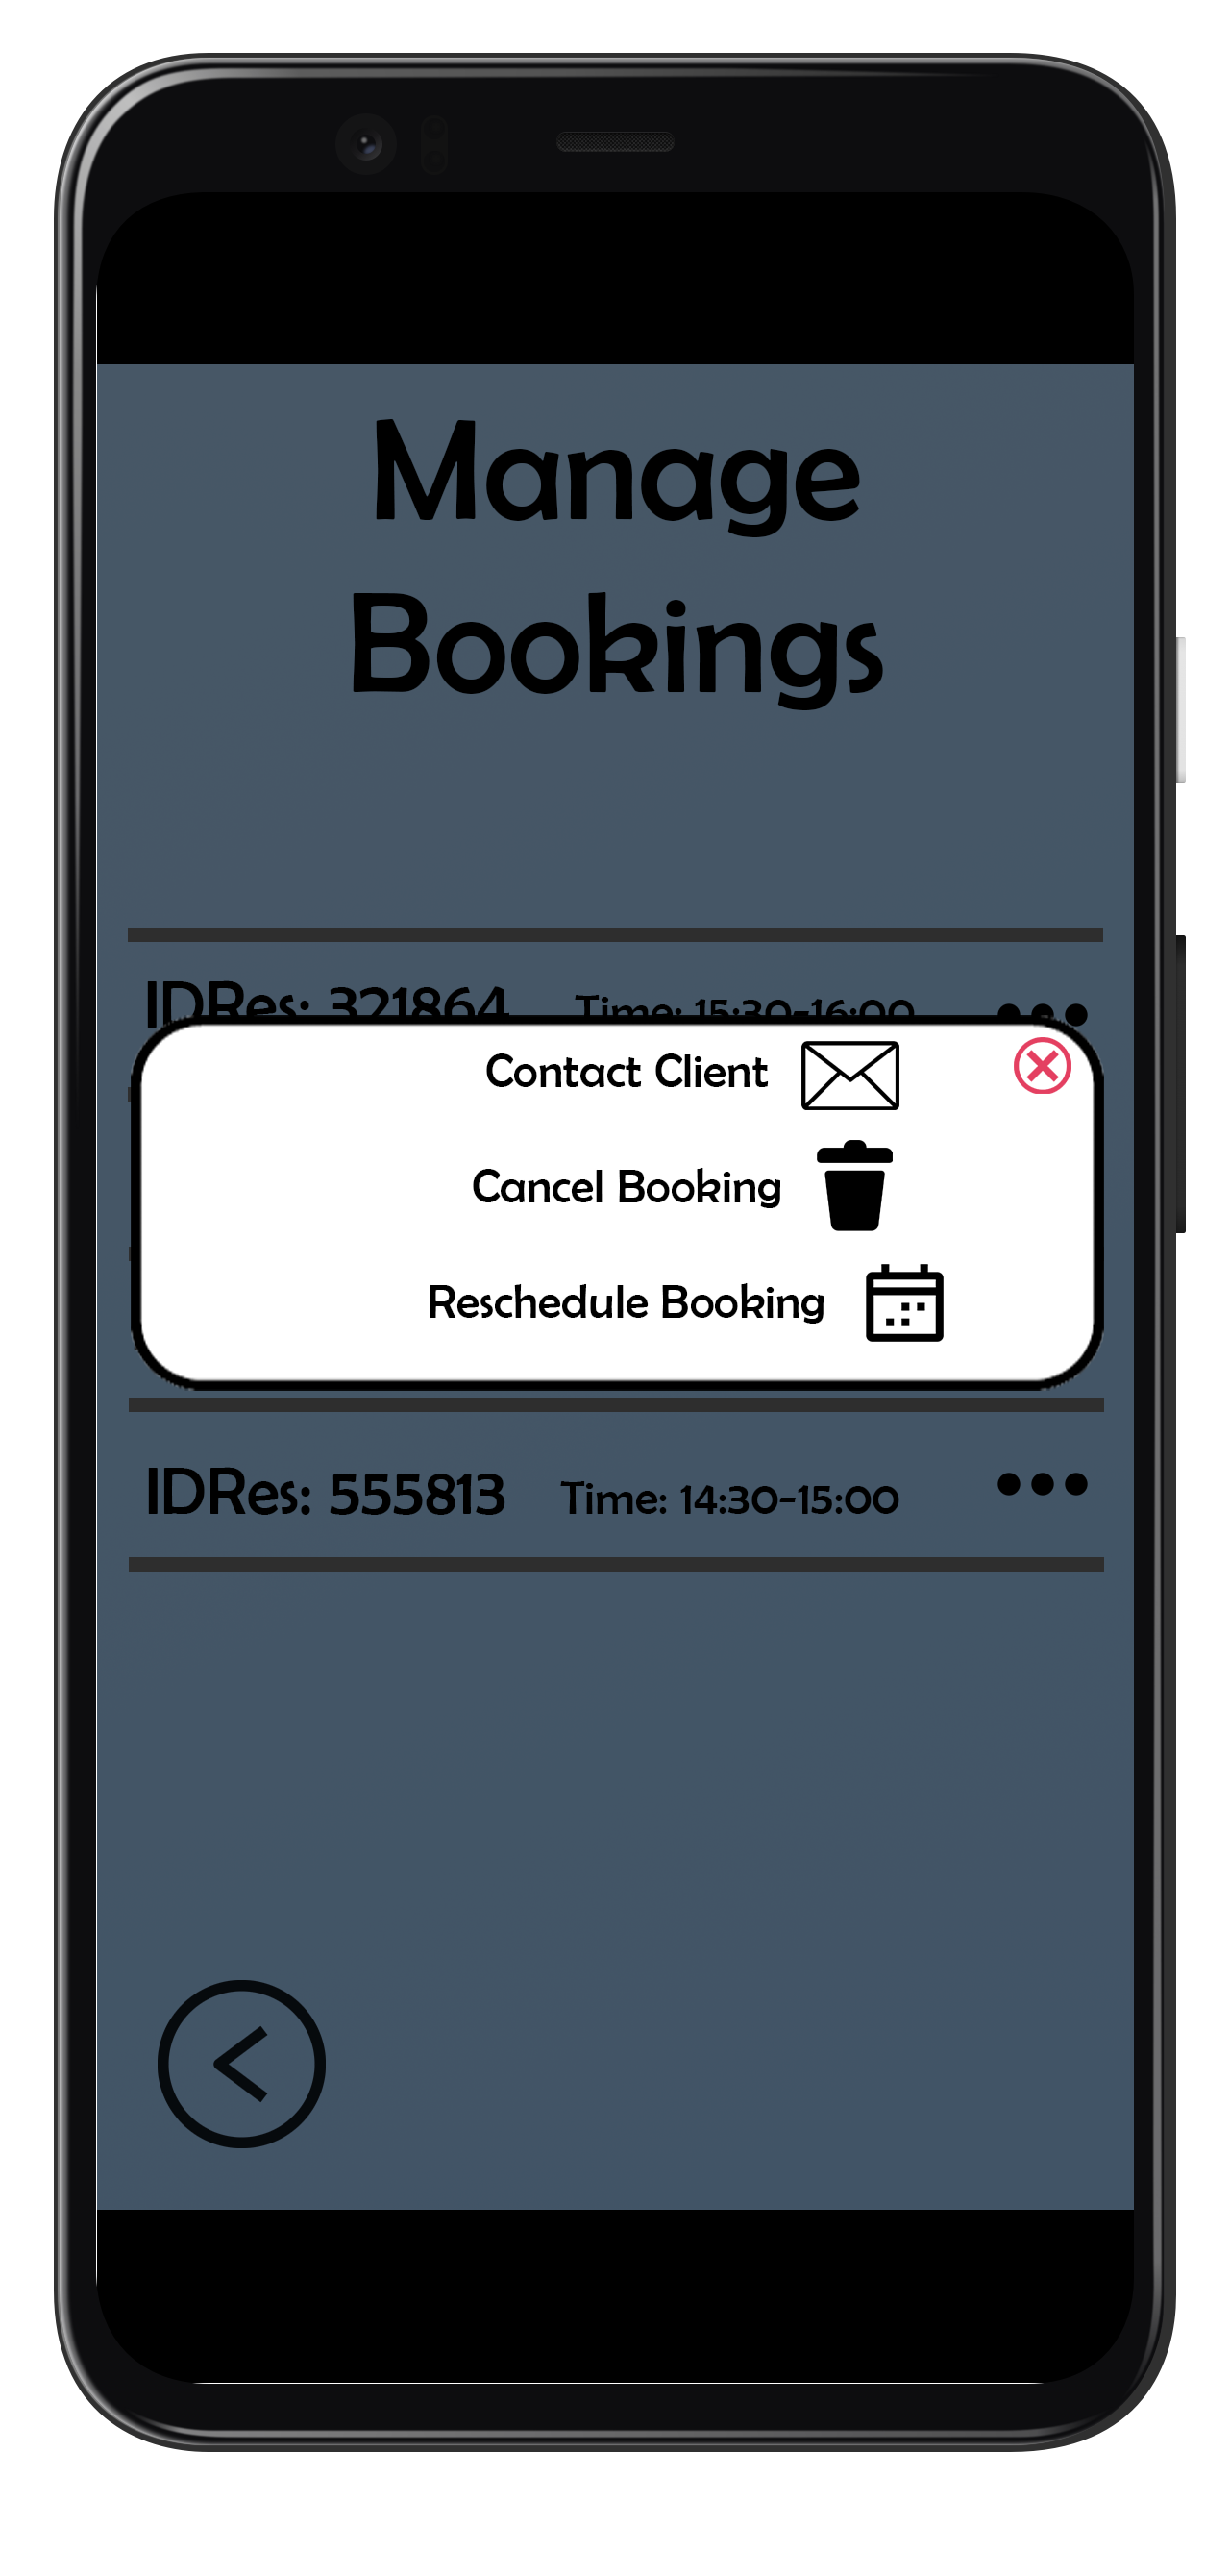
\includegraphics[width=\textwidth]{../Mockups/MBpopup.png}
				\caption{\emph{Manage bookings functionalities}}
			\end{minipage}
		\end{figure}
		\newpage
		\begin{figure}[!h]
			\centering
			\begin{minipage}[!h]{0.4\textwidth}
				\includegraphics[width=\textwidth]{../Mockups/MBpopup2.png}
				\caption{\emph{Contact customer via email}}
			\end{minipage}
			\hfill
			\begin{minipage}[!h]{0.4\textwidth}
				\includegraphics[width=\textwidth]{../Mockups/MBpopup3.png}
				\caption{\emph{Delete reservation}}
			\end{minipage}
		\end{figure}
	
		\newpage
		\newpage
		
		\subsubsection{Monitor store}
		
		In this section is shown the mockup about the store statistics. A store manager can view the statistics about flow of people inside the store, when he wants. Indeed statistics analyze the number of people that visit the store during an entire day and the time spent in average inside the store and each departments.
		\bigskip
		\bigskip
		\begin{figure}[!h]
			\begin{adjustwidth} {0cm}{}
				\centering
				\includegraphics[scale=0.17]{../Mockups/Statistics.png}\\
			\end{adjustwidth}
			\caption{\emph{Monitor statistics}}
		\end{figure}
		
		\newpage
		
		\subsubsection{Modify parameters}
		In this section is shown the mockup about the management of the store parameters. A store manager can decide to modify many personal parameters like Store \emph{ID} and password and many parameters that influence the customers' reservations. Indeed is possible to modify the opening and closure time of the store, the max simoultaneous booking per week by a customer and the capacity allowed for each deaprtments and for the entire store
		\bigskip
		\bigskip
		\begin{figure}[!h]
			\begin{adjustwidth} {0cm}{}
				\centering
				\includegraphics[scale=0.17]{../Mockups/ModifyParameters.png}\\
			\end{adjustwidth}
			\caption{\emph{Modify parameters}}
		\end{figure}
\section{Requirements Traceability}
In this section it is described how the requirements of the application are mapped to the components defined previously.

\begin{itemize}
\item {\bfseries R1}: The system must allow the customers to register \\
\textbf{AccessManager}

\item {\bfseries R2}: The system must allow store managers to register their store \\
\textbf{AccessManager}

\item {\bfseries R3}: The system must allow customers to log in \\
\textbf{AccessManager}

\item {\bfseries R4}: The system must allow store managers to log in \\ 
\textbf{AccessManager}

\item {\bfseries R5}: The system allows the customers to view their visits \\
\textbf{CustomerHandler}

\item {\bfseries R6}: The system allows the customers to cancel their visits \\
\textbf{CustomerHandler}

\item {\bfseries R7}: The system allows the customers to modify their visits \\
\textbf{CustomerHandler}

\item {\bfseries R8}: The system allows the customers to select their favourite means of transportation \\
\textbf{MobileApp}

\item {\bfseries R9}: The system allows customers to select the departments in which they are interested in doing shopping \\
\textbf{ReservationHandler}

\item {\bfseries R10}: The system must let in customers only if it's their turn \\
\textbf{StoreComponent}

\item {\bfseries R11}: The system must consider the estimate shopping time inserted by customers \\
\textbf{ReservationHandler}

\item {\bfseries R12}: The system must show the customers of the time periods in which they can enter the store, according to store's booking policies and the estimate of customers' shopping time \\
\textbf{DataManager}

\item {\bfseries R13}: The system have to make a reasonable estimate of when a user with a spot on the queue is able to enter the store \\
\textbf{StatisticComponent}

\item {\bfseries R14}: The system can send notification to the clients \\
\textbf{NotificationManager}

\item {\bfseries R15}: The system is able to ask for the position of the customers \\
\textbf{MapManager}

\item {\bfseries R16}: The system permits to store manager to modify some critical parameters of the store related to customers' affluence management \\
\textbf{StoreManagerHandler}

\item {\bfseries R17}: The system allows the manager to establish the maximum simultaneously allowed booked clients in a specific department \\
\textbf{StoreManagerHandler}

\item {\bfseries R18}: The store manager can cancel the reservation of each client \\
\textbf{StoreManagerHandler}

\item {\bfseries R19}: The store manager can modify the reservation of each client \\
\textbf{StoreManagerHandler}

\item {\bfseries R20}: The store manager can view the reservation of each client \\
\textbf{StoreManagerHandler}

\item {\bfseries R21}: The store manager can handle the working days and hours of the store, for each day of the week \\
\textbf{StoreManagerHandler}

\item {\bfseries R22}: The system knows the situation in real time of each store \\
\textbf{DataManager}

\item {\bfseries R23}: The system takes trace of each customer entry and exit from the store \\
\textbf{DataManager}

\item {\bfseries R24}: The system contains a list of bookable stores \\
\textbf{DataManager}

\item {\bfseries R25}: The system is able to print a paper ticket \\
\textbf{TotemApp}

\item {\bfseries R26}: The system can reasonably estimate the time needed from a customer to complete his shopping \\
\textbf{StatisticComponent}

\item {\bfseries R27}: The system saves clients' tickets \\
\textbf{DataManager}

\item {\bfseries R28}: The system is able to smartly call clients with a ticket to enter the building depending on reservations and people inside the building \\
\textbf{NumberCallingApp}

\item {\bfseries R29}: The system is able to scan and analyse a \emph{QR Code} \\
\textbf{ScannerApp}

\item{\bfseries R30}: The system is able to send emails \\
\textbf{MailComponent}

\item {\bfseries R31}: The system knows how the maximum number of bookings allowed weekly per customer \\
\textbf{DataManager}

\item{\bfseries R32}: The system can automatically rearrange reservations, if necessary \\
\textbf{DataManager}

\end{itemize}

\section{Implementation, Integration and Test Plan}
	\subsection{Overview}
	In this section we are going to show a clear plan on how implementation, integration and test plan should be done in order to optimize the work flow.
	
	After considered the various options available to define a \emph{Implementation Plan}, it's been decided to use the {\bfseries bottom-up approach}. So, each subcomponent will be developed, following an order different from to component to another, depending on the dependencies needed. Moreover, our system has been created with the intention of preserving modularity, in order to have loose coupling between components, thus simplifying future changes and maintenance. In the described plan, the component that can be simultaneously developed are grouped, to give an idea how the work can be managed in order to save time in the integration process.
	The first two components that must be implemented and integrated are {\bfseries StoreComponent} and {\bfseries CLupServer}.
	

		\subsection{StoreComponent}
		Before defining the Implementation Plan of the {\bfseries Store Component}, a \emph{Use Relation Hierarchy Diagram} have been traced, to understand the dependencies between the various components, so that an order of implementation can be defined.
		
		\begin{figure}[!h]
			\begin{adjustwidth} {-2cm}{}
				\centering
				\includegraphics[scale=0.4]{Hierchical Diagrams/StoreHierarchy.pdf}\\
			\end{adjustwidth}
			\caption{\emph{Use Relation Hierarchy Diagram of StoreComponent}}
		\end{figure}
				
		\begin{itemize}
		\item the components that have no other dependencies to others are {\bfseries DataManager}, {\bfseries MailComponent}, {\bfseries NotificationManager}. So, they are the first components that will be implemented. In particular,  {\bfseries DataManager} will be implemented after the installation of 			the \emph{DBMS}, to avoid the use of Stubs since the DBMS is already implemented and deployed, without need to test it. Instead, for {\bfseries NotificationManager} and {\bfseries MailComponent} there is the necessity to use some \emph{Drivers} waiting for the implementation of the components that uses them.  
		\item then, it's easy to implement the {\bfseries StatisticComponent}, integrating it with the already developed {\bfseries DataManager}, also using here some Drivers.
		\item at this point, the most critic part of the integration plan is about {\bfseries ParameterManager}, {\bfseries ReservationComponent} and {\bfseries CallingNumberComponent}, since are related in couple. For this reason, we can use some \emph{Drivers} and \emph{Stubs} for the other components not already implemented, but in the simultaneous development of the three, it's suggested to implement and integrate them using the "Thread" technique, so that the dependencies between them can be integrated going on with the work. Done the three component, it's possible to integrate them with the one they use, as reported in the graph ({\bfseries NotificationManager}, {\bfseries MailManager}, {\bfseries DataManager}). For {\bfseries CallingNumberComponent}, it's necessary to use some \emph{Stubs} to simulate the {\bfseries NumberCallingApp}, and some \emph{Drivers} for the {\bfseries ReservationComponent}.
		\item after that these have been completed, it's possible to implement {\bfseries FlowComponent}, {\bfseries RearrangeComponent} and {\bfseries StoreManagerHanlder}, without the need of using \emph{Stubs} or \emph{Driver} since their dependencies are implemented, but for {\bfseries ScannerApp}, for which a \emph{Driver} is needed in order to complete the testing of {\bfseries FlowComponent}.
		 \end{itemize}     
		 
		\subsection{CLupServer}
		
		\begin{figure}[!h]
			\begin{adjustwidth} {0cm}{}
				\centering
				\includegraphics[scale=0.5]{Hierchical Diagrams/ServerHierarchy.pdf}\\
			\end{adjustwidth}
			\caption{\emph{Use Relation Hierarchy Diagram of CLupServer}}
		\end{figure}	
		
		Also for {\bfseries CLupServer} a \emph{Use Relation Hierarchy Diagram} have been done, in order to identify the order with the single components can be implemented. 
		\begin{itemize}
		\item the first components that can be implemented are {\bfseries MailComponent} and {\bfseries DataManager}; as for the {\bfseries StoreComponent}, the {\bfseries DataManager} should be implemented and integrated after the associated \emph{DBMS} has been installed.
		\item then, it's possible to implement the {\bfseries AccessManager} and the {\bfseries ReservationHandler}, which can be integrated with the {\bfseries DataManager}. Some \emph{Drivers} simulating {\bfseries CustomerHandler} and {\bfseries MobileApp} are required to complete the test phase, and a \emph{Driver} is needed to simulate the {\bfseries StoreComponent} in testing the {\bfseries ReservationHandler}
		\item finally, the {\bfseries CustomerHandler} can be implemented, integrated with the {\bfseries ReservationHandler} and tested. In this last phase, is needed a \emph{Driver} to simulate the {\bfseries MobileApp}
		\end{itemize}
		
		After the previously described components have been developed, integrated and unit tested, it's possible to develop all the clients using them, and integrate the system in his completeness.
		

		

	
	\subsection{System Testing}
	Once the system is completely integrated, we can proceed testing it, to verify that functional and non-functional requirements are satisfied.
	In order to consider all the possible issues that our system could have, we have to test it in different ways:
	\begin{itemize}
		\item \textbf{Functional Testing}: ascertains that the system meet the functional requirements described in the RASD. Some tests that can be conducted are creating a reservation and check if it's created correctly, checking if correct suggestions are generated, trying the working of the management of QR Codes and of number calling. Moreover, also the correctness of calculation of statistics (and so of shopping time estimation) must be tested.
		\item \textbf{Performance Testing}: highlights problems related to the performance and bottlenecks; this test aims to check that the time constraint introduced in the RASD are respected, such as \emph{QR Codes} processing time, the time needed to call a new reservations and the one necessary to process a new one, general system responsiveness and departure notification generated in time
		\item \textbf{Load Testing}: highlights problems memory-related such as memory leaks and buffer overflows (e.g. verify if the system works even with a large number of customer and store manager operating at the same time, respecting the constraints of 200 simultaneous users per store registered in the system, as described in the RASD)
		\item \textbf{Stress Testing}: ascertains that the application recovers in the right way after failure (e.g. see what happens after an unexpected internet disconnection during an operation, and how the system responds to recover the data and operativity)
	\end{itemize}
			
	

\section{Effort Spent}
	
\bigskip
\bigskip

\begin{center}
	
	\renewcommand{\arraystretch}{1.2}
	
	\begin{tabular}[H]{|m{14em}|>{\centering\arraybackslash}m{12em}|}
		\rowcolor{gray!20}
		\hline
		\xrowht{5pt}
		\centering Task & Daniele Mammone's Hours \\
		\hline
		Introduction & 0 \\
		\hline
		Architectural Design & 0 \\
		\hline
		User Interface Design & 0 \\
		\hline
		Requirements Traceability & 0 \\
		\hline
		Implementation, Integration and Test Plan & 0 \\
		\hline
		Total Hours & 0\\
		\hline
	\end{tabular}
	
\end{center}

\bigskip
\bigskip

\begin{center}
	
	\renewcommand{\arraystretch}{1.2}
	
	\begin{tabular}[H]{|m{14em}|>{\centering\arraybackslash}m{12em}|}
	\rowcolor{gray!20}
	\hline
	\xrowht{5pt}
	\centering Task & Gianmarco Naro's Hours \\
	\hline
	Introduction & 0 \\
	\hline
	Architectural Design & 0 \\
	\hline
	User Interface Design & 0 \\
	\hline
	Requirements Traceability & 0 \\
	\hline
	Implementation, Integration and Test Plan & 0 \\
	\hline
	Total Hours & 0\\
	\hline
	\end{tabular}
\end{center}

\bigskip

\begin{center}
	
	\renewcommand{\arraystretch}{1.2}
	
	\begin{tabular}[H]{|m{14em}|>{\centering\arraybackslash}m{12em}|}
	\rowcolor{gray!20}
	\hline
	\xrowht{5pt}
	\centering Task & Massimo Parisi's Hours \\
	\hline
	Introduction & 0 \\
	\hline
	Architectural Design & 0 \\
	\hline
	User Interface Design & 0 \\
	\hline
	Requirements Traceability & 0 \\
	\hline
	Implementation, Integration and Test Plan & 0 \\
	\hline
	Total Hours & 0\\
	\hline
	\end{tabular}
\end{center}

\section{References}

\end{document}